% Options for packages loaded elsewhere
\PassOptionsToPackage{unicode}{hyperref}
\PassOptionsToPackage{hyphens}{url}
\PassOptionsToPackage{dvipsnames,svgnames,x11names}{xcolor}
%
\documentclass[
  letterpaper,
  pandoc,
  ja=standard,
  jafont = hiragino-pron]{ltjsbook}

\usepackage{amsmath,amssymb}
\usepackage{iftex}
\ifPDFTeX
  \usepackage[T1]{fontenc}
  \usepackage[utf8]{inputenc}
  \usepackage{textcomp} % provide euro and other symbols
\else % if luatex or xetex
  \usepackage{unicode-math}
  \defaultfontfeatures{Scale=MatchLowercase}
  \defaultfontfeatures[\rmfamily]{Ligatures=TeX,Scale=1}
\fi
\usepackage{lmodern}
\ifPDFTeX\else  
    % xetex/luatex font selection
\fi
% Use upquote if available, for straight quotes in verbatim environments
\IfFileExists{upquote.sty}{\usepackage{upquote}}{}
\IfFileExists{microtype.sty}{% use microtype if available
  \usepackage[]{microtype}
  \UseMicrotypeSet[protrusion]{basicmath} % disable protrusion for tt fonts
}{}
\makeatletter
\@ifundefined{KOMAClassName}{% if non-KOMA class
  \IfFileExists{parskip.sty}{%
    \usepackage{parskip}
  }{% else
    \setlength{\parindent}{0pt}
    \setlength{\parskip}{6pt plus 2pt minus 1pt}}
}{% if KOMA class
  \KOMAoptions{parskip=half}}
\makeatother
\usepackage{xcolor}
\setlength{\emergencystretch}{3em} % prevent overfull lines
\setcounter{secnumdepth}{5}
% Make \paragraph and \subparagraph free-standing
\makeatletter
\ifx\paragraph\undefined\else
  \let\oldparagraph\paragraph
  \renewcommand{\paragraph}{
    \@ifstar
      \xxxParagraphStar
      \xxxParagraphNoStar
  }
  \newcommand{\xxxParagraphStar}[1]{\oldparagraph*{#1}\mbox{}}
  \newcommand{\xxxParagraphNoStar}[1]{\oldparagraph{#1}\mbox{}}
\fi
\ifx\subparagraph\undefined\else
  \let\oldsubparagraph\subparagraph
  \renewcommand{\subparagraph}{
    \@ifstar
      \xxxSubParagraphStar
      \xxxSubParagraphNoStar
  }
  \newcommand{\xxxSubParagraphStar}[1]{\oldsubparagraph*{#1}\mbox{}}
  \newcommand{\xxxSubParagraphNoStar}[1]{\oldsubparagraph{#1}\mbox{}}
\fi
\makeatother

\usepackage{color}
\usepackage{fancyvrb}
\newcommand{\VerbBar}{|}
\newcommand{\VERB}{\Verb[commandchars=\\\{\}]}
\DefineVerbatimEnvironment{Highlighting}{Verbatim}{commandchars=\\\{\}}
% Add ',fontsize=\small' for more characters per line
\usepackage{framed}
\definecolor{shadecolor}{RGB}{241,243,245}
\newenvironment{Shaded}{\begin{snugshade}}{\end{snugshade}}
\newcommand{\AlertTok}[1]{\textcolor[rgb]{0.68,0.00,0.00}{#1}}
\newcommand{\AnnotationTok}[1]{\textcolor[rgb]{0.37,0.37,0.37}{#1}}
\newcommand{\AttributeTok}[1]{\textcolor[rgb]{0.40,0.45,0.13}{#1}}
\newcommand{\BaseNTok}[1]{\textcolor[rgb]{0.68,0.00,0.00}{#1}}
\newcommand{\BuiltInTok}[1]{\textcolor[rgb]{0.00,0.23,0.31}{#1}}
\newcommand{\CharTok}[1]{\textcolor[rgb]{0.13,0.47,0.30}{#1}}
\newcommand{\CommentTok}[1]{\textcolor[rgb]{0.37,0.37,0.37}{#1}}
\newcommand{\CommentVarTok}[1]{\textcolor[rgb]{0.37,0.37,0.37}{\textit{#1}}}
\newcommand{\ConstantTok}[1]{\textcolor[rgb]{0.56,0.35,0.01}{#1}}
\newcommand{\ControlFlowTok}[1]{\textcolor[rgb]{0.00,0.23,0.31}{\textbf{#1}}}
\newcommand{\DataTypeTok}[1]{\textcolor[rgb]{0.68,0.00,0.00}{#1}}
\newcommand{\DecValTok}[1]{\textcolor[rgb]{0.68,0.00,0.00}{#1}}
\newcommand{\DocumentationTok}[1]{\textcolor[rgb]{0.37,0.37,0.37}{\textit{#1}}}
\newcommand{\ErrorTok}[1]{\textcolor[rgb]{0.68,0.00,0.00}{#1}}
\newcommand{\ExtensionTok}[1]{\textcolor[rgb]{0.00,0.23,0.31}{#1}}
\newcommand{\FloatTok}[1]{\textcolor[rgb]{0.68,0.00,0.00}{#1}}
\newcommand{\FunctionTok}[1]{\textcolor[rgb]{0.28,0.35,0.67}{#1}}
\newcommand{\ImportTok}[1]{\textcolor[rgb]{0.00,0.46,0.62}{#1}}
\newcommand{\InformationTok}[1]{\textcolor[rgb]{0.37,0.37,0.37}{#1}}
\newcommand{\KeywordTok}[1]{\textcolor[rgb]{0.00,0.23,0.31}{\textbf{#1}}}
\newcommand{\NormalTok}[1]{\textcolor[rgb]{0.00,0.23,0.31}{#1}}
\newcommand{\OperatorTok}[1]{\textcolor[rgb]{0.37,0.37,0.37}{#1}}
\newcommand{\OtherTok}[1]{\textcolor[rgb]{0.00,0.23,0.31}{#1}}
\newcommand{\PreprocessorTok}[1]{\textcolor[rgb]{0.68,0.00,0.00}{#1}}
\newcommand{\RegionMarkerTok}[1]{\textcolor[rgb]{0.00,0.23,0.31}{#1}}
\newcommand{\SpecialCharTok}[1]{\textcolor[rgb]{0.37,0.37,0.37}{#1}}
\newcommand{\SpecialStringTok}[1]{\textcolor[rgb]{0.13,0.47,0.30}{#1}}
\newcommand{\StringTok}[1]{\textcolor[rgb]{0.13,0.47,0.30}{#1}}
\newcommand{\VariableTok}[1]{\textcolor[rgb]{0.07,0.07,0.07}{#1}}
\newcommand{\VerbatimStringTok}[1]{\textcolor[rgb]{0.13,0.47,0.30}{#1}}
\newcommand{\WarningTok}[1]{\textcolor[rgb]{0.37,0.37,0.37}{\textit{#1}}}

\providecommand{\tightlist}{%
  \setlength{\itemsep}{0pt}\setlength{\parskip}{0pt}}\usepackage{longtable,booktabs,array}
\usepackage{calc} % for calculating minipage widths
% Correct order of tables after \paragraph or \subparagraph
\usepackage{etoolbox}
\makeatletter
\patchcmd\longtable{\par}{\if@noskipsec\mbox{}\fi\par}{}{}
\makeatother
% Allow footnotes in longtable head/foot
\IfFileExists{footnotehyper.sty}{\usepackage{footnotehyper}}{\usepackage{footnote}}
\makesavenoteenv{longtable}
\usepackage{graphicx}
\makeatletter
\newsavebox\pandoc@box
\newcommand*\pandocbounded[1]{% scales image to fit in text height/width
  \sbox\pandoc@box{#1}%
  \Gscale@div\@tempa{\textheight}{\dimexpr\ht\pandoc@box+\dp\pandoc@box\relax}%
  \Gscale@div\@tempb{\linewidth}{\wd\pandoc@box}%
  \ifdim\@tempb\p@<\@tempa\p@\let\@tempa\@tempb\fi% select the smaller of both
  \ifdim\@tempa\p@<\p@\scalebox{\@tempa}{\usebox\pandoc@box}%
  \else\usebox{\pandoc@box}%
  \fi%
}
% Set default figure placement to htbp
\def\fps@figure{htbp}
\makeatother

\makeatletter
\@ifpackageloaded{tcolorbox}{}{\usepackage[skins,breakable]{tcolorbox}}
\@ifpackageloaded{fontawesome5}{}{\usepackage{fontawesome5}}
\definecolor{quarto-callout-color}{HTML}{909090}
\definecolor{quarto-callout-note-color}{HTML}{0758E5}
\definecolor{quarto-callout-important-color}{HTML}{CC1914}
\definecolor{quarto-callout-warning-color}{HTML}{EB9113}
\definecolor{quarto-callout-tip-color}{HTML}{00A047}
\definecolor{quarto-callout-caution-color}{HTML}{FC5300}
\definecolor{quarto-callout-color-frame}{HTML}{acacac}
\definecolor{quarto-callout-note-color-frame}{HTML}{4582ec}
\definecolor{quarto-callout-important-color-frame}{HTML}{d9534f}
\definecolor{quarto-callout-warning-color-frame}{HTML}{f0ad4e}
\definecolor{quarto-callout-tip-color-frame}{HTML}{02b875}
\definecolor{quarto-callout-caution-color-frame}{HTML}{fd7e14}
\makeatother
\makeatletter
\@ifpackageloaded{bookmark}{}{\usepackage{bookmark}}
\makeatother
\makeatletter
\@ifpackageloaded{caption}{}{\usepackage{caption}}
\AtBeginDocument{%
\ifdefined\contentsname
  \renewcommand*\contentsname{Table of contents}
\else
  \newcommand\contentsname{Table of contents}
\fi
\ifdefined\listfigurename
  \renewcommand*\listfigurename{List of Figures}
\else
  \newcommand\listfigurename{List of Figures}
\fi
\ifdefined\listtablename
  \renewcommand*\listtablename{List of Tables}
\else
  \newcommand\listtablename{List of Tables}
\fi
\ifdefined\figurename
  \renewcommand*\figurename{Figure}
\else
  \newcommand\figurename{Figure}
\fi
\ifdefined\tablename
  \renewcommand*\tablename{Table}
\else
  \newcommand\tablename{Table}
\fi
}
\@ifpackageloaded{float}{}{\usepackage{float}}
\floatstyle{ruled}
\@ifundefined{c@chapter}{\newfloat{codelisting}{h}{lop}}{\newfloat{codelisting}{h}{lop}[chapter]}
\floatname{codelisting}{Listing}
\newcommand*\listoflistings{\listof{codelisting}{List of Listings}}
\makeatother
\makeatletter
\makeatother
\makeatletter
\@ifpackageloaded{caption}{}{\usepackage{caption}}
\@ifpackageloaded{subcaption}{}{\usepackage{subcaption}}
\makeatother
\makeatletter
\@ifpackageloaded{tcolorbox}{}{\usepackage[skins,breakable]{tcolorbox}}
\makeatother
\makeatletter
\@ifundefined{shadecolor}{\definecolor{shadecolor}{rgb}{.97, .97, .97}}{}
\makeatother
\makeatletter
\@ifundefined{codebgcolor}{\definecolor{codebgcolor}{HTML}{F6F6F6}}{}
\makeatother
\makeatletter
\ifdefined\Shaded\renewenvironment{Shaded}{\begin{tcolorbox}[sharp corners, frame hidden, enhanced, colback={codebgcolor}, boxrule=0pt, breakable]}{\end{tcolorbox}}\fi
\makeatother

\usepackage{bookmark}

\IfFileExists{xurl.sty}{\usepackage{xurl}}{} % add URL line breaks if available
\urlstyle{same} % disable monospaced font for URLs
\hypersetup{
  pdftitle={畠田 証券投資論},
  pdfauthor={松浦総一},
  colorlinks=true,
  linkcolor={blue},
  filecolor={Maroon},
  citecolor={Blue},
  urlcolor={Blue},
  pdfcreator={LaTeX via pandoc}}


\title{畠田 証券投資論}
\author{松浦総一}
\date{2023-07-24}

\begin{document}
\maketitle

\renewcommand*\contentsname{Table of contents}
{
\hypersetup{linkcolor=}
\setcounter{tocdepth}{1}
\tableofcontents
}

\bookmarksetup{startatroot}

\chapter{はじめに}\label{ux306fux3058ux3081ux306b}

この資料は,神戸大学経営学研究科の畠田先生が立命館大学で開講した「証券投資論」という科目の資料をもとに,ファイナンスの基礎を学習するためのノートとして松浦が再編集したものです。
この資料の元ネタは,{証券アナリスト協会が証券アナリスト試験の教材として推奨している教科書}

\begin{itemize}
\tightlist
\item
  小林孝雄,芹田敏夫 (2009) 「\textbf{新・証券投資論 I
  理論編}」日本経済新聞社
\end{itemize}

です。
この教科書は,ファイナンスの基礎理論を体系的に学ぶことができる良書ですので,この資料とともに教科書も随時参照するようにしてください。
ファイナンスの基礎を理解するためには,確率論と統計学の基礎知識が必要です。そのための参考書として以下のものがオススメです。

\begin{enumerate}
\def\labelenumi{\arabic{enumi}.}
\tightlist
\item
  石井俊全 著 (2018) 「\textbf{1冊でマスター 大学の統計学}」 技術評論社
\item
  木村俊一,鈴川晶夫,古澄英男 (2003) 「\textbf{確率と統計 --
  基礎と応用}」 朝倉書店
\item
  森棟公夫・照井伸彦・中川満・西埜晴久・黒住英司 著「\textbf{統計学}」
  有斐閣
\item
  西山慶彦・新谷元嗣・川口大司・奥井亮 著 (2019) 「\textbf{計量経済学}」
  有斐閣
\item
  浅野皙・中村二朗 著 (2009)「\textbf{計量経済学} 第2版」有斐閣
\item
  山本拓 (2022)「\textbf{計量経済学} 第2版」 新世社
\end{enumerate}

1は統計学の基礎を学ぶ教科書・問題集となっていて,独学に最適な教科書です。
2と3は統計学の基礎をしっかり学びたい人向けの,数学的な厳密性を重視した教科書です。
4は計量経済学の基礎から応用まで幅広く,かつ厳密に学ぶための教科書です。
5と6は4と同様に計量経済学の基礎を学ぶ教科書ですが,5はパネルデータ分析に詳しく,6は時系列分析に詳しいです。

この教科書では触れられていない行動ファイナンスの知識については,

\begin{itemize}
\tightlist
\item
  Shefrin, H. (2002) ``\textbf{Beyond Greed and Fear}'', Oxford
  University Press, Chapter 1-4.
  (鈴木一功訳「行動ファイナンスと投資の心理学」東洋経済新報社,2005年)
\item
  Montier, J, (2002) ``\textbf{Behavioural Finance: Insights into
  irrational minds and markets}'', Wiley \& Sons, Chapter 1.
  (真壁昭夫,川西諭、栗田昌孝訳「行動ファイナンスの実践 --
  投資家心理が動かす金融市場を読む---」,ダイヤモンド社,2005年)
\end{itemize}

で補います。

\section{1.
授業のテーマと到達目標}\label{ux6388ux696dux306eux30c6ux30fcux30deux3068ux5230ux9054ux76eeux6a19}

ファイナンスは,大きく分けると,\textbf{金融市場}(証券市場)とコーポレートファイナンスの分野に大別されます。
金融市場は金融資産への投資問題に焦点を向けることで,リターンとリスクの関係,ポートフォリオ選択,資産の価格づけ,リスクマネジメントを明らかにしようとする分野です。
本講義では,先ず,それらの内容について詳細に解説を行うことで,伝統的な証券投資論の考え方を理解します。
そして,その上で,最近,積極的に議論されている行動ファイナンスの考え方についての解説を行います。

\bookmarksetup{startatroot}

\chapter{確率}\label{ux78baux7387}

東証株価指数(Tokyo Stock Price Index: TOPIX)の値動きから何を感じますか?
以下では、TOPIXの動きを通して確率について学びます。

まずは、Rの環境を整えましょう。
いくつかのパッケージを読み込み,グラフ作成時のスタイルを設定しておきます。

\begin{Shaded}
\begin{Highlighting}[]
\NormalTok{pacman}\SpecialCharTok{::}\FunctionTok{p\_load}\NormalTok{(tidyverse, ggthemes, patchwork)}
\end{Highlighting}
\end{Shaded}

次にTOPIXのデータを読み込みんで、TOPIXの動きを確認します。
ここで読み込んでいる\texttt{stock\_data.csv}には,2007年4月2日から2023年4月28日にわたる,TOPIX,トヨタ自動車,日産自動車,本田技術研究所の株価の終値が日次で記録されています。

\begin{Shaded}
\begin{Highlighting}[]
\NormalTok{df }\OtherTok{\textless{}{-}} \FunctionTok{read\_csv}\NormalTok{(}\StringTok{"data/stock\_data.csv"}\NormalTok{)}
\end{Highlighting}
\end{Shaded}

ここで,TOPIXとは,東京証券取引所一部上場株式銘柄を対象として東京証券取引所が1秒ごとに算出・公表している株式ポートフォリオ(東証一部の時価総額)を株価指数で表したものです。
他の株価指数として有名なものに日経株価平均があります。
TOPIXの値動きを確認してみましょう。

\begin{Shaded}
\begin{Highlighting}[]
\FunctionTok{ggplot}\NormalTok{(df) }\SpecialCharTok{+} \FunctionTok{aes}\NormalTok{(}\AttributeTok{x =}\NormalTok{ date, }\AttributeTok{y =}\NormalTok{ TOPIX) }\SpecialCharTok{+} \FunctionTok{geom\_line}\NormalTok{()}
\end{Highlighting}
\end{Shaded}

\pandocbounded{\includegraphics[keepaspectratio]{Hatakeda_Chap02_files/figure-pdf/unnamed-chunk-2-1.pdf}}

2008年のリーマンショックで暴落した株価も2014年からはじまったアベノミクスで株価は上昇し,2016年のマイナス金利,2020年の新型コロナウイルスの感染拡大による株価の下落など,TOPIXの値動きは経済の動向を反映していることが分かります。

\section{期待値と分散(標準偏差)の推定}\label{ux671fux5f85ux5024ux3068ux5206ux6563ux6a19ux6e96ux504fux5deeux306eux63a8ux5b9a}

ファイナンスの分野では,資産価値(たとえば株価)それ自体より,\textbf{資産価値の変化率}(これを\textbf{リターン}といいます)で議論することも多いです。
先のTOPIXのデータを使って,TOPIXのリターンを計算して作図してみましょう。
まずリターン(return)の定義を確認します。

\begin{tcolorbox}[enhanced jigsaw, colframe=quarto-callout-important-color-frame, breakable, rightrule=.15mm, coltitle=black, title=\textcolor{quarto-callout-important-color}{\faExclamation}\hspace{0.5em}{リターン}, colbacktitle=quarto-callout-important-color!10!white, leftrule=.75mm, colback=white, left=2mm, arc=.35mm, opacityback=0, titlerule=0mm, toptitle=1mm, bottomtitle=1mm, bottomrule=.15mm, toprule=.15mm, opacitybacktitle=0.6]

資産\(i\)の\(t\)期のリターン\(r_{i,t}\)は,

\[
\begin{aligned}
r_{i,t} &= \frac{D_{i,t} + (P_{i,t} - P_{i,t-1})}{P_{i,t-1}} \\
%&= \frac{D_{i,t}}{P_{i,t-1}} + \frac{P_{i,t} - P_{i,t-1}}{P_{i,t-1}}\\
&= \frac{D_{i,t} - P_{i,t}}{P_{i,t-1}} -1
\end{aligned}
\]

ここで

\begin{itemize}
\tightlist
\item
  \(D\)はインカム(配当,クーポン,地代など)
\item
  \(P\)は資産価値(株価,債券価格,地価など)
\item
  \(i\)は企業,\(t\)は期を表す。
\end{itemize}

\end{tcolorbox}

配当を受け取った場合,配当落ち日次リターンを計算することになります。上の式から配当\(D\)を引いて計算します。

\begin{tcolorbox}[enhanced jigsaw, colframe=quarto-callout-important-color-frame, breakable, rightrule=.15mm, coltitle=black, title=\textcolor{quarto-callout-important-color}{\faExclamation}\hspace{0.5em}{配当落ち日次リターン}, colbacktitle=quarto-callout-important-color!10!white, leftrule=.75mm, colback=white, left=2mm, arc=.35mm, opacityback=0, titlerule=0mm, toptitle=1mm, bottomtitle=1mm, bottomrule=.15mm, toprule=.15mm, opacitybacktitle=0.6]

株式\(i\)の\(t\)期における(配当落ち)日次リターン\(r_{i,t}\)は,

\[
\begin{aligned}
r_{i,t} = \frac{P_{i,t} - P_{i,t-1}}{P_{i,t-1}} = \frac{P_{i,t}}{P_{i,t-1}} - 1
\end{aligned}
\]

株式の日次リターンを上の式に従って計算する場合,インカムゲインは考慮されていないことに留意しましょう。

\end{tcolorbox}

同様に,TOPIXの(配当落ち)リターン\(r^{TOPIX}_{i,t}\)は

\[
\begin{aligned}
r^{TOPIX}_{i,t} = \frac{p_{i,t}}{p_{i,t-1}} - 1
\end{aligned}
\]

となります。具体的には、次のような表になります。

\begin{Shaded}
\begin{Highlighting}[]
\CommentTok{\# リターンの計算}
\NormalTok{df }\OtherTok{\textless{}{-}}\NormalTok{ df }\SpecialCharTok{\%\textgreater{}\%}
  \FunctionTok{mutate}\NormalTok{(}
      \AttributeTok{TOPIX\_return =}\NormalTok{ TOPIX }\SpecialCharTok{/} \FunctionTok{lag}\NormalTok{(TOPIX) }\SpecialCharTok{{-}} \DecValTok{1} \CommentTok{\# TOPIXのリターン}
\NormalTok{      )}
\CommentTok{\# 作表}
\NormalTok{df }\SpecialCharTok{\%\textgreater{}\%}
  \FunctionTok{select}\NormalTok{(date, TOPIX, TOPIX\_return) }\SpecialCharTok{\%\textgreater{}\%}
  \FunctionTok{head}\NormalTok{(}\DecValTok{10}\NormalTok{) }\SpecialCharTok{\%\textgreater{}\%}
\NormalTok{  knitr}\SpecialCharTok{::}\FunctionTok{kable}\NormalTok{(}\AttributeTok{digits =} \DecValTok{3}\NormalTok{, }\AttributeTok{booktabs =} \ConstantTok{TRUE}\NormalTok{)}
\end{Highlighting}
\end{Shaded}

\begin{longtable}[]{@{}lrr@{}}
\toprule\noalign{}
date & TOPIX & TOPIX\_return \\
\midrule\noalign{}
\endhead
\bottomrule\noalign{}
\endlastfoot
2007-04-02 & 1682.49 & NA \\
2007-04-03 & 1704.32 & 0.013 \\
2007-04-04 & 1730.52 & 0.015 \\
2007-04-05 & 1720.72 & -0.006 \\
2007-04-06 & 1717.08 & -0.002 \\
2007-04-09 & 1738.10 & 0.012 \\
2007-04-10 & 1735.69 & -0.001 \\
2007-04-11 & 1739.01 & 0.002 \\
2007-04-12 & 1726.18 & -0.007 \\
2007-04-13 & 1705.50 & -0.012 \\
\end{longtable}

この\texttt{TOPIX\_return}を折れ線グラフにすると以下のようになります。

\begin{Shaded}
\begin{Highlighting}[]
\FunctionTok{ggplot}\NormalTok{(df) }\SpecialCharTok{+} \FunctionTok{aes}\NormalTok{(}\AttributeTok{x =}\NormalTok{ date, }\AttributeTok{y =}\NormalTok{ TOPIX\_return) }\SpecialCharTok{+} \FunctionTok{geom\_line}\NormalTok{()}
\end{Highlighting}
\end{Shaded}

\pandocbounded{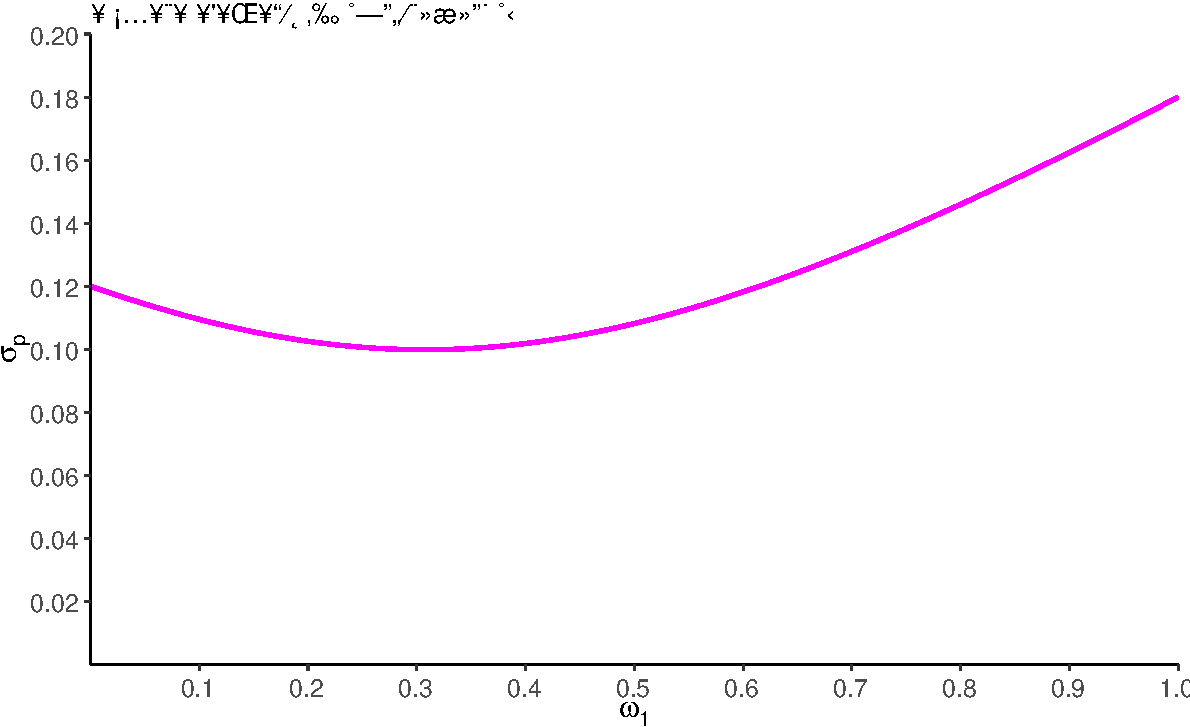
\includegraphics[keepaspectratio]{Hatakeda_Chap02_files/figure-pdf/unnamed-chunk-4-1.pdf}}

\section{確率変数}\label{ux78baux7387ux5909ux6570}

これまでの観測データの値から,TOPIX,とりわけTOPIXのリターンはランダムな(確率的な)値をとっていることが分かります。
つまり\textbf{予測不可能}なデータということです。
TOPIXの長期的な傾向(Trend)はある程度予想することは可能ですが,明日明後日のTOPIXの値といった短期的な動向を予測することはほぼ不可能です。
つまり,TOPIXやTOPIXのリターンは,ある定まった値というよりも,\textbf{不確実な値をとる変数}であると考えることができます。
このような変数を\textbf{確率変数}(random variables)とよびます。

\begin{tcolorbox}[enhanced jigsaw, colframe=quarto-callout-important-color-frame, breakable, rightrule=.15mm, coltitle=black, title=\textcolor{quarto-callout-important-color}{\faExclamation}\hspace{0.5em}{確率変数}, colbacktitle=quarto-callout-important-color!10!white, leftrule=.75mm, colback=white, left=2mm, arc=.35mm, opacityback=0, titlerule=0mm, toptitle=1mm, bottomtitle=1mm, bottomrule=.15mm, toprule=.15mm, opacitybacktitle=0.6]

ある試行(trial)によって起こりうる事象\(\omega\)に対して,ある実数値\(x = X(\omega)\)が与えられ,それぞれの値が起こりうる確率密度関数\(p(x)\)が与えられる場合,\(\omega\)から\(x\)への関数\(X:\omega \mapsto x\)を\textbf{確率変数}(random
variable)とよびます。
確率変数という名前がついていますが,実は関数なのです。

\end{tcolorbox}

\begin{tcolorbox}[enhanced jigsaw, colframe=quarto-callout-tip-color-frame, breakable, rightrule=.15mm, coltitle=black, title=\textcolor{quarto-callout-tip-color}{\faLightbulb}\hspace{0.5em}{例:コイン投げ}, colbacktitle=quarto-callout-tip-color!10!white, leftrule=.75mm, colback=white, left=2mm, arc=.35mm, opacityback=0, titlerule=0mm, toptitle=1mm, bottomtitle=1mm, bottomrule=.15mm, toprule=.15mm, opacitybacktitle=0.6]

1枚のコインを投げるという試行から起こりうる事象を\(\boldsymbol{H}\)と\(\boldsymbol{T}\)で表わします。

\begin{itemize}
\tightlist
\item
  \textbf{試行}(trial):コイン投げ
\item
  \textbf{起こりうる結果}(事象):\(\omega =\boldsymbol{H}, \boldsymbol{T}\)の2つの事象が起こりうる。
\item
  \textbf{試行の結果}:\(\boldsymbol{H}\)の数\(x = \{X(\boldsymbol{H}), X(\boldsymbol{T}) \} = \{ 1,0 \}\)
\item
  \textbf{各結果が起こる確率}:\(p(1) = p(0) = 0.5\)
\end{itemize}

\end{tcolorbox}

実現した\(\boldsymbol{H}\)の数(つまり表が出た回数)を\(x\)とするとき,事象\(\omega\)から\(x\)への関数\(X\)(コイン投げによる\textbf{表の数})は確率変数である。

厳密な表現は分かりにくいですね\ldots。
直感的には,確率を持った変数として理解してください。
でも,しばらく厳密にいきましょう!

\begin{Shaded}
\begin{Highlighting}[]
\KeywordTok{\textbackslash{}begin}\NormalTok{\{}\ExtensionTok{tikzpicture}\NormalTok{\}}
\FunctionTok{\textbackslash{}draw}\NormalTok{ (0,1) node [left]\{}\SpecialStringTok{$X$}\NormalTok{\};}
\FunctionTok{\textbackslash{}draw}\NormalTok{ (0,3) node \{before coin toss\};}
\FunctionTok{\textbackslash{}draw}\NormalTok{ (4,3) node \{after coin toss\};}
\FunctionTok{\textbackslash{}draw}\NormalTok{ [thick, {-}\textgreater{}] (0,1) {-}{-} (4,2) node[pos=0.5, sloped, above]\{}\SpecialStringTok{$p(1)=0.5$}\NormalTok{\};}
\FunctionTok{\textbackslash{}draw}\NormalTok{ (4,2) node [right] \{}\SpecialStringTok{$}\SpecialCharTok{\textbackslash{}omega}\SpecialStringTok{ = }\SpecialCharTok{\textbackslash{}boldsymbol}\SpecialStringTok{\{H\}, x=1$}\NormalTok{\};}
\FunctionTok{\textbackslash{}draw}\NormalTok{ [thick, {-}\textgreater{}] (0,1) {-}{-} (4,0) node[pos=0.5, sloped, below]\{}\SpecialStringTok{$p(0)=0.5$}\NormalTok{\};}
\FunctionTok{\textbackslash{}draw}\NormalTok{ (4,0) node [right] \{}\SpecialStringTok{$}\SpecialCharTok{\textbackslash{}omega}\SpecialStringTok{ = }\SpecialCharTok{\textbackslash{}boldsymbol}\SpecialStringTok{\{T\}, x=0$}\NormalTok{\};}
\KeywordTok{\textbackslash{}end}\NormalTok{\{}\ExtensionTok{tikzpicture}\NormalTok{\}}
\end{Highlighting}
\end{Shaded}

\begin{figure}[H]

{\centering 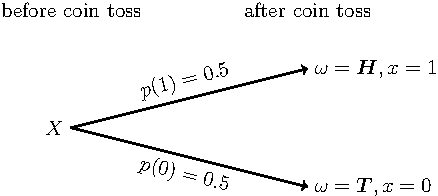
\includegraphics[width=0.9\linewidth,height=\textheight,keepaspectratio]{Hatakeda_Chap02_files/figure-pdf/tikz-example-1.pdf}

}

\caption{コイン投げの例}

\end{figure}%

確率は対応する値がどのくらいの割合で発生するかを表します。

\begin{Shaded}
\begin{Highlighting}[]
\NormalTok{df }\OtherTok{\textless{}{-}} \FunctionTok{data.frame}\NormalTok{(}
\NormalTok{  coin }\OtherTok{\textless{}{-}} \FunctionTok{c}\NormalTok{(}\StringTok{"H"}\NormalTok{, }\StringTok{"T"}\NormalTok{),}
\NormalTok{  p }\OtherTok{\textless{}{-}} \FunctionTok{c}\NormalTok{(}\FloatTok{0.5}\NormalTok{, }\FloatTok{0.5}\NormalTok{)}
\NormalTok{)}
\NormalTok{g }\OtherTok{\textless{}{-}} \FunctionTok{ggplot}\NormalTok{(df) }\SpecialCharTok{+} \FunctionTok{aes}\NormalTok{(}\AttributeTok{x =}\NormalTok{ coin, }\AttributeTok{y =}\NormalTok{ p) }\SpecialCharTok{+} \FunctionTok{geom\_col}\NormalTok{()}
\NormalTok{g }\OtherTok{\textless{}{-}}\NormalTok{ g }\SpecialCharTok{+} \FunctionTok{ylim}\NormalTok{(}\DecValTok{0}\NormalTok{,}\DecValTok{1}\NormalTok{) }\SpecialCharTok{+} \FunctionTok{xlab}\NormalTok{(}\StringTok{"確率"}\NormalTok{) }\SpecialCharTok{+} \FunctionTok{ylab}\NormalTok{(}\StringTok{"結果"}\NormalTok{)}
\FunctionTok{print}\NormalTok{(g)}
\end{Highlighting}
\end{Shaded}

\pandocbounded{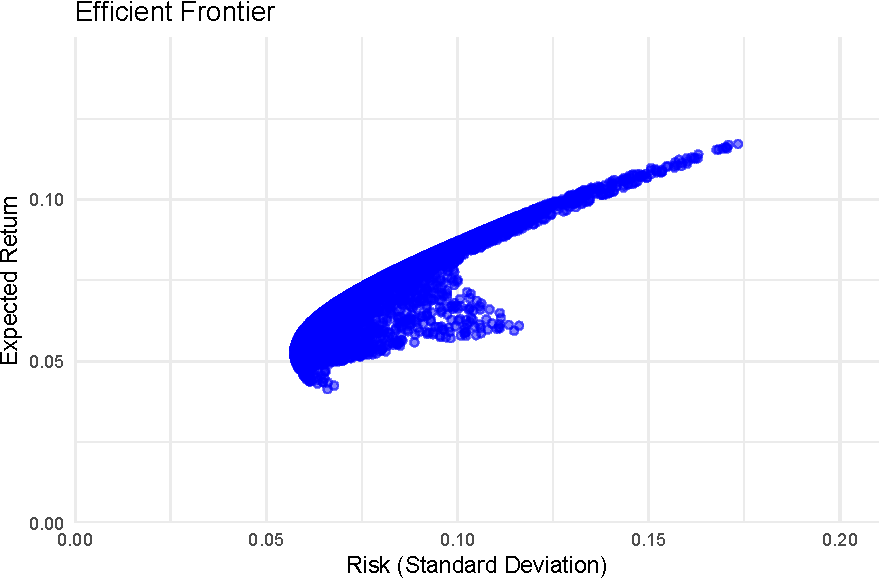
\includegraphics[keepaspectratio]{Hatakeda_Chap02_files/figure-pdf/unnamed-chunk-5-1.pdf}}

\begin{tcolorbox}[enhanced jigsaw, colframe=quarto-callout-note-color-frame, breakable, rightrule=.15mm, coltitle=black, title=\textcolor{quarto-callout-note-color}{\faInfo}\hspace{0.5em}{2枚コイン投げの例}, colbacktitle=quarto-callout-note-color!10!white, leftrule=.75mm, colback=white, left=2mm, arc=.35mm, opacityback=0, titlerule=0mm, toptitle=1mm, bottomtitle=1mm, bottomrule=.15mm, toprule=.15mm, opacitybacktitle=0.6]

\begin{itemize}
\tightlist
\item
  \textbf{試行} (trial) : コイン投げ
\item
  \textbf{起こりうる事象} : \$\omega = \{ (H,H),(H,T),(T,H),(T,T)\} \$
\item
  \textbf{試行結果} : 表の数
  \(x = \{ X(H,H),X(H,T),X(T,H),X(T,T)\} = \{2,1,0\}\)
\item
  \textbf{各結果が起こる確率} : \(p(2) = 0.25\),\(p(1) = 0.25\)
  ,\(p(0) = 0.25\)
\end{itemize}

表の数を\(x\)とするとき,\(\omega\)から\(x\)への関数\(X:\omega \mapsto x\)(2枚のコイン投げによる表の数)は確率変数です。

\end{tcolorbox}

\begin{Shaded}
\begin{Highlighting}[]
\KeywordTok{\textbackslash{}begin}\NormalTok{\{}\ExtensionTok{tikzpicture}\NormalTok{\}}
\FunctionTok{\textbackslash{}draw}\NormalTok{ (0,2) node [left]\{}\SpecialStringTok{$X$}\NormalTok{\};}
\FunctionTok{\textbackslash{}draw}\NormalTok{ (0,5) node \{before coin toss\};}
\FunctionTok{\textbackslash{}draw}\NormalTok{ (4,5) node \{after coin toss\};}
\FunctionTok{\textbackslash{}draw}\NormalTok{ [thick, {-}\textgreater{}] (0,2) {-}{-} (4,4) node[pos=0.5, sloped,  above]\{}\SpecialStringTok{$p(2)=0.25$}\NormalTok{\};}
\FunctionTok{\textbackslash{}draw}\NormalTok{ (4,4) node [right] \{}\SpecialStringTok{$}\SpecialCharTok{\textbackslash{}omega}\SpecialStringTok{ = (}\SpecialCharTok{\textbackslash{}boldsymbol}\SpecialStringTok{\{H\},}\SpecialCharTok{\textbackslash{}boldsymbol}\SpecialStringTok{\{H\}), x=2$}\NormalTok{\};}
\FunctionTok{\textbackslash{}draw}\NormalTok{ [thick, {-}\textgreater{}] (0,2) {-}{-} (4,2) node[pos=0.5, above]\{}\SpecialStringTok{$p(1)=0.5$}\NormalTok{\};}
\FunctionTok{\textbackslash{}draw}\NormalTok{ (4,2) node [right] \{}\SpecialStringTok{$}\SpecialCharTok{\textbackslash{}omega}\SpecialStringTok{ = (}\SpecialCharTok{\textbackslash{}boldsymbol}\SpecialStringTok{\{H\},}\SpecialCharTok{\textbackslash{}boldsymbol}\SpecialStringTok{\{T\}), x=1$}\NormalTok{\};}
\FunctionTok{\textbackslash{}draw}\NormalTok{ [thick, {-}\textgreater{}] (0,2) {-}{-} (4,0) node[pos=0.5, sloped, below]\{}\SpecialStringTok{$p(0)=0.25$}\NormalTok{\};}
\FunctionTok{\textbackslash{}draw}\NormalTok{ (4,0) node [right] \{}\SpecialStringTok{$}\SpecialCharTok{\textbackslash{}omega}\SpecialStringTok{ = (}\SpecialCharTok{\textbackslash{}boldsymbol}\SpecialStringTok{\{T\},}\SpecialCharTok{\textbackslash{}boldsymbol}\SpecialStringTok{\{T\}), x=0$}\NormalTok{\};}
\KeywordTok{\textbackslash{}end}\NormalTok{\{}\ExtensionTok{tikzpicture}\NormalTok{\}}
\end{Highlighting}
\end{Shaded}

\begin{figure}[H]

{\centering \includegraphics[width=0.9\linewidth,height=\textheight,keepaspectratio]{Hatakeda_Chap02_files/figure-pdf/unnamed-chunk-6-1.pdf}

}

\caption{コイン投げの例}

\end{figure}%

\begin{Shaded}
\begin{Highlighting}[]
\NormalTok{df }\OtherTok{\textless{}{-}} \FunctionTok{data.frame}\NormalTok{(}
\NormalTok{  coin }\OtherTok{\textless{}{-}} \FunctionTok{c}\NormalTok{(}\StringTok{"HH"}\NormalTok{, }\StringTok{"HT"}\NormalTok{,}\StringTok{"TT"}\NormalTok{),}
\NormalTok{  p }\OtherTok{\textless{}{-}} \FunctionTok{c}\NormalTok{(}\FloatTok{0.25}\NormalTok{, }\FloatTok{0.5}\NormalTok{,}\FloatTok{0.25}\NormalTok{)}
\NormalTok{)}
\NormalTok{g }\OtherTok{\textless{}{-}} \FunctionTok{ggplot}\NormalTok{(df) }\SpecialCharTok{+} \FunctionTok{aes}\NormalTok{(}\AttributeTok{x =}\NormalTok{ coin, }\AttributeTok{y =}\NormalTok{ p) }\SpecialCharTok{+} \FunctionTok{geom\_col}\NormalTok{()}
\NormalTok{g }\OtherTok{\textless{}{-}}\NormalTok{ g }\SpecialCharTok{+} \FunctionTok{ylim}\NormalTok{(}\DecValTok{0}\NormalTok{,}\DecValTok{1}\NormalTok{) }\SpecialCharTok{+} \FunctionTok{xlab}\NormalTok{(}\StringTok{"確率"}\NormalTok{) }\SpecialCharTok{+} \FunctionTok{ylab}\NormalTok{(}\StringTok{"結果"}\NormalTok{)}
\FunctionTok{print}\NormalTok{(g)}
\end{Highlighting}
\end{Shaded}

\pandocbounded{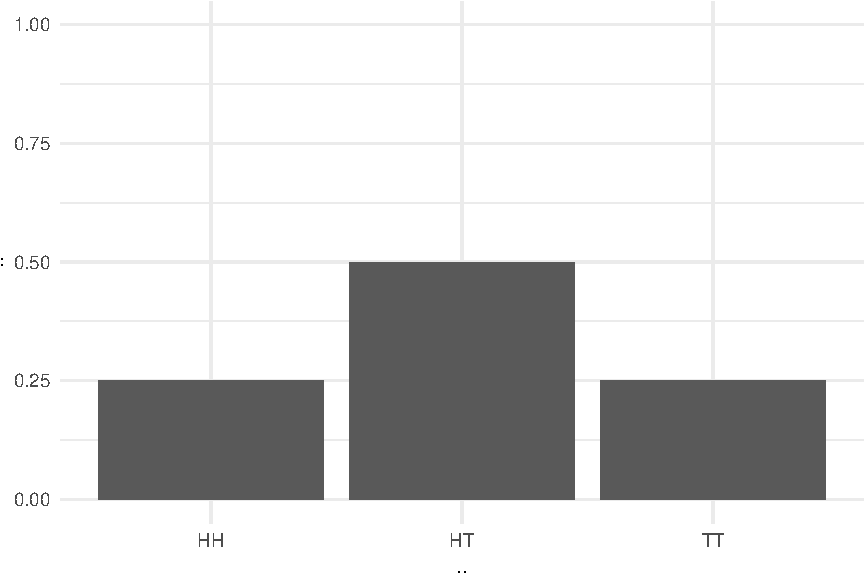
\includegraphics[keepaspectratio]{Hatakeda_Chap02_files/figure-pdf/unnamed-chunk-7-1.pdf}}

先の例と同様に、各確率の対応する値がどれくらいの割合で発生するかを表しています。
この確率分布は確率変数の特徴を表しています。

\begin{tcolorbox}[enhanced jigsaw, colframe=quarto-callout-warning-color-frame, breakable, rightrule=.15mm, coltitle=black, title=\textcolor{quarto-callout-warning-color}{\faExclamationTriangle}\hspace{0.5em}{練習問題}, colbacktitle=quarto-callout-warning-color!10!white, leftrule=.75mm, colback=white, left=2mm, arc=.35mm, opacityback=0, titlerule=0mm, toptitle=1mm, bottomtitle=1mm, bottomrule=.15mm, toprule=.15mm, opacitybacktitle=0.6]

コインを4枚投げたときに出た表の数を\(x\)で表すとします。
このとき,以下の(1)〜(4)について答えなさい。

\begin{enumerate}
\def\labelenumi{\arabic{enumi}.}
\tightlist
\item
  起こりうる事象
\item
  試行結果
\item
  各結果が起こる確率
\item
  確率分布
\end{enumerate}

\end{tcolorbox}

確率変数により,われわれは\textbf{不確実性}を伴う現象を記述できるようになりました。
確率変数という用語は,結果を観測する\textbf{前}の状況を指し示しています。
まとめると、

\begin{itemize}
\tightlist
\item
  これからどうなるかを表しているのが確率変数です。
\item
  試行後において,確率変数がとって具体的な\(x\)の値は実現値(realized
  value)といいます。
\item
  確率変数に2つの側面(観測前と観測後)があり,これらを区別する必要があります。
\item
  確率変数\(X\)が取りうる値\(x\)に応じて,

  \begin{itemize}
  \tightlist
  \item
    \textbf{離散型確率変数}(discrete random variables)
  \item
    \textbf{連続型確率変数}(continuous random variables)
  \end{itemize}

  に区別することができます。
\end{itemize}

当面は,\textbf{離散型確率変数}に着目します。

(金融)資産を購入をする際,われわれはその資産を将来価値を確認した上で,購入の意思決定をしているのではありません。
その資産について将来においてどのような値が実現するのか知らないうちに,購入の意思決定を行います。
つまり,資産の価値は不確実性を伴う,したがって資産の価値は確率変数である。
このとき,どのようなことを考慮して購入の意思決定を行うのか?

意思決定者は,不確実性に直面しているとき,実現するかもしれない特定の値よりも,実現する値の\textbf{起こりやすさ},つまり\textbf{確率分布}に関心を持っている。
一般に,確率分布の特徴の中でも,中心とばらつきに関心を持つ傾向がある。
確率分布を意識しない人,具体的には宝くじの賞金(景品)にのみ関心をもつような人はたいてい失敗する結末が!!

先に示した確率分布の特徴(中心とばらつき)は,指標として統計学的に定義されています。

\begin{tcolorbox}[enhanced jigsaw, colframe=quarto-callout-important-color-frame, breakable, rightrule=.15mm, coltitle=black, title=\textcolor{quarto-callout-important-color}{\faExclamation}\hspace{0.5em}{期待値}, colbacktitle=quarto-callout-important-color!10!white, leftrule=.75mm, colback=white, left=2mm, arc=.35mm, opacityback=0, titlerule=0mm, toptitle=1mm, bottomtitle=1mm, bottomrule=.15mm, toprule=.15mm, opacitybacktitle=0.6]

\textbf{期待値}(expectation)とは、確率変数\(X\)がとりうる値の加重平均であり、確率分布の\textbf{中心の位置}を表します。
起こりうる値を\(x_k\),その確率を\(p_k\)とすると,確率変数\(X\)の期待値の公式は以下ようになります。
\[
\begin{aligned}
\mathbb{E} [X] := \sum _{k} p_k x_k
\end{aligned}
\]

\end{tcolorbox}

\begin{tcolorbox}[enhanced jigsaw, colframe=quarto-callout-important-color-frame, breakable, rightrule=.15mm, coltitle=black, title=\textcolor{quarto-callout-important-color}{\faExclamation}\hspace{0.5em}{分散}, colbacktitle=quarto-callout-important-color!10!white, leftrule=.75mm, colback=white, left=2mm, arc=.35mm, opacityback=0, titlerule=0mm, toptitle=1mm, bottomtitle=1mm, bottomrule=.15mm, toprule=.15mm, opacitybacktitle=0.6]

\textbf{分散}(variance)とは、確率変数\(X\)がとりうる値と期待値との乖離の期待値であり,確率分布の\textbf{ばらつきの程度}を表します。
確率変数\(X\)の分散の公式は以下ようになります。 \[
\begin{aligned}
\mathbb{V} [X] &:= \mathbb{E} \left [ (X - \mathbb{E} [X])^2 \right ] \\
&=  \sum _{k} p_k ( x_k - \mathbb{E}[X] )^2
\end{aligned}
\]

\end{tcolorbox}

\begin{tcolorbox}[enhanced jigsaw, colframe=quarto-callout-important-color-frame, breakable, rightrule=.15mm, coltitle=black, title=\textcolor{quarto-callout-important-color}{\faExclamation}\hspace{0.5em}{標準偏差}, colbacktitle=quarto-callout-important-color!10!white, leftrule=.75mm, colback=white, left=2mm, arc=.35mm, opacityback=0, titlerule=0mm, toptitle=1mm, bottomtitle=1mm, bottomrule=.15mm, toprule=.15mm, opacitybacktitle=0.6]

\textbf{標準偏差}(standard
deviation)は分散の平方根であり,次のように定義されます。 \[
\begin{aligned}
\sigma [X] := \sqrt{\mathbb{V}[X]}
\end{aligned}
\]

\end{tcolorbox}

先に示した確率分布の特徴は,分布の中心である期待値と,ばらつきの程度である分散(あるいは標準偏差)で表現されます。
ばらつきの程度の指標である分散は,不確実性の程度を表しており,ファイナンスでは\textbf{リスク}(risk)とよびます。
重要なことですが、上で説明した期待値,分散,標準偏差といった指標はパラメータ(定数)であり,確率変数ではありません。

\begin{tcolorbox}[enhanced jigsaw, colframe=quarto-callout-tip-color-frame, breakable, rightrule=.15mm, coltitle=black, title=\textcolor{quarto-callout-tip-color}{\faLightbulb}\hspace{0.5em}{例5:資産投資}, colbacktitle=quarto-callout-tip-color!10!white, leftrule=.75mm, colback=white, left=2mm, arc=.35mm, opacityback=0, titlerule=0mm, toptitle=1mm, bottomtitle=1mm, bottomrule=.15mm, toprule=.15mm, opacitybacktitle=0.6]

投資資産\(A\)と\(B\)を運用して得られるリターンが以下の通りとします。

\begin{longtable}[]{@{}cccccc@{}}
\toprule\noalign{}
投資資産A & & & & & \\
\midrule\noalign{}
\endhead
\bottomrule\noalign{}
\endlastfoot
状態 & 1 & 2 & 3 & 4 & 5 \\
確率 & \(40\%\) & \(20\%\) & \(20\%\) & \(10\%\) & \(10\%\) \\
リターン & \(-100\%\) & \(-75\%\) & \(-50\%\) & \(-25\%\) &
\(1000\%\) \\
\end{longtable}

\begin{longtable}[]{@{}cccccc@{}}
\toprule\noalign{}
投資資産B & & & & & \\
\midrule\noalign{}
\endhead
\bottomrule\noalign{}
\endlastfoot
状態 & 1 & 2 & 3 & 4 & 5 \\
確率 & \(40\%\) & \(20\%\) & \(20\%\) & \(10\%\) & \(10\%\) \\
リターン & \(-15\%\) & \(0\%\) & \(15\%\) & \(10\%\) & \(25\%\) \\
\end{longtable}

\begin{longtable}[]{@{}lrr@{}}
\toprule\noalign{}
& 投資資産A & 投資資産B \\
\midrule\noalign{}
\endhead
\bottomrule\noalign{}
\endlastfoot
\(\mathbb{E}[X]\) & \(32.5\) & \(0.5\) \\
\(\mathbb{SD}[X]\) & \(323.5\) & \(14.4\) \\
\end{longtable}

\end{tcolorbox}

\begin{tcolorbox}[enhanced jigsaw, colframe=quarto-callout-warning-color-frame, breakable, rightrule=.15mm, coltitle=black, title=\textcolor{quarto-callout-warning-color}{\faExclamationTriangle}\hspace{0.5em}{練習問題}, colbacktitle=quarto-callout-warning-color!10!white, leftrule=.75mm, colback=white, left=2mm, arc=.35mm, opacityback=0, titlerule=0mm, toptitle=1mm, bottomtitle=1mm, bottomrule=.15mm, toprule=.15mm, opacitybacktitle=0.6]

上記設定のもとで、2つの資産が生み出すリターンの期待値と分散を求めてください。

\begin{longtable}[]{@{}ccc@{}}
\toprule\noalign{}
& 資産\(A\) & 資産\(B\) \\
\midrule\noalign{}
\endhead
\bottomrule\noalign{}
\endlastfoot
\(\mathbb{E}[X]\) & \(32.5\) & (\(\quad\)) \\
\(\mathbb{V}[X]\) & \(323.5\) & (\(\quad\)) \\
\end{longtable}

\end{tcolorbox}

\begin{tcolorbox}[enhanced jigsaw, colframe=quarto-callout-warning-color-frame, breakable, rightrule=.15mm, coltitle=black, title=\textcolor{quarto-callout-warning-color}{\faExclamationTriangle}\hspace{0.5em}{解答}, colbacktitle=quarto-callout-warning-color!10!white, leftrule=.75mm, colback=white, left=2mm, arc=.35mm, opacityback=0, titlerule=0mm, toptitle=1mm, bottomtitle=1mm, bottomrule=.15mm, toprule=.15mm, opacitybacktitle=0.6]

定義通りに、投資資産\(A\)の期待値と分散を求めます。

\begin{longtable}[]{@{}ccc@{}}
\toprule\noalign{}
& 資産\(A\) & 資産\(B\) \\
\midrule\noalign{}
\endhead
\bottomrule\noalign{}
\endlastfoot
\(\mathbb{E}[X]\) & \(32.5\) & (\(\quad\)) \\
\(\mathbb{V}[X]\) & \(323.5\) & (\(\quad\)) \\
\end{longtable}

\[
\begin{aligned}
\mathbb{E}[A] &= 0.4 \times (-100) + 0.2 \times (-75) + 0.2 \times (-50) \\
&+ 0.1 \times (-25) + 0.1 \times 1000\\
       &= 32.50\% \\
\mathbb{V}[A]&= 0.4(-100 - 32.5)^2 + 0.2(-75 - 32.5)^2 + 0.2(-50 - 32.5)^2 \\
&+ 0.1(-25 - 32.5)^2 + 0.1(1000 - 32.5)^2 \\
        &= 104631.25\\
\sigma[A] & = \sqrt{104631.25} = 323.47\%
\end{aligned}
\]

\end{tcolorbox}

\subsection{2つの確率変数どうしの関係}\label{ux3064ux306eux78baux7387ux5909ux6570ux3069ux3046ux3057ux306eux95a2ux4fc2}

2つの確率変数の関連性は,共分散と相関係数で表します。
以下では、それぞれの定義とともに、その統計量の特徴を説明します。

\begin{tcolorbox}[enhanced jigsaw, colframe=quarto-callout-important-color-frame, breakable, rightrule=.15mm, coltitle=black, title=\textcolor{quarto-callout-important-color}{\faExclamation}\hspace{0.5em}{共分散}, colbacktitle=quarto-callout-important-color!10!white, leftrule=.75mm, colback=white, left=2mm, arc=.35mm, opacityback=0, titlerule=0mm, toptitle=1mm, bottomtitle=1mm, bottomrule=.15mm, toprule=.15mm, opacitybacktitle=0.6]

確率変数\(X_i\)と\(X_j\)との\textbf{共分散}(covariance)を\(\mathbb{COV}[X_i,X_j]\)で表す。
\[
\begin{aligned}
\mathbb{COV} [X_i,X_j] &= \sigma _{ij} \\
&= \mathbb{E} \left[ (X_i - \mathbb{E}[X_i])(X_j - \mathbb{E}[X_j]) \right]\\
&= \sum _k p_k (x_{i,k} - \mathbb{E} [X_i])(x_{j,k} - \mathbb{E} [X_j])
\end{aligned}
\]

\end{tcolorbox}

定義より,\(i=j\)のとき,\(\mathbb{COV} [X_i,X_j] = \mathbb{V}[X_i]\)となります。
つまり分散は共分散の特殊ケース(\(i=j\)のケース)となります。

\begin{tcolorbox}[enhanced jigsaw, colframe=quarto-callout-important-color-frame, breakable, rightrule=.15mm, coltitle=black, title=\textcolor{quarto-callout-important-color}{\faExclamation}\hspace{0.5em}{相関係数}, colbacktitle=quarto-callout-important-color!10!white, leftrule=.75mm, colback=white, left=2mm, arc=.35mm, opacityback=0, titlerule=0mm, toptitle=1mm, bottomtitle=1mm, bottomrule=.15mm, toprule=.15mm, opacitybacktitle=0.6]

2変数の関係を表すもう1つの尺度が\textbf{相関係数}(correlation)です。
\(X_i\)と\(X_j\)との相関係数を\(\rho _{ij}\)で表すとします。なぜか伝統的にギリシャ文字のロー\(\rho\)で相関係数を表すことが多いので覚えておきましょう。
相関係数は,2つの変数の共分散をそれぞれの標準偏差の積で除した値です。こうすることで,共分散の値が変数の単位に依存しない値となります。

\[
\begin{aligned}
\rho _{ij} \equiv \frac{\mathbb{COV}[X_i,X_j]}{\sigma [X_i] \sigma [X_j]}
\end{aligned}
\]

\begin{itemize}
\tightlist
\item
  相関係数は,\(-1 \leq \rho _{ij} \leq 1\)の値をとります。
\item
  相関係数は,\(X_i\)と\(X_j\)との\textbf{線形関係の程度}を表します
\item
  相関係数の符号を決定づけるのは,\(\mathbb{COV}[X_i, X_j]\)の符号です。
\item
  相関係数の大きさは,共分散の大きさだけでなく,\(\sigma [X_i]\)と\(\sigma [X_j]\)の大きさに依存します。
\end{itemize}

\end{tcolorbox}

\begin{tcolorbox}[enhanced jigsaw, colframe=quarto-callout-warning-color-frame, breakable, rightrule=.15mm, coltitle=black, title=\textcolor{quarto-callout-warning-color}{\faExclamationTriangle}\hspace{0.5em}{問題2:投資資産}, colbacktitle=quarto-callout-warning-color!10!white, leftrule=.75mm, colback=white, left=2mm, arc=.35mm, opacityback=0, titlerule=0mm, toptitle=1mm, bottomtitle=1mm, bottomrule=.15mm, toprule=.15mm, opacitybacktitle=0.6]

上記の投資資産の数値例に基づいて,投資資産\(A\)と\(B\)の共分散および相関係数を求めよ。

\begin{itemize}
\tightlist
\item
  \(\sigma _{AB}\)
\item
  \(\rho _{AB}\)
\end{itemize}

\end{tcolorbox}

\section{演算規則}\label{ux6f14ux7b97ux898fux5247}

\subsection{期待値の演算規則}\label{ux671fux5f85ux5024ux306eux6f14ux7b97ux898fux5247}

期待値の演算について,次のような法則が成り立っています。
重要な法則ですので、一つ一つ確認しながら理解するようにしてください。

まず,\(X\)が確率変数ではなく,定数・パラメータであるとき, \[
\begin{aligned}
\mathbb{E} [X] = X
\end{aligned}
\]

たとえば,

\[
\begin{aligned}
\mathbb{E} [10] = 10
\end{aligned}
\]

同様に,\(a\)がパラメータや代表値(期待値,分散,標準偏差)であるとき,

\[
\begin{aligned}
\mathbb{E} [a] &= a\\
\mathbb{E} [ \mathbb{E}[X]] &= \mathbb{E}[X]\\
\mathbb{E} [\mathbb{V} [X]] &= \mathbb{V}[X]
\end{aligned}
\]

となります。

次に、\(X\)が確率変数であり,\(b\)がパラメータであるとき, \[
\begin{aligned}
\mathbb{E} [bX] &= b \mathbb{E}[X] \\
\mathbb{E} [\mathbb{E}[X] X] &= \mathbb{E}[X] \times \mathbb{E}[X] = \mathbb{E}[X]^2
\end{aligned}
\]

パラメータは期待値の外に出すことができます。 したがって,

\[
\begin{aligned}
\mathbb{E} [X]^2 \not = \mathbb{E} [X^2]
\end{aligned}
\]

\(X\)と\(Y\)が確率変数であるとき,

\[
\begin{aligned}
\mathbb{E}[X+Y] = \mathbb{E} [X] + \mathbb{E} [Y]
\end{aligned}
\]

のように,期待値を分解することができます。

\(a\)が確定変数であり,\(X\)が確率変数であり,\(b\)がパラメータであるとき,

\[
\begin{aligned}
\mathbb{E} [a + bX] = \mathbb{E} [a] + \mathbb{E} [bX] = a + b \mathbb{E}[X]
\end{aligned}
\]

が成り立ちます。

\subsection{分散の演算規則}\label{ux5206ux6563ux306eux6f14ux7b97ux898fux5247}

\(X\)が確率変数ではなく,確定変数であるとき,

\[
\begin{aligned}
\mathbb{V}[X] = 0
\end{aligned}
\]

\begin{tcolorbox}[enhanced jigsaw, colframe=quarto-callout-warning-color-frame, breakable, rightrule=.15mm, coltitle=black, title=\textcolor{quarto-callout-warning-color}{\faExclamationTriangle}\hspace{0.5em}{証明}, colbacktitle=quarto-callout-warning-color!10!white, leftrule=.75mm, colback=white, left=2mm, arc=.35mm, opacityback=0, titlerule=0mm, toptitle=1mm, bottomtitle=1mm, bottomrule=.15mm, toprule=.15mm, opacitybacktitle=0.6]

分散の定義は \[
\begin{aligned}
\mathbb{V}[X] = \sum _k p_k (x_i - \mathbb{E}[X])
\end{aligned}
\]

です。いま\(X\)が確定変数であるため,\(x_i = X\)かつ\(\mathbb{E}[X] = X\)となります。
つまり\(\mathbb{V}[X] = 0\)となります。

\end{tcolorbox}

同様に,\(a\)がパラメータや代表値(期待値・分散・標準偏差)であるとき, \[
\begin{aligned}
\mathbb{V} [a] &= 0 , & \mathbb{V} [\mathbb{E}[X]] &= 0,&  \mathbb{V}[\mathbb{V}[X]] &= 0
\end{aligned}
\] が成立する。

\(X\)が確率変数であり,\(b\)が定数やパラメータであるとき, \[
\begin{aligned}
\mathbb{V}[bX] &\equiv \mathbb{E} \left [(bX -E[bx])^2 \right ] \qquad \Leftarrow \mathbb{E}[bX] = b\mathbb{E}[X] \nonumber \\
         &= \mathbb{E} \left[(bX - b \mathbb{E}[X])^2\right ]\nonumber \\
         &= \mathbb{E} \left[b^2 (X-\mathbb{E}[X])^2\right ] \qquad \Leftarrow \mathbb{E}[bX] = b\mathbb{E}[X]\nonumber \\
         &= b^2 \mathbb{E} \left[(X-\mathbb{E}[X])^2\right ] \qquad \Leftarrow \mathbb{V} [X] = \mathbb{E} \left [(X-\mathbb{E}[X])^2 \right ]\nonumber \\
         &= b^2 \mathbb{V} [X]
\end{aligned}
\]

となります。
パラメータは分散の外に出すことができるが,期待値のケースと異なり二乗されます。

\[
\begin{aligned}
\mathbb{V}[X] &\equiv \mathbb{E} \left [ (X - \mathbb{E} [X])^2 \right ] \nonumber  \\
        &=\mathbb{E} \left [ X^2 - 2X\mathbb{E}[X] + \mathbb{E}[X]^2 \right ] \qquad \Leftarrow \text{(9)式を適用し,期待値を分解}\nonumber \\
        &=\mathbb{E} \left [ X^2 \right ] - \mathbb{E} \left [ 2 X \mathbb{E}[X] \right ] + \mathbb{E} \left [ \mathbb{E}[X]^2 \right ]\nonumber \\
        &=\mathbb{E} \left [ X^2 \right ] - 2 X \mathbb{E} [X] \mathbb{E}[X] + \mathbb{E} [X]^2\nonumber \\
        &=\mathbb{E} \left [ X^2 \right ] - \mathbb{E} [X]^2
\end{aligned}
\]

\subsection{共分散の演算規則}\label{ux5171ux5206ux6563ux306eux6f14ux7b97ux898fux5247}

共分散については,以下の法則が成り立ちます。

\[
\begin{aligned}
\mathbb{COV}[X_i,X_j] = \sigma _{ij} &\equiv \mathbb{E}  \left [(X_i - \mathbb{E}[X_i])(X_j - \mathbb{E}[X_j]) \right ] \nonumber \\
&= \mathbb{E}[X_i X_j - X_i \mathbb{E}[X_j] - \mathbb{E}[X_i]X_j + \mathbb{E}[X_i]\mathbb{E}[X_j]]\nonumber \\
&= \mathbb{E}[X_i X_j] - \mathbb{E}[X_i \mathbb{E}[X_j]] - \mathbb{E}[\mathbb{E}[X_i]X_j] + \mathbb{E}[\mathbb{E}[X_i]\mathbb{E}[X_j]]\nonumber  \\
&= \mathbb{E}[X_i X_j] - \mathbb{E}[X_i] \mathbb{E}[X_j] - \mathbb{E}[X_i]\mathbb{E}[X_j] + \mathbb{E}[X_i]\mathbb{E}[X_j] \nonumber \\
&= \mathbb{E}[X_i X_j] - \mathbb{E}[X_i] \mathbb{E}[X_j]
\end{aligned}
\]

\(\mathbb{COV}[X_i,X_j]=0\)つまり無相関であるなら,次の関係が成り立つ。

\[
\begin{aligned}
\mathbb{E}[X_iX_j] = \mathbb{E}[X_i]\mathbb{E}[X_j]
\end{aligned}
\]

\section{確率変数のアフィン変換}\label{ux78baux7387ux5909ux6570ux306eux30a2ux30d5ux30a3ux30f3ux5909ux63db}

確率変数\(X\)がアフィン変換(affine transformation)をする場合を考えます。

\[
\begin{aligned}
Y = a + bX
\end{aligned}
\]

によって確率変数\(X\)が確率変数\(Y\)に変換されたとします。
ここで\(a\)と\(b\)はパラメータです。 このとき,次の関係が成立します。

まず期待値については

\[
\begin{aligned}
\mathbb{E}[Y] &= \mathbb{E}[a + bX] \nonumber \\
       &= \mathbb{E}[a] + \mathbb{E}[bX] \nonumber\\
       &= a + b \mathbb{E}[X]
\end{aligned}
\] となり,分散については, \[
\begin{aligned}
\mathbb{V}[Y]
        &= \mathbb{E}[(Y - \mathbb{E}[Y])^2]      \nonumber \\
        &= \mathbb{E}[(a + bX - (a+b\mathbb{E}[X]))^2] \nonumber\\
        &= \mathbb{E}[(bX - b \mathbb{E}[X])^2]   \nonumber\\
        &= \mathbb{E}[b^2 (X - \mathbb{E}[X])^2]  \nonumber\\
        &= b^2 \mathbb{E}[ (X - \mathbb{E}[X])^2] \nonumber\\
        &= b^2 \mathbb{V}[X]
\end{aligned}
\]

となり,標準偏差については,

\[
\begin{aligned}
\sigma _Y = \sqrt{\mathbb{V}[Y]} = |b| \sqrt{\mathbb{V}[X]}
\end{aligned}
\]

となります。

\begin{tcolorbox}[enhanced jigsaw, colframe=quarto-callout-tip-color-frame, breakable, rightrule=.15mm, coltitle=black, title=\textcolor{quarto-callout-tip-color}{\faLightbulb}\hspace{0.5em}{アフィン変換}, colbacktitle=quarto-callout-tip-color!10!white, leftrule=.75mm, colback=white, left=2mm, arc=.35mm, opacityback=0, titlerule=0mm, toptitle=1mm, bottomtitle=1mm, bottomrule=.15mm, toprule=.15mm, opacitybacktitle=0.6]

ある工事が完了する日数とその確率が次のように予測されているとします。

\begin{longtable}[]{@{}cccccc@{}}
\toprule\noalign{}
日数\(X\) & 1 & 2 & 3 & 4 & 5 \\
\midrule\noalign{}
\endhead
\bottomrule\noalign{}
\endlastfoot
確率\(p(x)\) & \(5\%\) & \(20\%\) & \(35\%\) & \(30\%\) & \(10\%\) \\
\end{longtable}

このとき

\[
\begin{aligned}
\mathbb{E}[X] &\equiv \sum _k p_k x_k \text{より} & \mathbb{E}[X] &= 3.2\\
\mathbb{V} [X] &\equiv \sum _k p_k (x_k - \mathbb{E}[X])^2 \text{より} & \mathbb{V} [X] &= 1.06
\end{aligned}
\]

この工事では,固定費として100万円,変動費として1日あたり10万円の費用がかかるとすると,総費用は,

\[
\begin{aligned}
Y = 100  + 10 X
\end{aligned}
\]

として表される。 このとき,総費用の期待値および分散は,

\[
\begin{aligned}
\mathbb{E}[Y] &= 100 + 10 \mathbb{E}[X] = 100 + 10 \times 3.2 = 132\\
\mathbb{V}[Y] &= 10^2 \mathbb{V}[X] = 100  \times 1.06 = 106
\end{aligned}
\]

となる。

\end{tcolorbox}

より一般的に,\(k\)個の確率変数\(X_i\),
\(i = 1, \dots ,k\)の一次結合\(Y = c_0 + c_1 X_1 + \cdots + c_k X_k\)で表される確率変数\(Y\)において,次の関係が成立する。
ここで,\(c_0,c_1, \dots, c_k\)はパラメータで,定数です。

\[
\begin{aligned}
\mathbb{E}[Y] &= c_0 + c_1 \mu _1 + \cdots c_k \mu_k\\
\mathbb{V} [Y] &= c_1^2 \sigma_1^2 + \cdots +  c_k^2 \sigma _k^2 + \sum _{i\not = j}^k \sum_{j \not = i}^k c_i c_j \sigma _{ij}
\end{aligned}
\]

ここで,\(\mu _i = \mathbb{E}[X_i]\),\(\sigma _i^2 = \mathbb{V}[X_i]\),\(\sigma _{ij} = \mathbb{COV}[X_i,X_j]\)である。

例えば,\(k=2\)のケースでは,

\[
\begin{aligned}
\mathbb{E}[Y]   &= c_0 + c_1 \mu _1 + c_2 \mu_2\\
\mathbb{V} [Y] &= c_1^2 \sigma_1^2 + c_2^2 \sigma _2^2 + 2 c_1 c_2 \sigma _{12}
\end{aligned}
\]

\begin{tcolorbox}[enhanced jigsaw, colframe=quarto-callout-warning-color-frame, breakable, rightrule=.15mm, coltitle=black, title=\textcolor{quarto-callout-warning-color}{\faExclamationTriangle}\hspace{0.5em}{問題3}, colbacktitle=quarto-callout-warning-color!10!white, leftrule=.75mm, colback=white, left=2mm, arc=.35mm, opacityback=0, titlerule=0mm, toptitle=1mm, bottomtitle=1mm, bottomrule=.15mm, toprule=.15mm, opacitybacktitle=0.6]

\(k=3\)のケースにおける確率変数\(Y\)の期待値と分散を求めなさい。

\end{tcolorbox}

\begin{tcolorbox}[enhanced jigsaw, colframe=quarto-callout-warning-color-frame, breakable, rightrule=.15mm, coltitle=black, title=\textcolor{quarto-callout-warning-color}{\faExclamationTriangle}\hspace{0.5em}{例8}, colbacktitle=quarto-callout-warning-color!10!white, leftrule=.75mm, colback=white, left=2mm, arc=.35mm, opacityback=0, titlerule=0mm, toptitle=1mm, bottomtitle=1mm, bottomrule=.15mm, toprule=.15mm, opacitybacktitle=0.6]

\(k=2\)のケースで,\(Y=0.5X_1 + 0.5 X_2\)の期待値および分散を求めます。
ただし,\(\mu _1 = 0.07\),\(\sigma _1^2 = 1.48\),\(\mu_2 = -0.02\),\(\sigma _2^2 = 1.46\)とします。

\begin{itemize}
\item
  無相関(\(\rho _{12} = 0\), \(\mathbb{COV}[X_1, X_2] = 0\) )のケース \[
  \begin{aligned}
    \mathbb{E}[Y]   &= 0.5 \times 0.07 + 0.5 \times - 0.02 = 0.025\\
    \mathbb{V} [Y] &= 0.5^2 \times 1.48 + 0.5^2 \times 1.46 + 2 \times 0.5 \times 0.5 \times 0 = 0.735
    \end{aligned}
  \]

  \(Y\)の分散は,\(X_1\)と\(X_2\)の分散よりも小さい。
\item
  負の相関(\(\rho _{12} = -0.99 \Leftrightarrow \mathbb{COV}[X_1,X_2] = -1.46\))のケース
  \[
  \begin{aligned}
    \mathbb{E}[Y]   &= 0.5 \times 0.07 + 0.5 \times - 0.02 = 0.025\\
    \mathbb{V} [Y] &= 0.5^2 \times 1.48 + 0.5^2 \times 1.46 + 2 \times 0.5 \times 0.5 \times -1.46 = 0.005
    \end{aligned}
  \]

  \(Y\)の分散は,\(X_1\)と\(X_2\)の分散よりも小さい。
\end{itemize}

\(X_1\)と\(X_2\)の共分散は,\(Y\)の分散に影響を与える。

\end{tcolorbox}

\section{共分散の重要公式}\label{ux5171ux5206ux6563ux306eux91cdux8981ux516cux5f0f}

共分散について,以下の公式が成立する。

\[
\begin{aligned}
\mathbb{COV}[X, a + bY] & \equiv \mathbb{E}[(X - \mathbb{E}[X])](a+bY - \mathbb{E}[a + bY])\nonumber \\
                &= \mathbb{E}[(X - \mathbb{E}[X])(b(Y - \mathbb{E}[Y]))]\nonumber \\
                &= b \mathbb{E}[ (X - \mathbb{E}[X])(Y - \mathbb{E}[Y])]\nonumber \\
                &= b \mathbb{COV}[X,Y]
\end{aligned}
\]

同様に,上の式の発展系として,以下が成立する。

\[
\begin{aligned}
\mathbb{COV}[X_1, c_0 + c_1 X_1 + \cdots + c_k X_k] = c_1 \mathbb{V}[X_1] + \cdots + c_2\mathbb{COV}[X_1,X_2] + \cdots + c_k \mathbb{COV}[X_1,X_2]
\end{aligned}
\]

ここで,
\(\mathbb{COV}[X,X] = \mathbb{E}[ ( X - \mathbb{E}[X])(X- \mathbb{E}[X]) ] = \mathbb{V}[X]\)
であることを思い出そう。

\bookmarksetup{startatroot}

\chapter{統計}\label{ux7d71ux8a08}

前章で学習したように,ファイナンスではいろいろな理由から,資産価値それ自体より資産価値の\textbf{変化率},すなわち\textbf{リターン}(return)で議論することが多いです。
ここで,リターンの定義を再度確認します。

\begin{Shaded}
\begin{Highlighting}[]
\NormalTok{pacman}\SpecialCharTok{::}\FunctionTok{p\_load}\NormalTok{(tidyverse, ggthemes, patchwork, datasauRus, gganimate)}
\NormalTok{mystyle }\OtherTok{\textless{}{-}} \FunctionTok{list}\NormalTok{ (}\CommentTok{\#  ggplotのテーマ}
  \FunctionTok{theme\_few}\NormalTok{(),}
  \FunctionTok{theme}\NormalTok{(}
    \AttributeTok{text =} \FunctionTok{element\_text}\NormalTok{(}
      \AttributeTok{size=}\DecValTok{16}\NormalTok{,  }\CommentTok{\#  フォントサイズ}
     \AttributeTok{family =} \StringTok{"HiraKakuProN{-}W3"} \CommentTok{\# ヒラギノフォント}
\NormalTok{    )}
\NormalTok{  )}
\NormalTok{)}
\end{Highlighting}
\end{Shaded}

\begin{tcolorbox}[enhanced jigsaw, colframe=quarto-callout-important-color-frame, breakable, rightrule=.15mm, coltitle=black, title=\textcolor{quarto-callout-important-color}{\faExclamation}\hspace{0.5em}{株式リターン}, colbacktitle=quarto-callout-important-color!10!white, leftrule=.75mm, colback=white, left=2mm, arc=.35mm, opacityback=0, titlerule=0mm, toptitle=1mm, bottomtitle=1mm, bottomrule=.15mm, toprule=.15mm, opacitybacktitle=0.6]

資産\(i\)の\(t\)期の(配当落ち)日次リターン\(r_{i,t}\)は, \[
\begin{aligned}
r_{i,t} = \frac{P_{i,t} - P_{i,t-1}}{P_{i,t-1}} = \frac{P_{i,t}}{P_{i,t-1}} - 1
\end{aligned}
\]

と定義されています。 ここで,

\begin{itemize}
\tightlist
\item
  \(P\)は資産価値(株価,債券価格,地価など)
\item
  \(i\)は銘柄,
\item
  \(t\)は時点や期間
\end{itemize}

を表してます。

\end{tcolorbox}

では,トヨタ自動車の終値の日次データを用いて,株式リターンの値動きをグラフにしてみましょう。
\texttt{ggplot}パッケージの\texttt{geom\_line()}を用いて折れ線グラフを作成します。

\begin{Shaded}
\begin{Highlighting}[]
\NormalTok{df }\OtherTok{\textless{}{-}} \FunctionTok{read\_csv}\NormalTok{(}\StringTok{"data/stock\_data.csv"}\NormalTok{) }\CommentTok{\# データの読み込み}
\NormalTok{df }\SpecialCharTok{|\textgreater{}}
    \FunctionTok{filter}\NormalTok{(企業名 }\SpecialCharTok{==} \StringTok{"トヨタ自動車"}\NormalTok{) }\SpecialCharTok{\%\textgreater{}\%} \CommentTok{\# トヨタ自動車を抽出}
    \FunctionTok{ggplot}\NormalTok{() }\SpecialCharTok{+} \FunctionTok{aes}\NormalTok{(}\AttributeTok{x =}\NormalTok{ date, }\AttributeTok{y =}\NormalTok{ 終値) }\SpecialCharTok{+} \FunctionTok{geom\_line}\NormalTok{() }\CommentTok{\# 折れ線グラフ}
\end{Highlighting}
\end{Shaded}

\pandocbounded{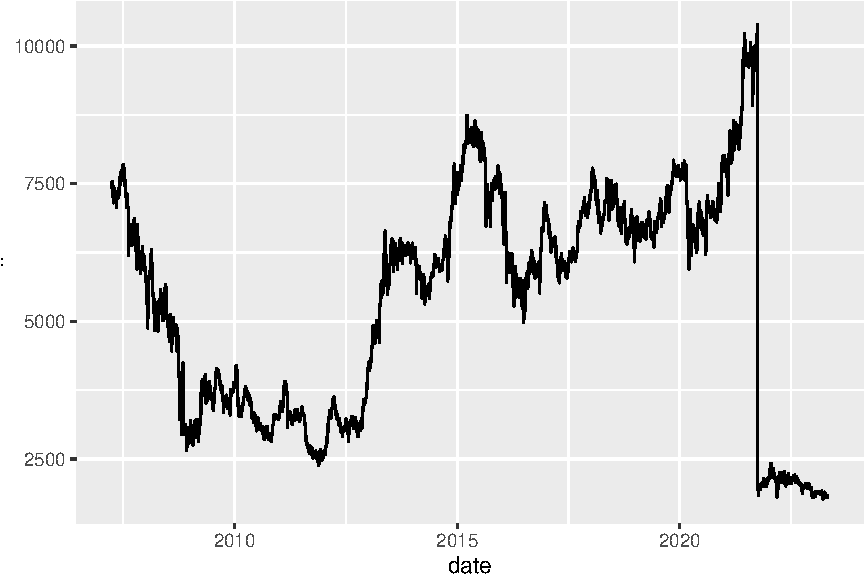
\includegraphics[keepaspectratio]{Hatakeda_Chap03_files/figure-pdf/unnamed-chunk-1-1.pdf}}

トヨタ自動車の2021年における株価の急落は,株式分割が原因です。
このとき,トヨタ自動車は1株を5株に分割しています。
そのため約10000円だった株価が約2000円と5分の1に下落したのです。

次にこのデータから株式リターンを計算し、折れ線グラフにしてみます。

\begin{Shaded}
\begin{Highlighting}[]
\NormalTok{df }\OtherTok{\textless{}{-}}\NormalTok{ df }\SpecialCharTok{\%\textgreater{}\%}
    \FunctionTok{group\_by}\NormalTok{(企業名) }\SpecialCharTok{\%\textgreater{}\%} \CommentTok{\# 企業名でグループ化}
    \FunctionTok{mutate}\NormalTok{(}
        \AttributeTok{r\_daily =}\NormalTok{ 終値 }\SpecialCharTok{/} \FunctionTok{lag}\NormalTok{(終値) }\SpecialCharTok{{-}}\DecValTok{1} \CommentTok{\# リターンを計算}
\NormalTok{    ) }\SpecialCharTok{\%\textgreater{}\%}
    \FunctionTok{filter}\NormalTok{(r\_daily }\SpecialCharTok{\textgreater{}} \SpecialCharTok{{-}}\FloatTok{0.5}\NormalTok{) }\CommentTok{\# 株式分割による異常値を除外}
\NormalTok{df }\SpecialCharTok{\%\textgreater{}\%}
    \FunctionTok{filter}\NormalTok{(企業名 }\SpecialCharTok{==} \StringTok{"トヨタ自動車"}\NormalTok{) }\SpecialCharTok{\%\textgreater{}\%} \CommentTok{\# トヨタ自動車を抽出}
    \FunctionTok{ggplot}\NormalTok{() }\SpecialCharTok{+} \FunctionTok{aes}\NormalTok{(}\AttributeTok{x =}\NormalTok{ date, }\AttributeTok{y =}\NormalTok{ r\_daily) }\SpecialCharTok{+} \FunctionTok{geom\_line}\NormalTok{() }\CommentTok{\# 折れ線グラフ}
\end{Highlighting}
\end{Shaded}

\pandocbounded{\includegraphics[keepaspectratio]{Hatakeda_Chap03_files/figure-pdf/unnamed-chunk-2-1.pdf}}

2021年の株式分割時の下落が異常な値となっていますが,それ以外の値動きは0を中心にランダムになっていることが分かります。

\section{期待値と分散(標準偏差)の推定}\label{ux671fux5f85ux5024ux3068ux5206ux6563ux6a19ux6e96ux504fux5deeux306eux63a8ux5b9a-1}

ある資産の価格やリターンを確率変数とみなしたとき,その背後にある\textbf{確率分布}の特徴を表す指標(つまり母数)を実際に観察することは不可能です。母集団のパラメータは観察不能なのです。
しかしながら,過去の観測値の集合である\textbf{データ}を用いて,確率分布の特徴やそれらの指標(期待値,分散,標準偏差)の\textbf{推定値}を求めることはできます。そこで,推定値を用いて確率変数の特徴を考察するようにします。

例えば,データから作成される\textbf{ヒストグラム}(histogram)や度数分布表は確率変数を特徴付ける確率分布の仮想となります。
期待値,分散,標準偏差の推定値は,確率変数を特徴付ける母平均(期待値),母分散,母標準偏差の仮想です。
この期待値,分散,標準偏差の推定値は,より具体的に\textbf{標本平均}(期待値),\textbf{標本分散},\textbf{標本標準偏差}とよばれます。
ただし「標本」という言葉はしばしば省略されることが多いので注意しましょう。

\begin{tcolorbox}[enhanced jigsaw, colframe=quarto-callout-important-color-frame, breakable, rightrule=.15mm, coltitle=black, title=\textcolor{quarto-callout-important-color}{\faExclamation}\hspace{0.5em}{(標本)単純平均}, colbacktitle=quarto-callout-important-color!10!white, leftrule=.75mm, colback=white, left=2mm, arc=.35mm, opacityback=0, titlerule=0mm, toptitle=1mm, bottomtitle=1mm, bottomrule=.15mm, toprule=.15mm, opacitybacktitle=0.6]

観測値\(x_k\)の単純平均値は, \[
\begin{aligned}
\bar X = \frac 1T \sum_{k=1}^T x_k
\end{aligned}
\] となる。
ここで\(T\)は観測値の数(これを\textbf{標本サイズ}という)を表します。

\end{tcolorbox}

\(t-1\)から\(t-T\)までの期間における資産\(i\)の標本期待(平均)リターン\(\bar r_i\)は,

\[
\begin{aligned}
\bar r_i = \frac 1T \sum _{k=1}^T r_{i,t-k}
\end{aligned}
\] となります。

\texttt{R}の基本関数だと\texttt{mean()}で計算できます。
たとえば,トヨタの株式リターンの平均は次の通りです。

\begin{Shaded}
\begin{Highlighting}[]
\FunctionTok{mean}\NormalTok{(df}\SpecialCharTok{$}\NormalTok{r\_daily[df}\SpecialCharTok{$}\NormalTok{企業名 }\SpecialCharTok{==} \StringTok{"トヨタ自動車"}\NormalTok{], }\AttributeTok{na.rm =} \ConstantTok{TRUE}\NormalTok{)}
\end{Highlighting}
\end{Shaded}

\begin{verbatim}
[1] 0.000225068
\end{verbatim}

このコードの意味するところは,\texttt{mean()}で引数のベクトルの平均を計算しています。
引数の\texttt{df\$r\_daily}とすることで,\texttt{df}というデータフレームの\texttt{r\_daily}という変数をしていしています。
さらに,\texttt{{[}df\$企業名\ ==\ "トヨタ自動車"{]}}と続けることで,\texttt{df}の\texttt{企業名}が\texttt{"トヨタ自動車"}となる行のみを抽出しています。
最後の\texttt{na.rm\ =\ TRUE}は,平均を出そうとするベクトルに欠損値が含まれている場合,その欠損値を除外して平均を計算することを意味しています。

計算されたトヨタ自動車の期待リターンは,\texttt{2.145399e-05}となりました。
これは指数表記で科学研究よく利用される書き方です。 数式で表現すると,

\[
2.145399 \times 10^{-5}
\]

のことで,具体的には,\(0.00002145399\)ということです。

標本(不偏)分散は,観測値\(x_k\)とその標本平均\(\bar X\)からの乖離の単純平均である。

\begin{tcolorbox}[enhanced jigsaw, colframe=quarto-callout-important-color-frame, breakable, rightrule=.15mm, coltitle=black, title=\textcolor{quarto-callout-important-color}{\faExclamation}\hspace{0.5em}{標本分散}, colbacktitle=quarto-callout-important-color!10!white, leftrule=.75mm, colback=white, left=2mm, arc=.35mm, opacityback=0, titlerule=0mm, toptitle=1mm, bottomtitle=1mm, bottomrule=.15mm, toprule=.15mm, opacitybacktitle=0.6]

\[
\begin{aligned}
s^2 [X] = \frac{1}{T-1} \sum _{k=1} (x_k - \bar X)^2
\end{aligned}
\]

\end{tcolorbox}

\(t-1\)から\(t-T\)までの期間における資産\(i\)のリターンの標本分散\(s^2[r_i]\)は,次の通りである。

\[
\begin{aligned}
s^2[r_i] = \frac{1}{T-1} \sum_{k=1}^T ( r_{i,t-k} - \bar r_i)^2
\end{aligned}
\]

\texttt{R}の基本関数だと\texttt{var()}で計算できます。
たとえば,トヨタの株式リターンの標本分散は次の通りです。

\begin{Shaded}
\begin{Highlighting}[]
\FunctionTok{var}\NormalTok{(df}\SpecialCharTok{$}\NormalTok{r\_daily[df}\SpecialCharTok{$}\NormalTok{企業名 }\SpecialCharTok{==} \StringTok{"トヨタ自動車"}\NormalTok{], }\AttributeTok{na.rm =} \ConstantTok{TRUE}\NormalTok{)}
\end{Highlighting}
\end{Shaded}

\begin{verbatim}
[1] 0.0003337524
\end{verbatim}

標本標準偏差は,分散の平方根です。

\begin{tcolorbox}[enhanced jigsaw, colframe=quarto-callout-important-color-frame, breakable, rightrule=.15mm, coltitle=black, title=\textcolor{quarto-callout-important-color}{\faExclamation}\hspace{0.5em}{標本標準偏差}, colbacktitle=quarto-callout-important-color!10!white, leftrule=.75mm, colback=white, left=2mm, arc=.35mm, opacityback=0, titlerule=0mm, toptitle=1mm, bottomtitle=1mm, bottomrule=.15mm, toprule=.15mm, opacitybacktitle=0.6]

\[
\begin{aligned}
s [X] = \sqrt{s^2[X]}
\end{aligned}
\]

\end{tcolorbox}

\(t-1\)から\(t-T\)までの期間における資産\(i\)のリターンの標本標準偏差\(s[r_i]\)は,次の通りである。

\[
\begin{aligned}
s [r_i] = \sqrt{s^2 [r_i]}
\end{aligned}
\]

\texttt{R}の基本関数で標準偏差を返す関数は\texttt{sd()}です。
たとえば,トヨタの株式リターンの標本標準偏差は次の通りです。

\begin{Shaded}
\begin{Highlighting}[]
\FunctionTok{sd}\NormalTok{(df}\SpecialCharTok{$}\NormalTok{r\_daily[df}\SpecialCharTok{$}\NormalTok{企業名 }\SpecialCharTok{==} \StringTok{"トヨタ自動車"}\NormalTok{], }\AttributeTok{na.rm =} \ConstantTok{TRUE}\NormalTok{)}
\end{Highlighting}
\end{Shaded}

\begin{verbatim}
[1] 0.01826889
\end{verbatim}

データから確率分布の特性を表す指標にはほかにも色々あります。
たとえば尖度や歪度などです。尖度(skewness)とは,確率分布の尖り具合を表す指標です。
歪度(kurtosis)とは,確率分布の裾の重さを表す指標です。

多様な統計量から分布の特徴を捉えることも重要ですが、グラフの1つである\textbf{ヒストグラム}(histogram)は数値よりも直観的に分布の形を確認できるため,まず度数分布表やヒストグラムを作成することをお勧めします。
\texttt{R}の基本関数でヒストグラムを作成するには\texttt{hist()}を用います。
いままでと同様に、トヨタ自動車の株式リターンのヒストグラムを作成してみましょう。

\begin{Shaded}
\begin{Highlighting}[]
\CommentTok{\# par(family = "HiraKakuProN{-}W3") \# macの文字化け対策 winの人はコメントアウト}
\FunctionTok{hist}\NormalTok{(df}\SpecialCharTok{$}\NormalTok{r\_daily[df}\SpecialCharTok{$}\NormalTok{企業名 }\SpecialCharTok{==} \StringTok{"トヨタ自動車"}\NormalTok{]) }\CommentTok{\# 基本関数でヒストグラム}
\end{Highlighting}
\end{Shaded}

\pandocbounded{\includegraphics[keepaspectratio]{Hatakeda_Chap03_files/figure-pdf/unnamed-chunk-6-1.pdf}}

これでももちろんヒストグラムを作成することはできるのですが、
よりキレイなグラフを作成したいなら、\texttt{tidyverse}の\texttt{ggplot2}パッケージが便利です。
ただし,\texttt{ggplot2}で利用できるデータの型は\texttt{data.frame}型に限るので注意しましょう。

まず、作図のためのデータを用意します。
トヨタ自動車の日次リターンと日付を抽出し、\texttt{data.frame}型に変換して,\texttt{df\_toyota}という変数に格納します。

\begin{Shaded}
\begin{Highlighting}[]
\NormalTok{df\_toyota }\OtherTok{\textless{}{-}}\NormalTok{ df }\SpecialCharTok{\%\textgreater{}\%}
    \FunctionTok{filter}\NormalTok{(企業名 }\SpecialCharTok{==} \StringTok{"トヨタ自動車"}\NormalTok{) }\SpecialCharTok{\%\textgreater{}\%}
    \FunctionTok{select}\NormalTok{(date, r\_daily)}
\end{Highlighting}
\end{Shaded}

つぎに,\texttt{ggplot()}関数で作図してみます。
ggplot2パッケージでは,以下の要素を指定してグラフを作ります。

\begin{itemize}
\tightlist
\item
  \texttt{ggplot()}関数でデータを指定
\item
  \texttt{aes()}関数でx軸とy軸の変数を指定
\item
  \texttt{geom\_***}関数でグラフの種類を指定
\end{itemize}

たとえば,\texttt{geom\_histogram()}関数を用いるとヒストグラムを作成できます。

\begin{Shaded}
\begin{Highlighting}[]
\NormalTok{g }\OtherTok{\textless{}{-}} \FunctionTok{ggplot}\NormalTok{(df\_toyota) }\SpecialCharTok{+} \CommentTok{\# データを指定}
    \FunctionTok{aes}\NormalTok{(}\AttributeTok{x =}\NormalTok{ r\_daily) }\SpecialCharTok{+}  \CommentTok{\# 変数を指定}
    \FunctionTok{geom\_histogram}\NormalTok{() }\CommentTok{\# グラフを指定}
\NormalTok{g }\OtherTok{\textless{}{-}}\NormalTok{ g }\SpecialCharTok{+} \FunctionTok{xlim}\NormalTok{(}\SpecialCharTok{{-}}\FloatTok{0.1}\NormalTok{, }\FloatTok{0.1}\NormalTok{) }\CommentTok{\# x軸の範囲を指定}
\NormalTok{g }\OtherTok{\textless{}{-}}\NormalTok{ g }\SpecialCharTok{+} \FunctionTok{xlab}\NormalTok{(}\StringTok{"日次リターン"}\NormalTok{) }\SpecialCharTok{+} \FunctionTok{ylab}\NormalTok{(}\StringTok{"度数"}\NormalTok{) }\CommentTok{\# x軸とy軸のラベルを指定}
\FunctionTok{print}\NormalTok{(g) }\CommentTok{\# 出力}
\end{Highlighting}
\end{Shaded}

\pandocbounded{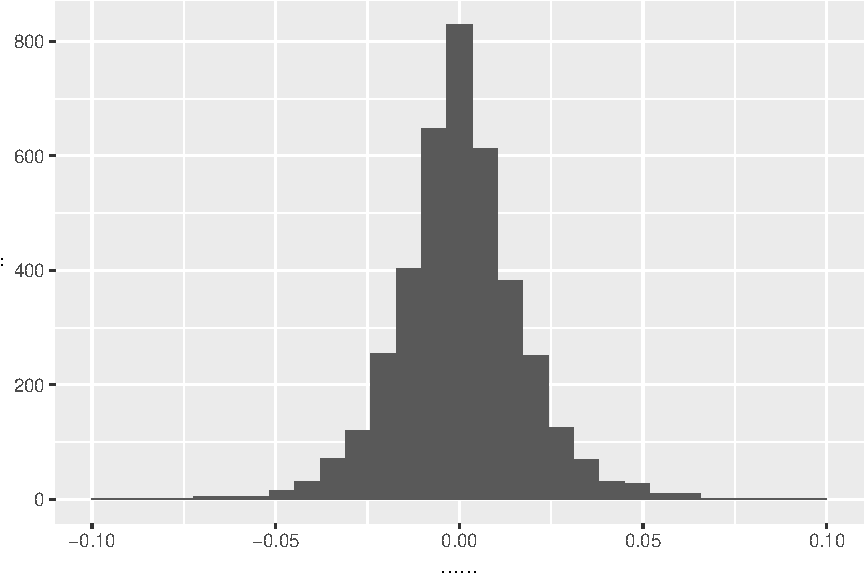
\includegraphics[keepaspectratio]{Hatakeda_Chap03_files/figure-pdf/unnamed-chunk-8-1.pdf}}

正規分布のように左右対称の分布になっていることが分かります。

ここまでの学習から,1変数の離散確率変数の特徴を表す指標として,期待値,分散,標準偏差を学習し,またデータの分布を視覚的に把握するグラフとしてヒストグラムの作り方を学習しました。
それぞれの定義,計算方法,作図方法を理解し,説明できるようになっていれば,この節は終了です。
次節から,2変数間の関係を表す統計量について学習します。

\section{共分散と相関係数の推定}\label{ux5171ux5206ux6563ux3068ux76f8ux95a2ux4fc2ux6570ux306eux63a8ux5b9a}

2つの確率変数間の特徴を表す指標として、\textbf{共分散}(covariance)と\textbf{相関係数}(correlation
coefficient)を学習します。
いま,観察される確率変数\(X\)と\(Z\)の実現値の組\((x_i, z_i), i = 1, \dots , N\)がデータとして手元にあるとします。
ここで,\(N\)は標本サイズを表しています。つまり\(N\)個のデータの組があるということです。
この\(N\)個のデータを座標平面上で表したものを\textbf{散布図}(scatter
diagram)といいます。
たとえば、トヨタ自動車と日産自動車の株式リターンの散布図を作成してみましょう。

\begin{Shaded}
\begin{Highlighting}[]
\NormalTok{df }\SpecialCharTok{\%\textgreater{}\%}
    \FunctionTok{filter}\NormalTok{(企業名 }\SpecialCharTok{==} \StringTok{"トヨタ自動車"} \SpecialCharTok{|}\NormalTok{ 企業名 }\SpecialCharTok{==} \StringTok{"日産自動車"}\NormalTok{) }\SpecialCharTok{\%\textgreater{}\%}
    \FunctionTok{select}\NormalTok{(企業名, date, r\_daily) }\SpecialCharTok{\%\textgreater{}\%}
    \FunctionTok{pivot\_wider}\NormalTok{(}\AttributeTok{names\_from =}\NormalTok{ 企業名, }\AttributeTok{values\_from =}\NormalTok{ r\_daily) }\SpecialCharTok{\%\textgreater{}\%}
    \FunctionTok{ggplot}\NormalTok{() }\SpecialCharTok{+} \FunctionTok{aes}\NormalTok{(}\AttributeTok{x =}\NormalTok{ トヨタ自動車, }\AttributeTok{y =}\NormalTok{ 日産自動車) }\SpecialCharTok{+} \FunctionTok{geom\_point}\NormalTok{()}
\end{Highlighting}
\end{Shaded}

\pandocbounded{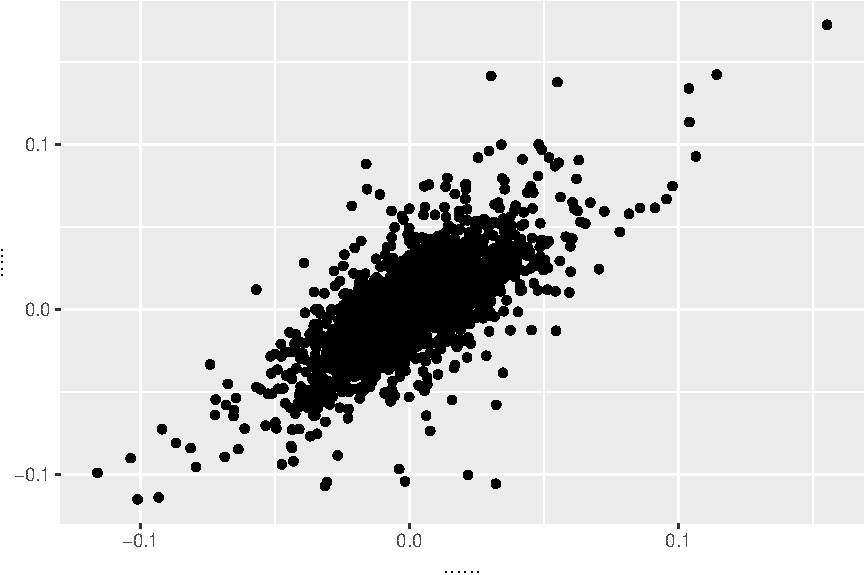
\includegraphics[keepaspectratio]{Hatakeda_Chap03_files/figure-pdf/unnamed-chunk-9-1.pdf}}

この散布図から,トヨタ自動車と日産自動車の株式リターンはどちらかの株式リターンが増加したら,もう片方も増加する,という関係にあるといえます。
この関係の強さを数値で表したものが共分散や相関係数となります。
共分散は,次のように定義される。

\begin{tcolorbox}[enhanced jigsaw, colframe=quarto-callout-important-color-frame, breakable, rightrule=.15mm, coltitle=black, title=\textcolor{quarto-callout-important-color}{\faExclamation}\hspace{0.5em}{共分散}, colbacktitle=quarto-callout-important-color!10!white, leftrule=.75mm, colback=white, left=2mm, arc=.35mm, opacityback=0, titlerule=0mm, toptitle=1mm, bottomtitle=1mm, bottomrule=.15mm, toprule=.15mm, opacitybacktitle=0.6]

共分散の定義は,

\[
\begin{aligned}
s_{XZ} = \frac{1}{N} \sum_{i=1}^N (x_i - \bar X)(z_i - \bar Z)
\end{aligned}
\]

\end{tcolorbox}

共分散は,\(X\)と\(Z\)の標本平均からの乖離の単純平均となります。
図で示すと,次のようになります。

\begin{Shaded}
\begin{Highlighting}[]
\NormalTok{df }\SpecialCharTok{\%\textgreater{}\%}
    \FunctionTok{filter}\NormalTok{(企業名 }\SpecialCharTok{==} \StringTok{"トヨタ自動車"} \SpecialCharTok{|}\NormalTok{ 企業名 }\SpecialCharTok{==} \StringTok{"日産自動車"}\NormalTok{) }\SpecialCharTok{\%\textgreater{}\%}
    \FunctionTok{select}\NormalTok{(企業名, date, r\_daily) }\SpecialCharTok{\%\textgreater{}\%}
    \FunctionTok{pivot\_wider}\NormalTok{(}\AttributeTok{names\_from =}\NormalTok{ 企業名, }\AttributeTok{values\_from =}\NormalTok{ r\_daily) }\SpecialCharTok{\%\textgreater{}\%}
    \FunctionTok{ggplot}\NormalTok{() }\SpecialCharTok{+} \FunctionTok{aes}\NormalTok{(}\AttributeTok{x =}\NormalTok{ トヨタ自動車, }\AttributeTok{y =}\NormalTok{ 日産自動車) }\SpecialCharTok{+} \FunctionTok{geom\_point}\NormalTok{() }\SpecialCharTok{+}
    \FunctionTok{geom\_vline}\NormalTok{(}\AttributeTok{xintercept =} \FunctionTok{mean}\NormalTok{(df}\SpecialCharTok{$}\NormalTok{r\_daily[df}\SpecialCharTok{$}\NormalTok{企業名 }\SpecialCharTok{==} \StringTok{"トヨタ自動車"}\NormalTok{], }\AttributeTok{na.rm =} \ConstantTok{TRUE}\NormalTok{), }\AttributeTok{linetype =} \StringTok{"dashed"}\NormalTok{,}\AttributeTok{color =} \StringTok{"red"}\NormalTok{) }\SpecialCharTok{+}
    \FunctionTok{geom\_hline}\NormalTok{(}\AttributeTok{yintercept =} \FunctionTok{mean}\NormalTok{(df}\SpecialCharTok{$}\NormalTok{r\_daily[df}\SpecialCharTok{$}\NormalTok{企業名 }\SpecialCharTok{==} \StringTok{"日産自動車"}\NormalTok{], }\AttributeTok{na.rm =} \ConstantTok{TRUE}\NormalTok{), }\AttributeTok{linetype =} \StringTok{"dashed"}\NormalTok{, }\AttributeTok{color =} \StringTok{"red"}\NormalTok{)}
\end{Highlighting}
\end{Shaded}

\pandocbounded{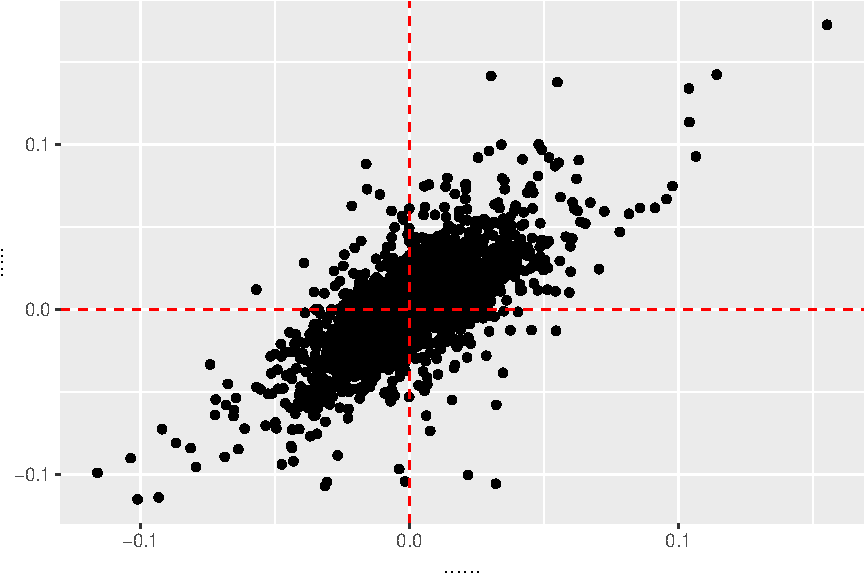
\includegraphics[keepaspectratio]{Hatakeda_Chap03_files/figure-pdf/unnamed-chunk-10-1.pdf}}

この第1象限(右上)に位置する実現値の組\((x_i, z_i)\)は,\(x_i > \bar X\)かつ\(z_i > \bar Z\)であり,また第3象限(左下)の領域の点も\(x_i < \bar X\)かつ\(z_i < \bar Z\)であるため,\((x_i - \bar X)(z_i - \bar Z)\)は正の値をとります。
つまり,第1象限と第3象限の点の組み合わせが多いとき,共分散の値を正にする方向に寄与し,第2象限と第4象限は負に寄与します。
よってトヨタ自動車と日産自動車の株式リターンの共分散は正になることが予想されます。
では計算してみましょう。

\begin{Shaded}
\begin{Highlighting}[]
\NormalTok{df\_cov }\OtherTok{\textless{}{-}}\NormalTok{ df }\SpecialCharTok{\%\textgreater{}\%}
    \FunctionTok{filter}\NormalTok{(企業名 }\SpecialCharTok{==} \StringTok{"トヨタ自動車"} \SpecialCharTok{|}\NormalTok{ 企業名 }\SpecialCharTok{==} \StringTok{"日産自動車"}\NormalTok{) }\SpecialCharTok{\%\textgreater{}\%}
    \FunctionTok{select}\NormalTok{(企業名, date, r\_daily) }\SpecialCharTok{\%\textgreater{}\%} \CommentTok{\# 変数を選択}
    \FunctionTok{pivot\_wider}\NormalTok{(}\AttributeTok{names\_from =}\NormalTok{ 企業名, }\AttributeTok{values\_from =}\NormalTok{ r\_daily) }\SpecialCharTok{\%\textgreater{}\%} \CommentTok{\# 横データに}
    \FunctionTok{drop\_na}\NormalTok{() }\CommentTok{\# 欠損値を削除}
\NormalTok{(cov\_toyota\_nissan }\OtherTok{\textless{}{-}} \FunctionTok{cov}\NormalTok{(df\_cov}\SpecialCharTok{$}\NormalTok{トヨタ自動車, df\_cov}\SpecialCharTok{$}\NormalTok{日産自動車))}
\end{Highlighting}
\end{Shaded}

\begin{verbatim}
[1] 0.0003021892
\end{verbatim}

トヨタ自動車と日産自動車の株式リターンの共分散は\ensuremath{3\times 10^{-4}}となり,正の値であることが分かりました。
共分散は2変数間の関係をします尺度ですが、その値の大きさは単位に依存するという問題があります。
そこで、共分散を標準化したものが相関係数です。
相関係数は、共分散を各変数の標準偏差で割ったものです。

\begin{tcolorbox}[enhanced jigsaw, colframe=quarto-callout-important-color-frame, breakable, rightrule=.15mm, coltitle=black, title=\textcolor{quarto-callout-important-color}{\faExclamation}\hspace{0.5em}{相関係数}, colbacktitle=quarto-callout-important-color!10!white, leftrule=.75mm, colback=white, left=2mm, arc=.35mm, opacityback=0, titlerule=0mm, toptitle=1mm, bottomtitle=1mm, bottomrule=.15mm, toprule=.15mm, opacitybacktitle=0.6]

相関係数の定義は,

\[
\begin{aligned}
\rho_{XZ} = \frac{\mathbb{COV}[XZ]}{s[X] \times  s[Z]}
\end{aligned}
\]

\end{tcolorbox}

相関係数は変数の単位に依存せず、\(-1 \leq \rho_{XZ} \leq 1\)の値をとる尺度で、2変数間の関係の強さを表します。
相関係数が\(1\)に近いほど正の相関が強く、\(-1\)に近いほど負の相関が強いといえます。
また、相関係数が\(0\)に近いほど2変数間の関係は弱いといえます。

標本相関係数\(\rho _{XZ}\)が\(0.5\)の場合、以下のような散布図になります。

\begin{Shaded}
\begin{Highlighting}[]
\NormalTok{X }\OtherTok{\textless{}{-}} \FunctionTok{rnorm}\NormalTok{(}\DecValTok{1000}\NormalTok{, }\AttributeTok{mean =} \DecValTok{0}\NormalTok{, }\AttributeTok{sd =} \DecValTok{1}\NormalTok{)}
\NormalTok{Z }\OtherTok{\textless{}{-}} \FloatTok{0.5} \SpecialCharTok{*}\NormalTok{ X }\SpecialCharTok{+} \FunctionTok{rnorm}\NormalTok{(}\DecValTok{1000}\NormalTok{, }\AttributeTok{mean =} \DecValTok{0}\NormalTok{, }\AttributeTok{sd =} \DecValTok{1}\NormalTok{)}
\NormalTok{df }\OtherTok{\textless{}{-}} \FunctionTok{data.frame}\NormalTok{(X, Z)}
\FunctionTok{ggplot}\NormalTok{(df) }\SpecialCharTok{+} \FunctionTok{aes}\NormalTok{(}\AttributeTok{x =}\NormalTok{ X, }\AttributeTok{y =}\NormalTok{ Z) }\SpecialCharTok{+} \FunctionTok{geom\_point}\NormalTok{()}
\end{Highlighting}
\end{Shaded}

\pandocbounded{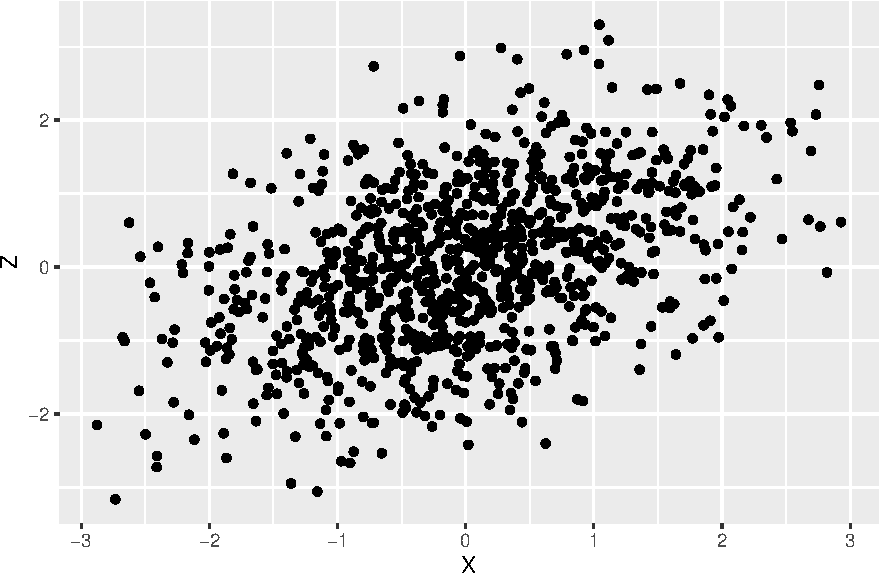
\includegraphics[keepaspectratio]{Hatakeda_Chap03_files/figure-pdf/unnamed-chunk-12-1.pdf}}

標本相関係数\(\rho _{XZ}\)が\(0.90\)の場合、以下のような散布図になります。

\begin{Shaded}
\begin{Highlighting}[]
\NormalTok{X }\OtherTok{\textless{}{-}} \FunctionTok{rnorm}\NormalTok{(}\DecValTok{1000}\NormalTok{, }\AttributeTok{mean =} \DecValTok{0}\NormalTok{, }\AttributeTok{sd =} \DecValTok{1}\NormalTok{)}
\NormalTok{Z }\OtherTok{\textless{}{-}} \FloatTok{0.9} \SpecialCharTok{*}\NormalTok{ X }\SpecialCharTok{+} \FunctionTok{rnorm}\NormalTok{(}\DecValTok{1000}\NormalTok{, }\AttributeTok{mean =} \DecValTok{0}\NormalTok{, }\AttributeTok{sd =} \DecValTok{1}\NormalTok{)}
\NormalTok{df }\OtherTok{\textless{}{-}} \FunctionTok{data.frame}\NormalTok{(X, Z)}
\FunctionTok{ggplot}\NormalTok{(df) }\SpecialCharTok{+} \FunctionTok{aes}\NormalTok{(}\AttributeTok{x =}\NormalTok{ X, }\AttributeTok{y =}\NormalTok{ Z) }\SpecialCharTok{+} \FunctionTok{geom\_point}\NormalTok{()}
\end{Highlighting}
\end{Shaded}

\pandocbounded{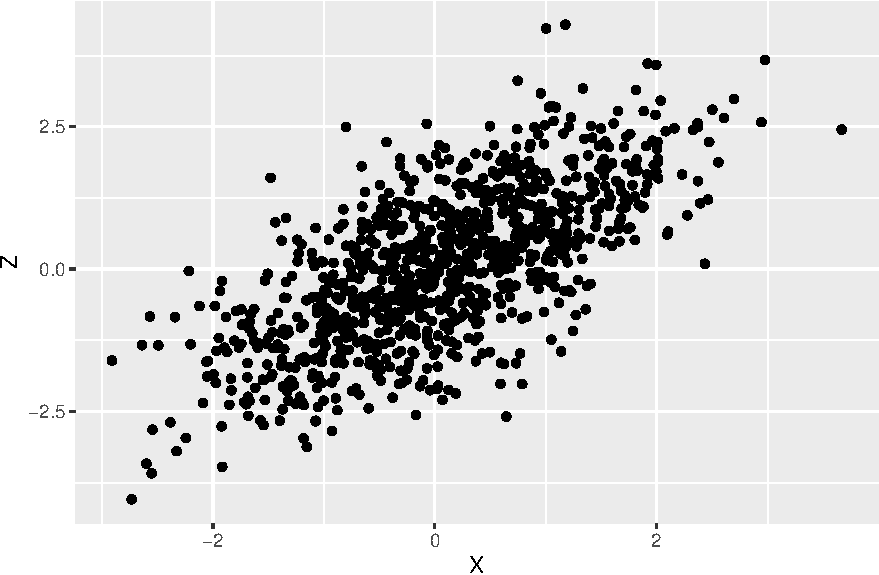
\includegraphics[keepaspectratio]{Hatakeda_Chap03_files/figure-pdf/unnamed-chunk-13-1.pdf}}

標本相関係数\(\rho _{XZ}\)が\(-0.6\)の場合、以下のような散布図になります。

\begin{Shaded}
\begin{Highlighting}[]
\NormalTok{X }\OtherTok{\textless{}{-}} \FunctionTok{rnorm}\NormalTok{(}\DecValTok{1000}\NormalTok{, }\AttributeTok{mean =} \DecValTok{0}\NormalTok{, }\AttributeTok{sd =} \DecValTok{1}\NormalTok{)}
\NormalTok{Z }\OtherTok{\textless{}{-}} \SpecialCharTok{{-}}\FloatTok{0.6} \SpecialCharTok{*}\NormalTok{ X }\SpecialCharTok{+} \FunctionTok{rnorm}\NormalTok{(}\DecValTok{1000}\NormalTok{, }\AttributeTok{mean =} \DecValTok{0}\NormalTok{, }\AttributeTok{sd =} \DecValTok{1}\NormalTok{)}
\NormalTok{df }\OtherTok{\textless{}{-}} \FunctionTok{data.frame}\NormalTok{(X, Z)}
\FunctionTok{ggplot}\NormalTok{(df) }\SpecialCharTok{+} \FunctionTok{aes}\NormalTok{(}\AttributeTok{x =}\NormalTok{ X, }\AttributeTok{y =}\NormalTok{ Z) }\SpecialCharTok{+} \FunctionTok{geom\_point}\NormalTok{()}
\end{Highlighting}
\end{Shaded}

\pandocbounded{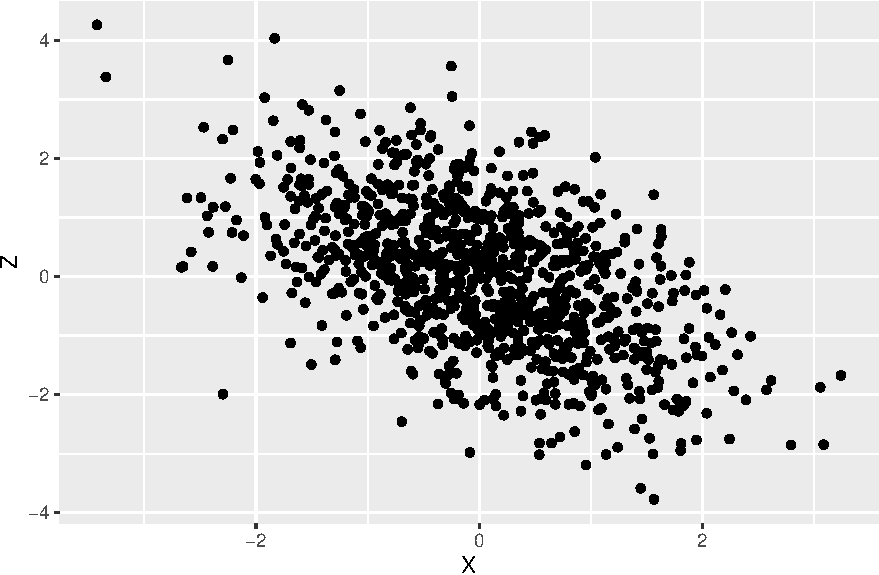
\includegraphics[keepaspectratio]{Hatakeda_Chap03_files/figure-pdf/unnamed-chunk-14-1.pdf}}

無相関,つまり標本相関係数\(\rho _{XZ}\)が\(0\)の場合、以下のような散布図になります。

\begin{Shaded}
\begin{Highlighting}[]
\NormalTok{X }\OtherTok{\textless{}{-}} \FunctionTok{rnorm}\NormalTok{(}\DecValTok{1000}\NormalTok{, }\AttributeTok{mean =} \DecValTok{0}\NormalTok{, }\AttributeTok{sd =} \DecValTok{1}\NormalTok{)}
\NormalTok{Z }\OtherTok{\textless{}{-}} \FunctionTok{rnorm}\NormalTok{(}\DecValTok{1000}\NormalTok{, }\AttributeTok{mean =} \DecValTok{0}\NormalTok{, }\AttributeTok{sd =} \DecValTok{1}\NormalTok{)}
\NormalTok{df }\OtherTok{\textless{}{-}} \FunctionTok{data.frame}\NormalTok{(X, Z)}
\FunctionTok{ggplot}\NormalTok{(df) }\SpecialCharTok{+} \FunctionTok{aes}\NormalTok{(}\AttributeTok{x =}\NormalTok{ X, }\AttributeTok{y =}\NormalTok{ Z) }\SpecialCharTok{+} \FunctionTok{geom\_point}\NormalTok{()}
\end{Highlighting}
\end{Shaded}

\pandocbounded{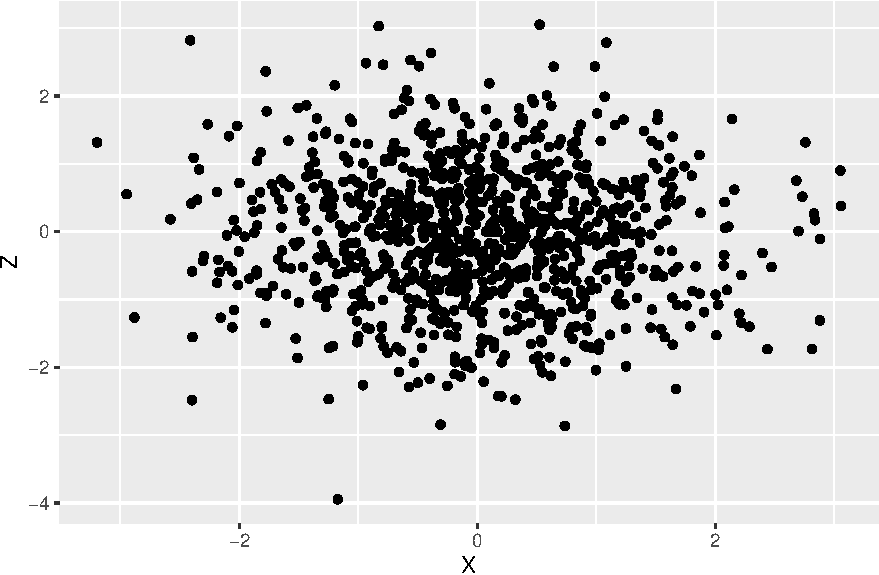
\includegraphics[keepaspectratio]{Hatakeda_Chap03_files/figure-pdf/unnamed-chunk-15-1.pdf}}

注意しないといけないのは,相関係数が線形関係を前提とした尺度であることです。もし2変数の関係が非線形である場合は,相関係数は役に立ちません。
たとえば,いかのような有名な図があります。

\begin{Shaded}
\begin{Highlighting}[]
\FunctionTok{ggplot}\NormalTok{(datasaurus\_dozen) }\SpecialCharTok{+} \FunctionTok{aes}\NormalTok{(}\AttributeTok{x =}\NormalTok{ x, }\AttributeTok{y =}\NormalTok{ y, }\AttributeTok{color =}\NormalTok{ dataset) }\SpecialCharTok{+} \FunctionTok{geom\_point}\NormalTok{() }\SpecialCharTok{+} \FunctionTok{facet\_wrap}\NormalTok{(}\SpecialCharTok{\textasciitilde{}}\NormalTok{dataset, }\AttributeTok{ncol =} \DecValTok{3}\NormalTok{) }\SpecialCharTok{+} \FunctionTok{theme\_bw}\NormalTok{() }\SpecialCharTok{+} \FunctionTok{theme}\NormalTok{(}\AttributeTok{panel.grid =} \FunctionTok{element\_blank}\NormalTok{())}
\end{Highlighting}
\end{Shaded}

\pandocbounded{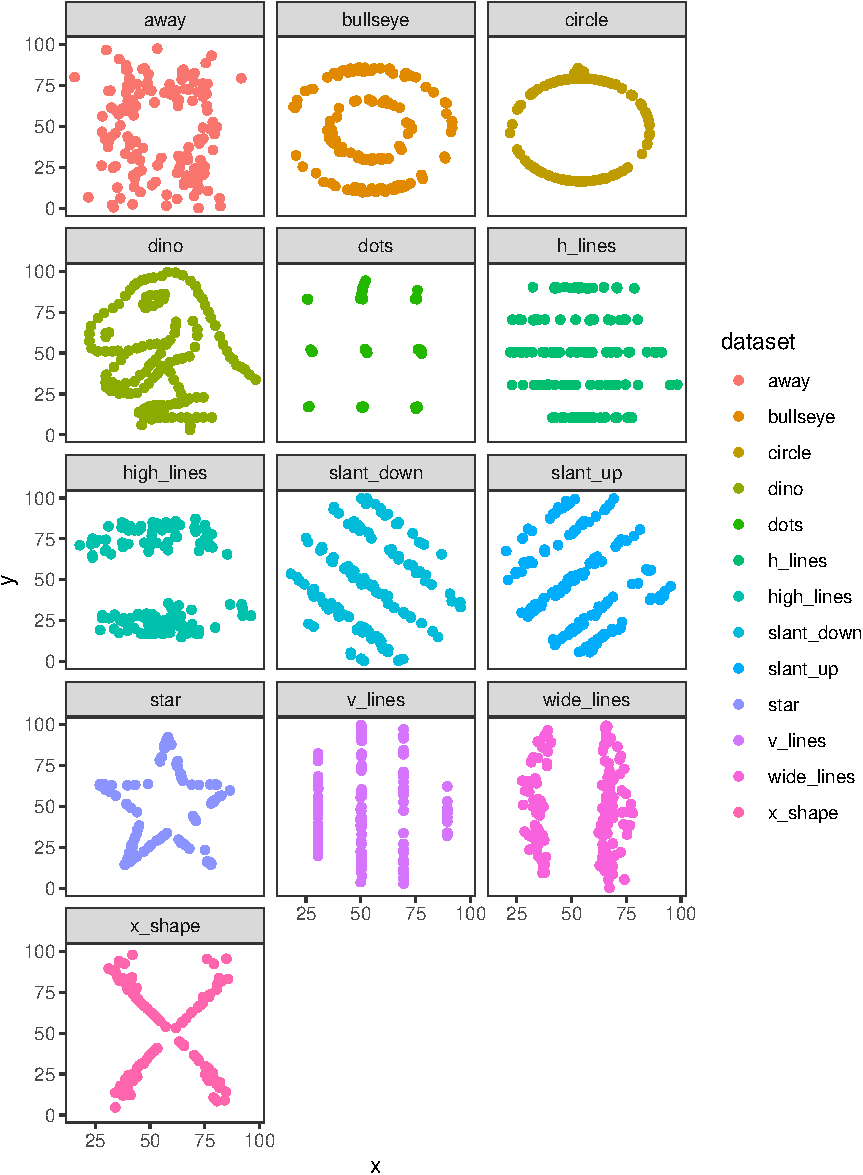
\includegraphics[keepaspectratio]{Hatakeda_Chap03_files/figure-pdf/unnamed-chunk-16-1.pdf}}

アニメーションにするとこうなります。
\texttt{gganimate}パッケージの\texttt{transition\_states()}関数を用いてアニメーションを作成しています。

\begin{Shaded}
\begin{Highlighting}[]
\FunctionTok{ggplot}\NormalTok{(datasaurus\_dozen, }\FunctionTok{aes}\NormalTok{(}\AttributeTok{x =}\NormalTok{ x, }\AttributeTok{y =}\NormalTok{ y))}\SpecialCharTok{+}
  \FunctionTok{geom\_point}\NormalTok{() }\SpecialCharTok{+} \FunctionTok{theme\_minimal}\NormalTok{() }\SpecialCharTok{+}
  \FunctionTok{transition\_states}\NormalTok{(dataset, }\DecValTok{3}\NormalTok{, }\DecValTok{1}\NormalTok{)}
\end{Highlighting}
\end{Shaded}

\pandocbounded{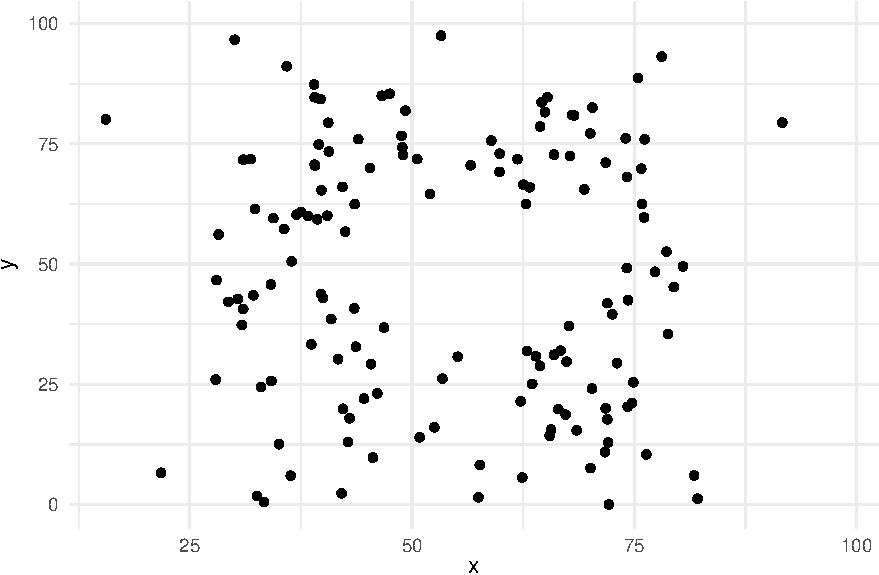
\includegraphics[keepaspectratio]{Hatakeda_Chap03_files/figure-pdf/unnamed-chunk-17-1.pdf}}

\pandocbounded{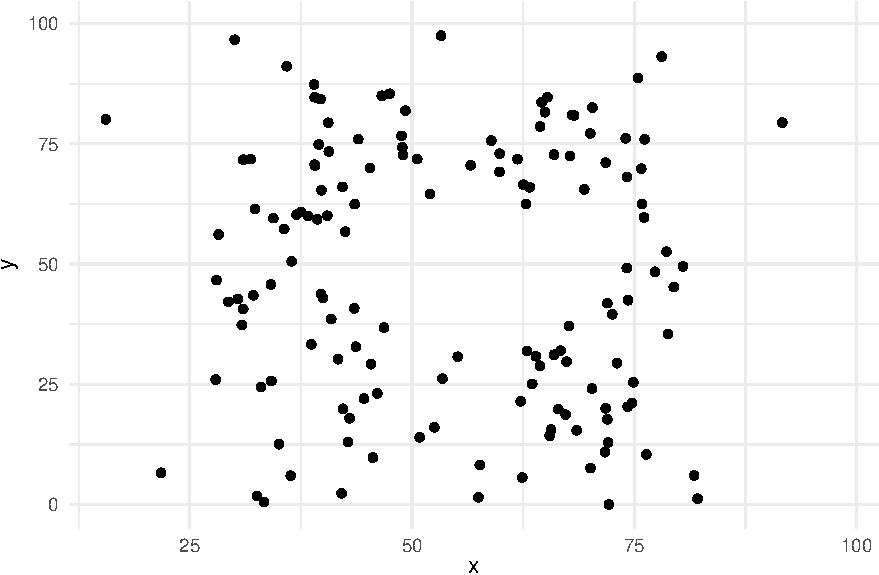
\includegraphics[keepaspectratio]{Hatakeda_Chap03_files/figure-pdf/unnamed-chunk-17-2.pdf}}

\pandocbounded{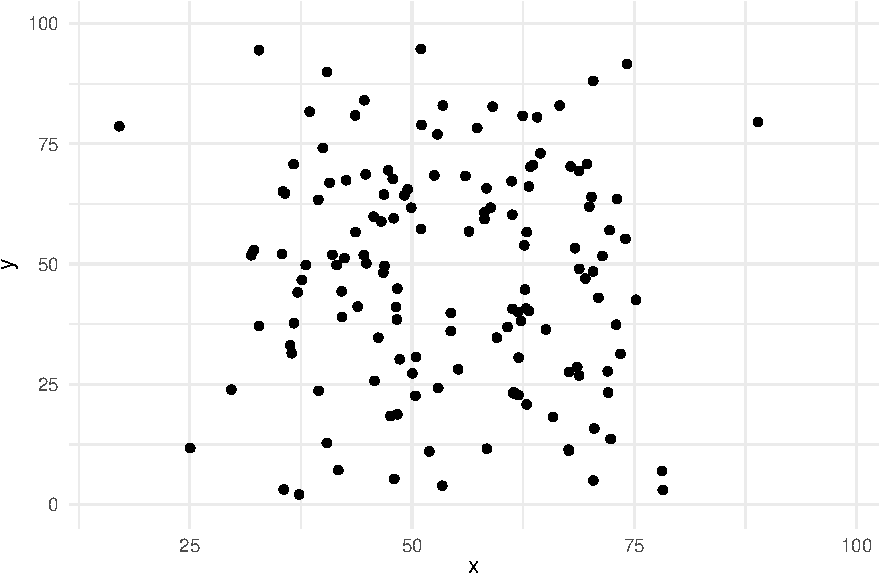
\includegraphics[keepaspectratio]{Hatakeda_Chap03_files/figure-pdf/unnamed-chunk-17-3.pdf}}

\pandocbounded{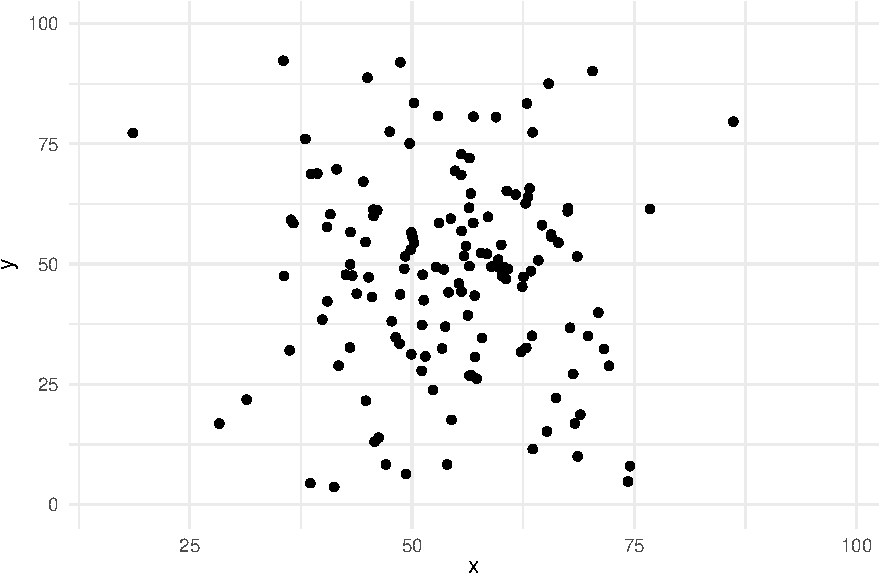
\includegraphics[keepaspectratio]{Hatakeda_Chap03_files/figure-pdf/unnamed-chunk-17-4.pdf}}

\pandocbounded{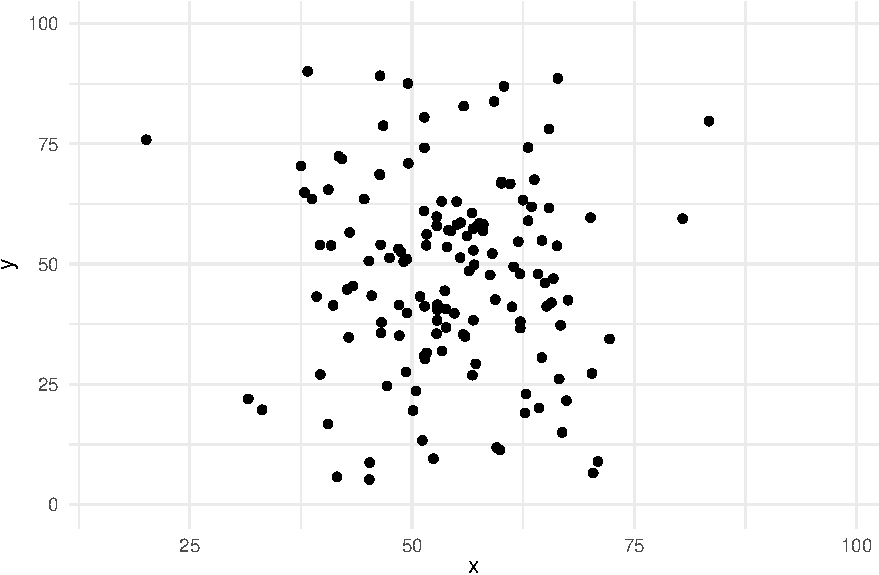
\includegraphics[keepaspectratio]{Hatakeda_Chap03_files/figure-pdf/unnamed-chunk-17-5.pdf}}

\pandocbounded{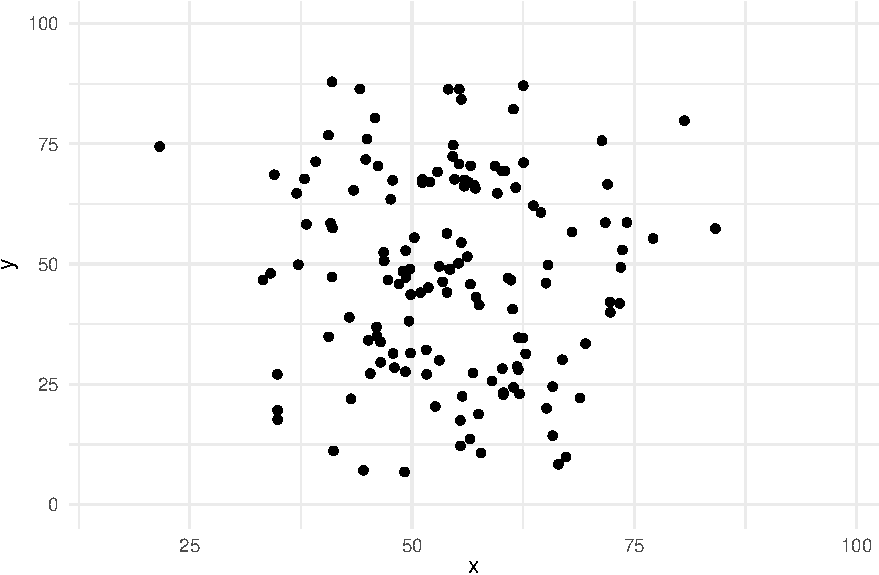
\includegraphics[keepaspectratio]{Hatakeda_Chap03_files/figure-pdf/unnamed-chunk-17-6.pdf}}

\pandocbounded{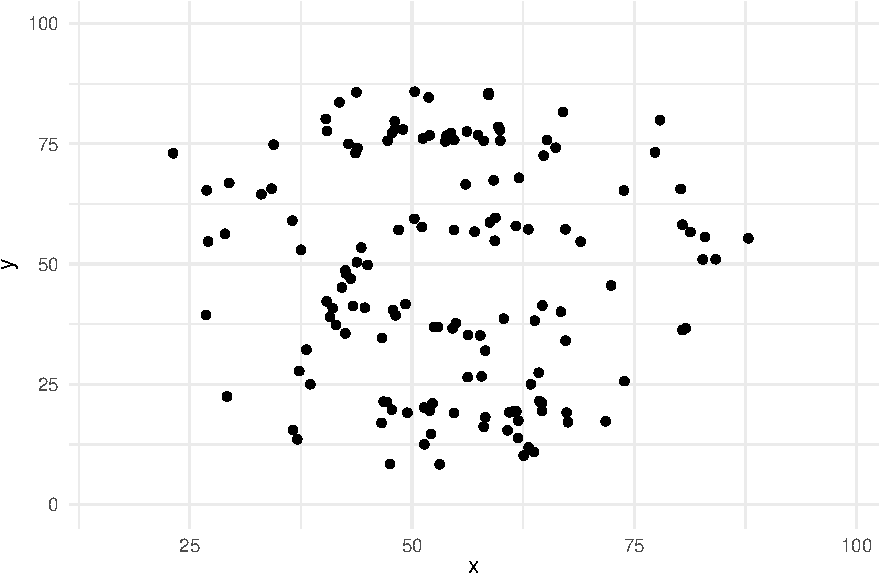
\includegraphics[keepaspectratio]{Hatakeda_Chap03_files/figure-pdf/unnamed-chunk-17-7.pdf}}

\pandocbounded{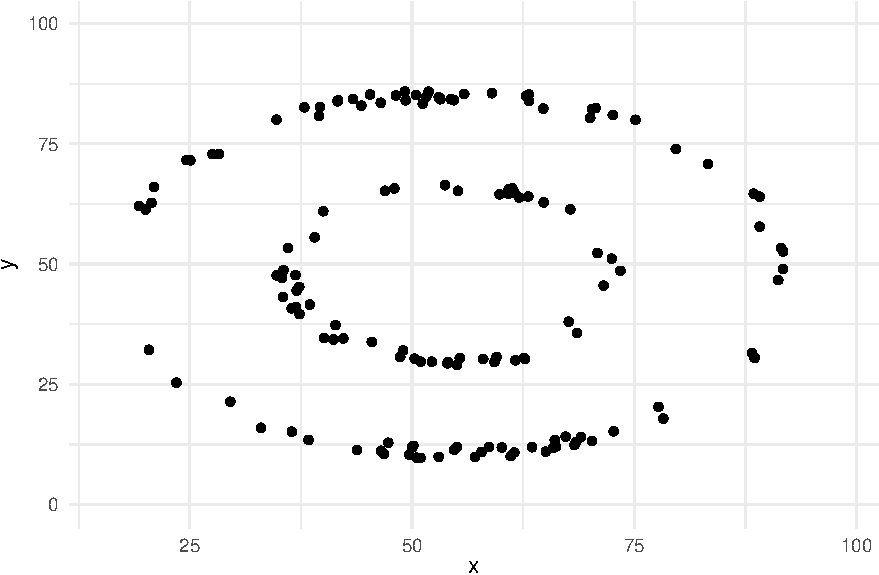
\includegraphics[keepaspectratio]{Hatakeda_Chap03_files/figure-pdf/unnamed-chunk-17-8.pdf}}

\pandocbounded{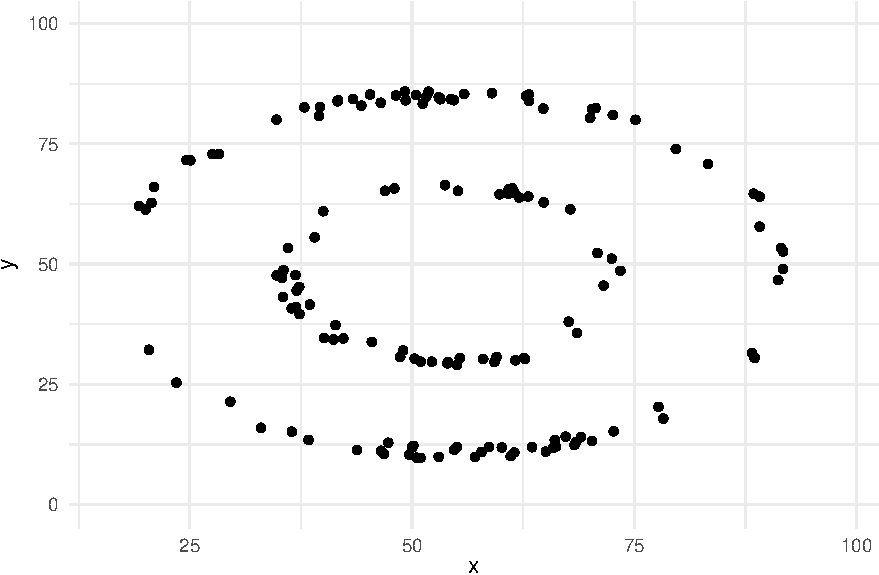
\includegraphics[keepaspectratio]{Hatakeda_Chap03_files/figure-pdf/unnamed-chunk-17-9.pdf}}

\pandocbounded{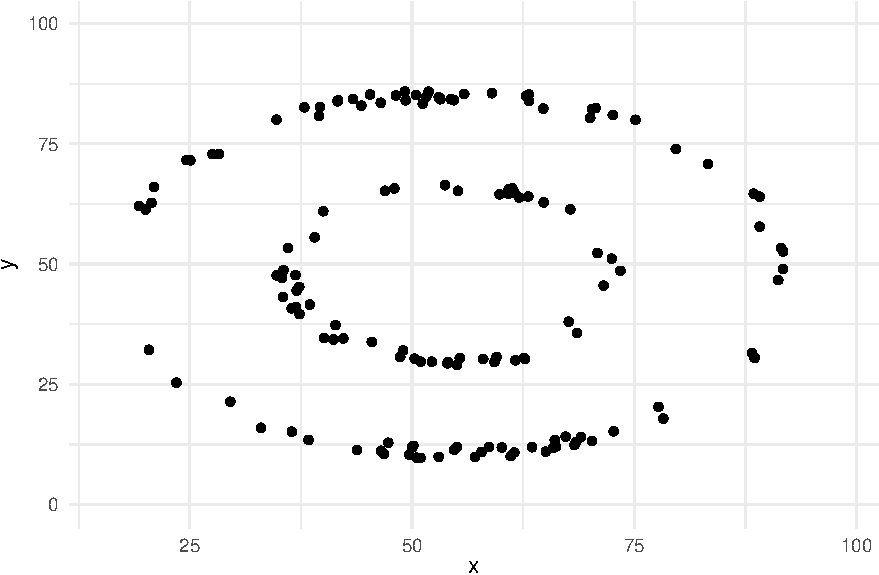
\includegraphics[keepaspectratio]{Hatakeda_Chap03_files/figure-pdf/unnamed-chunk-17-10.pdf}}

\pandocbounded{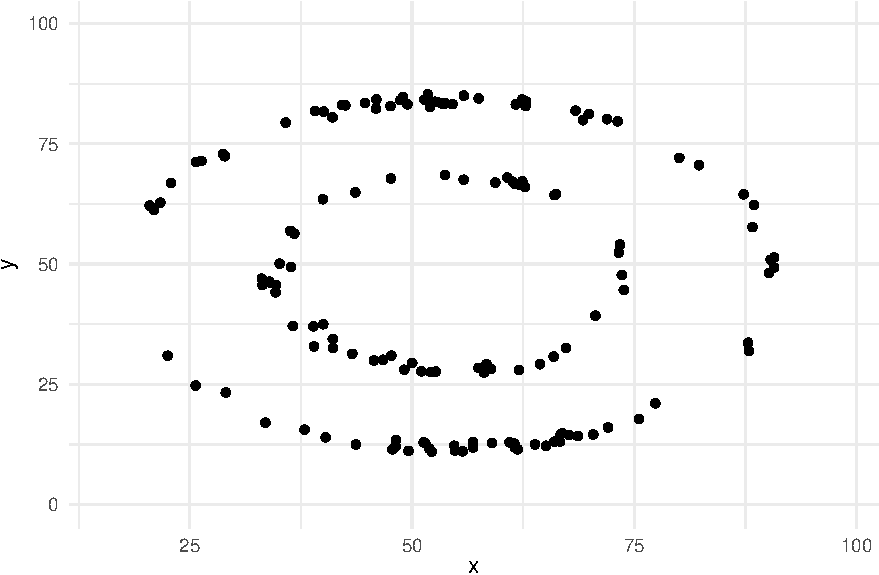
\includegraphics[keepaspectratio]{Hatakeda_Chap03_files/figure-pdf/unnamed-chunk-17-11.pdf}}

\pandocbounded{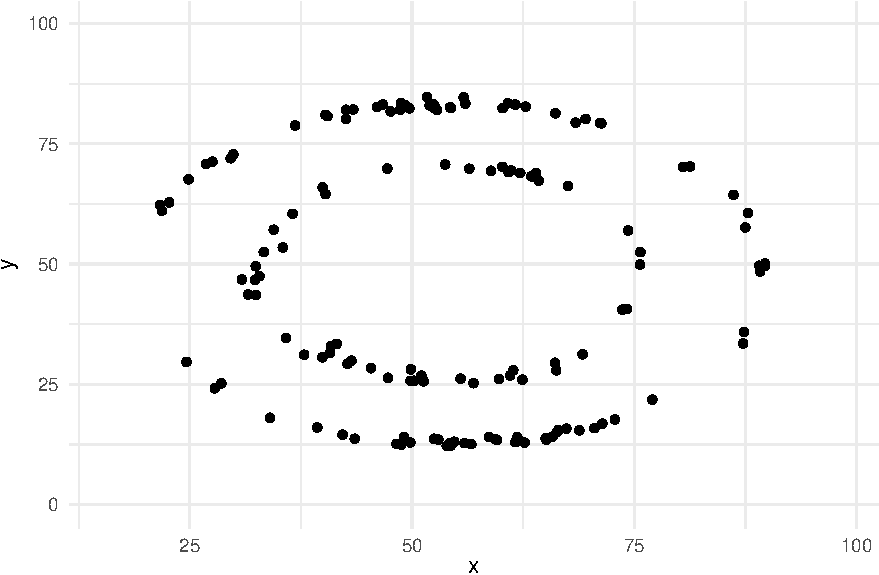
\includegraphics[keepaspectratio]{Hatakeda_Chap03_files/figure-pdf/unnamed-chunk-17-12.pdf}}

\pandocbounded{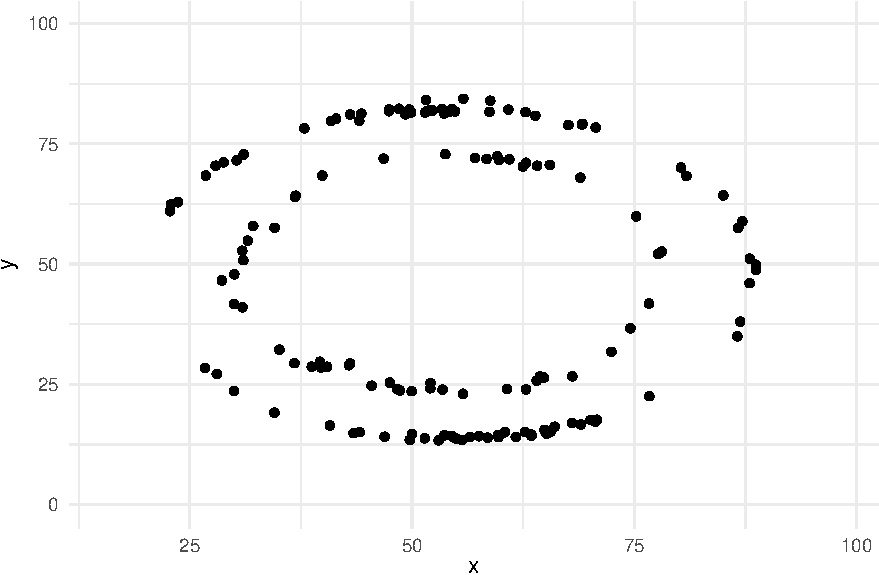
\includegraphics[keepaspectratio]{Hatakeda_Chap03_files/figure-pdf/unnamed-chunk-17-13.pdf}}

\pandocbounded{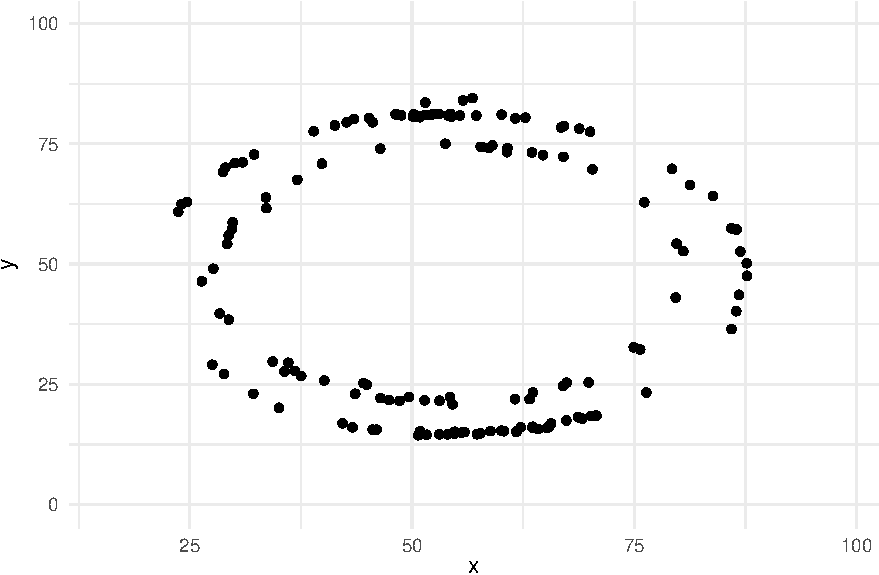
\includegraphics[keepaspectratio]{Hatakeda_Chap03_files/figure-pdf/unnamed-chunk-17-14.pdf}}

\pandocbounded{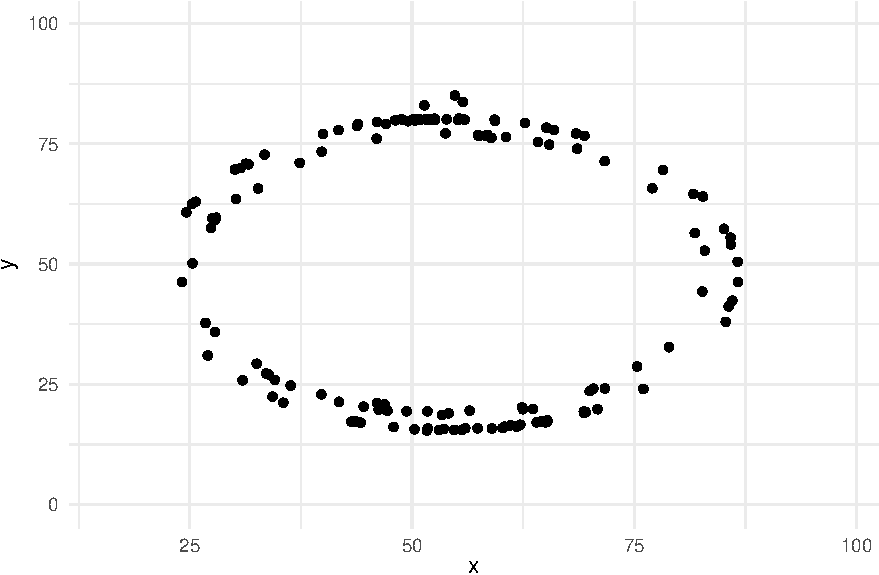
\includegraphics[keepaspectratio]{Hatakeda_Chap03_files/figure-pdf/unnamed-chunk-17-15.pdf}}

\pandocbounded{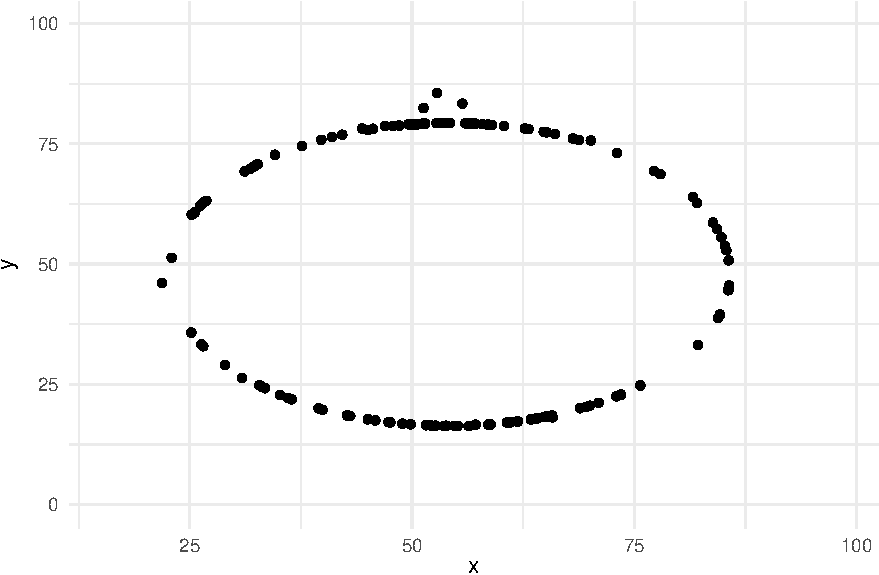
\includegraphics[keepaspectratio]{Hatakeda_Chap03_files/figure-pdf/unnamed-chunk-17-16.pdf}}

\pandocbounded{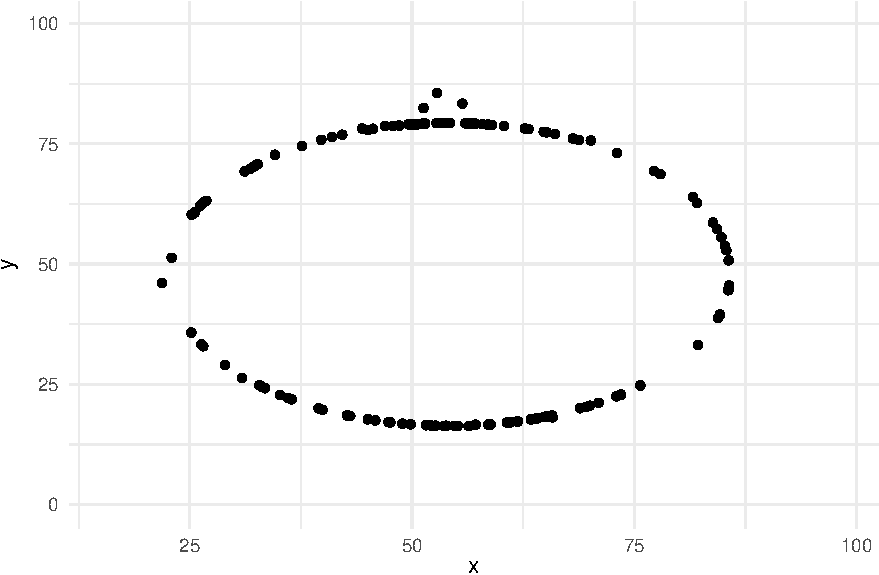
\includegraphics[keepaspectratio]{Hatakeda_Chap03_files/figure-pdf/unnamed-chunk-17-17.pdf}}

\pandocbounded{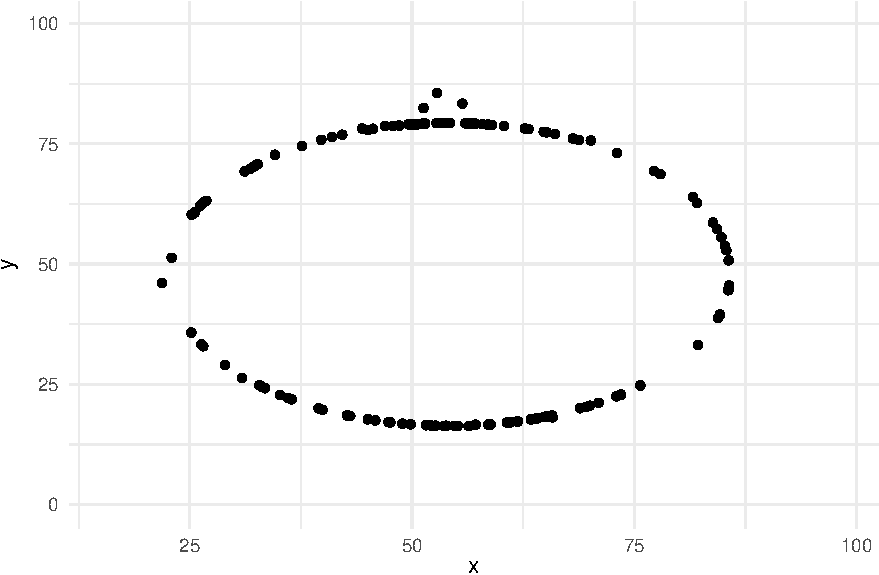
\includegraphics[keepaspectratio]{Hatakeda_Chap03_files/figure-pdf/unnamed-chunk-17-18.pdf}}

\pandocbounded{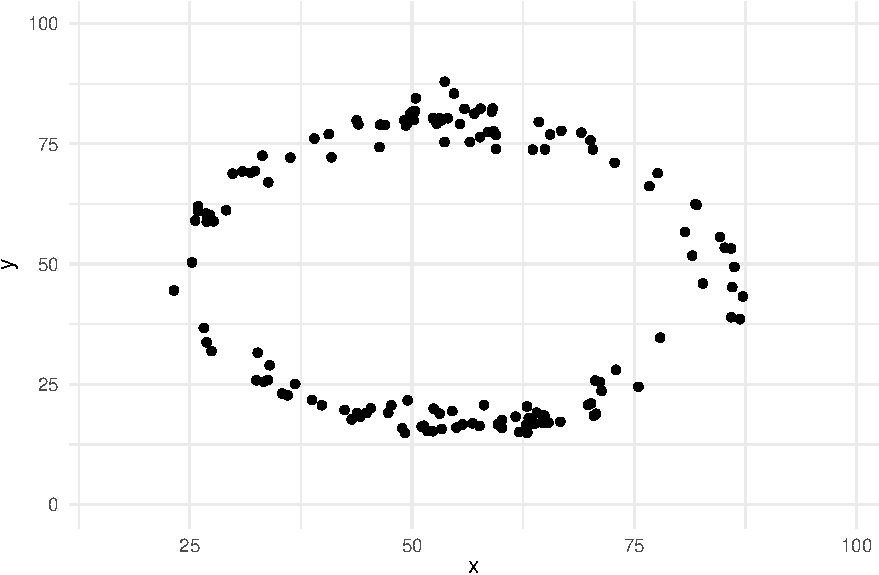
\includegraphics[keepaspectratio]{Hatakeda_Chap03_files/figure-pdf/unnamed-chunk-17-19.pdf}}

\pandocbounded{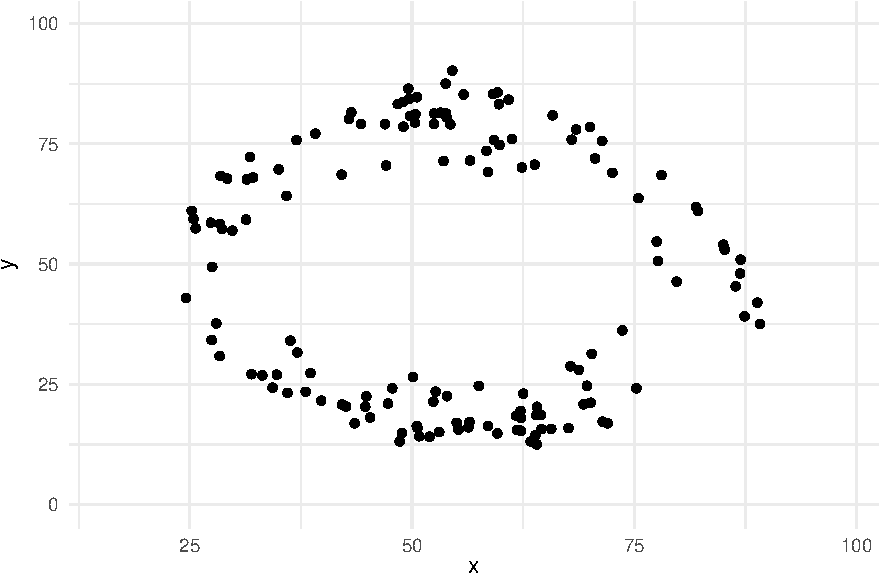
\includegraphics[keepaspectratio]{Hatakeda_Chap03_files/figure-pdf/unnamed-chunk-17-20.pdf}}

\pandocbounded{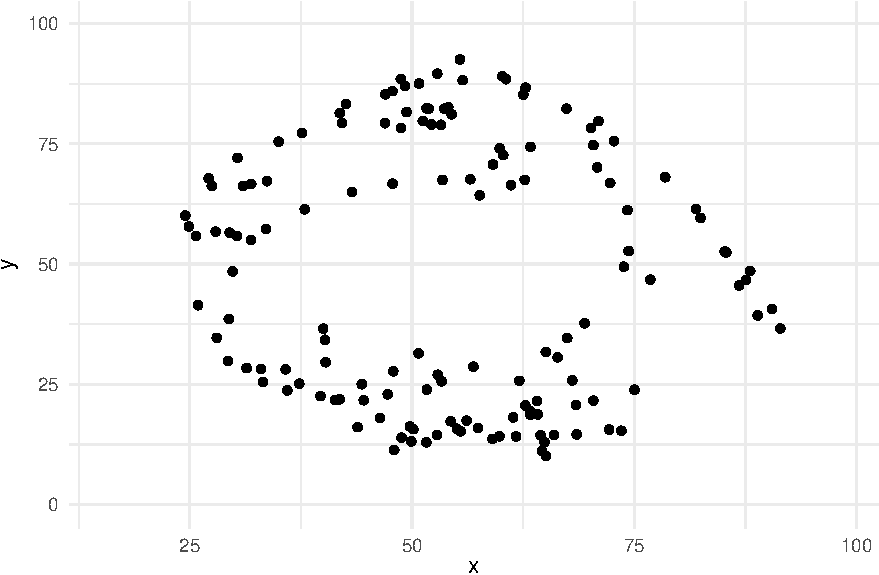
\includegraphics[keepaspectratio]{Hatakeda_Chap03_files/figure-pdf/unnamed-chunk-17-21.pdf}}

\pandocbounded{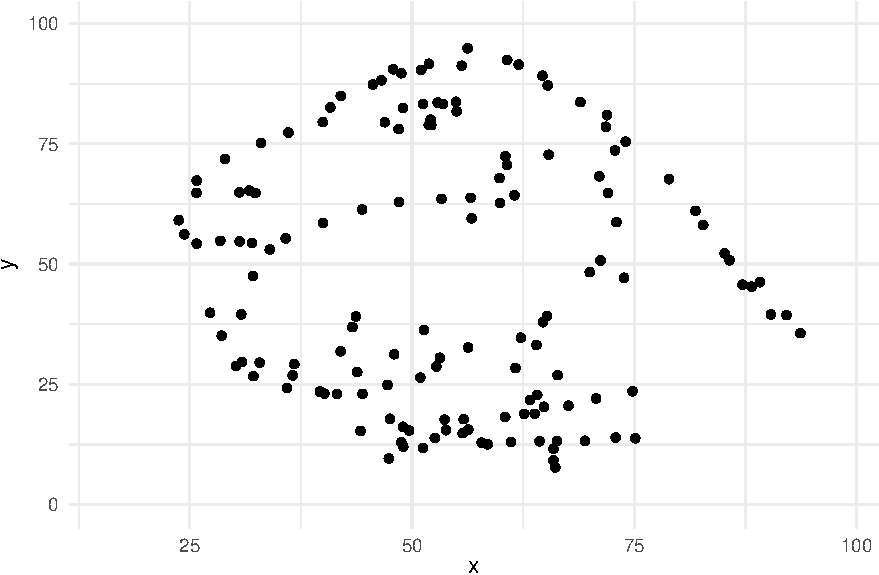
\includegraphics[keepaspectratio]{Hatakeda_Chap03_files/figure-pdf/unnamed-chunk-17-22.pdf}}

\pandocbounded{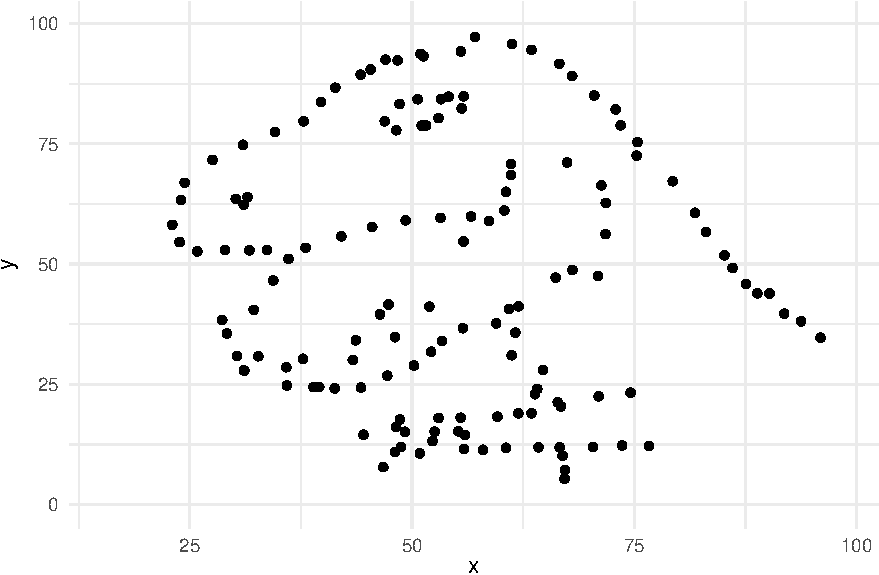
\includegraphics[keepaspectratio]{Hatakeda_Chap03_files/figure-pdf/unnamed-chunk-17-23.pdf}}

\pandocbounded{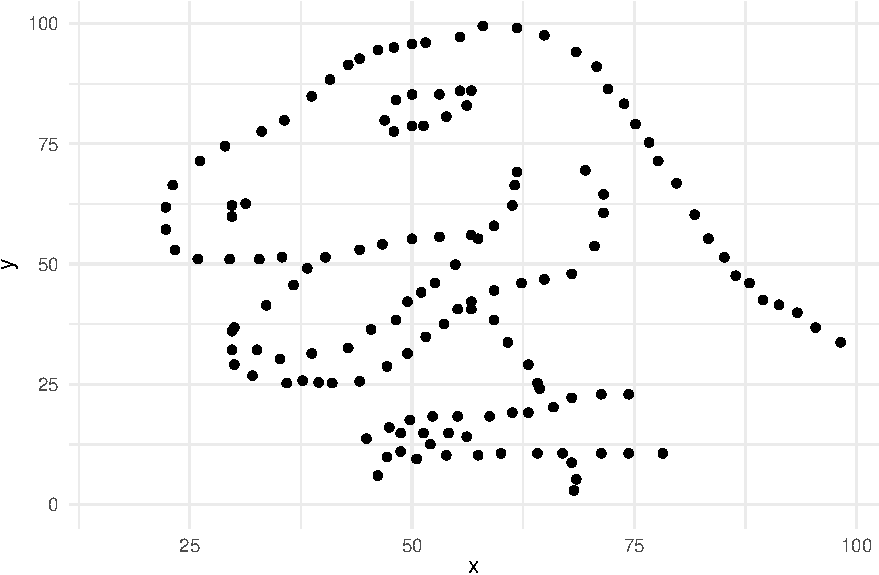
\includegraphics[keepaspectratio]{Hatakeda_Chap03_files/figure-pdf/unnamed-chunk-17-24.pdf}}

\pandocbounded{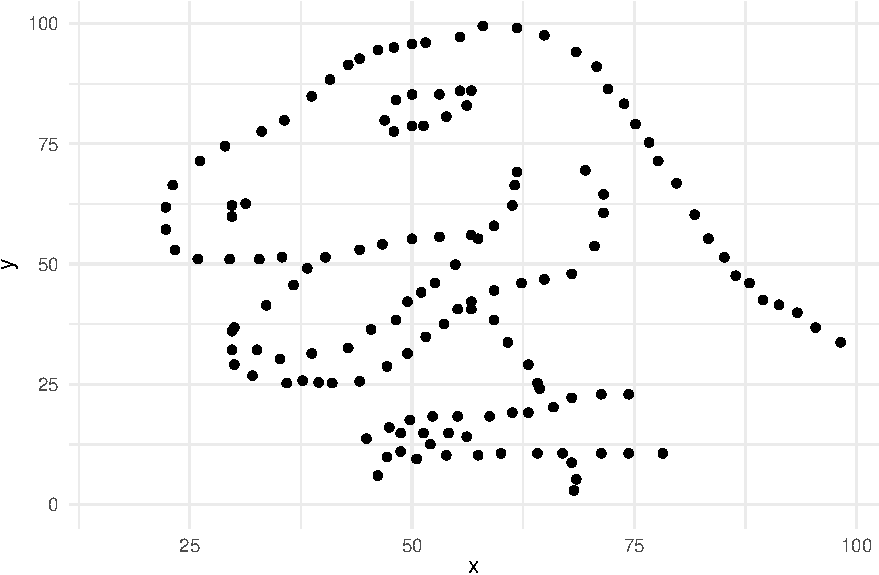
\includegraphics[keepaspectratio]{Hatakeda_Chap03_files/figure-pdf/unnamed-chunk-17-25.pdf}}

\pandocbounded{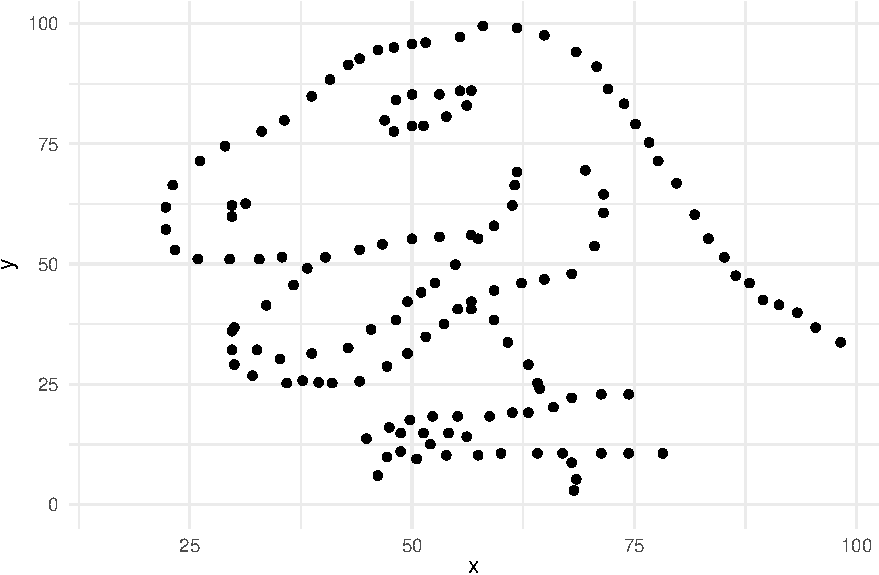
\includegraphics[keepaspectratio]{Hatakeda_Chap03_files/figure-pdf/unnamed-chunk-17-26.pdf}}

\pandocbounded{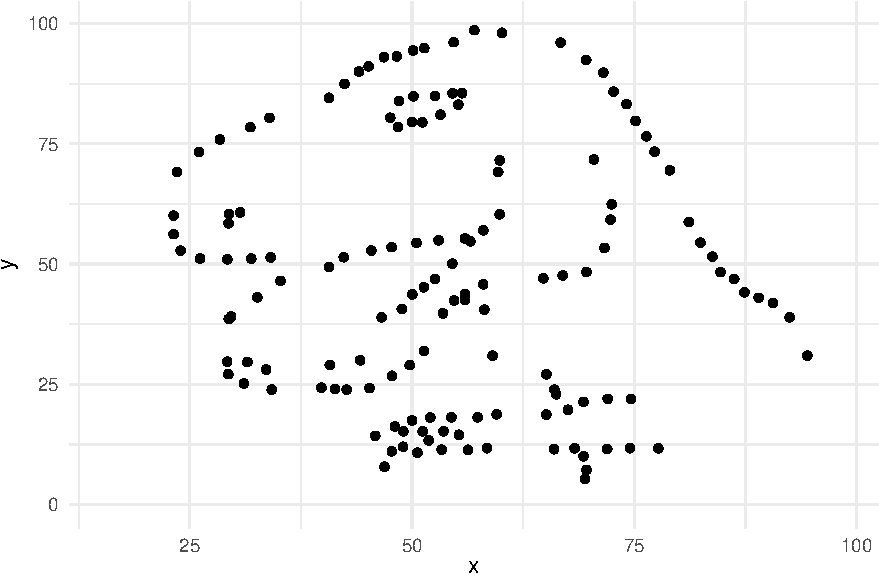
\includegraphics[keepaspectratio]{Hatakeda_Chap03_files/figure-pdf/unnamed-chunk-17-27.pdf}}

\pandocbounded{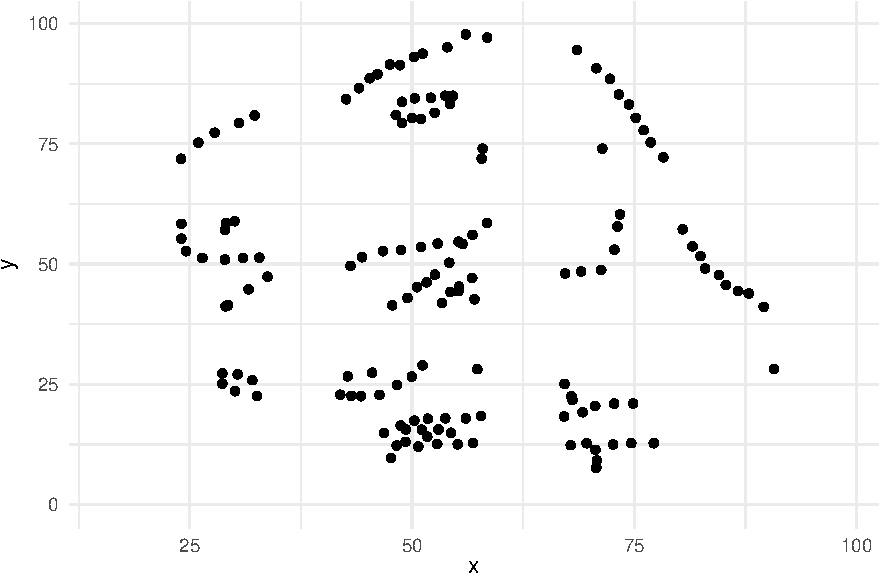
\includegraphics[keepaspectratio]{Hatakeda_Chap03_files/figure-pdf/unnamed-chunk-17-28.pdf}}

\pandocbounded{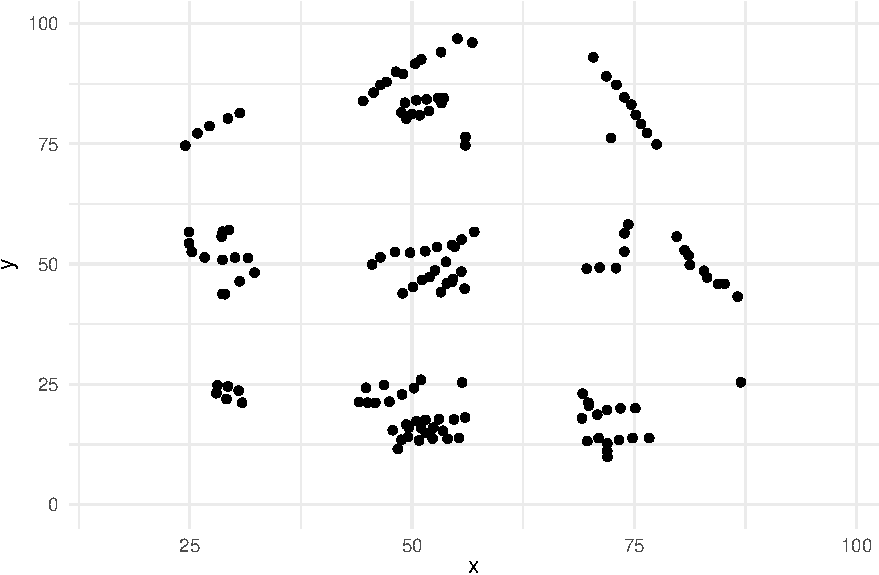
\includegraphics[keepaspectratio]{Hatakeda_Chap03_files/figure-pdf/unnamed-chunk-17-29.pdf}}

\pandocbounded{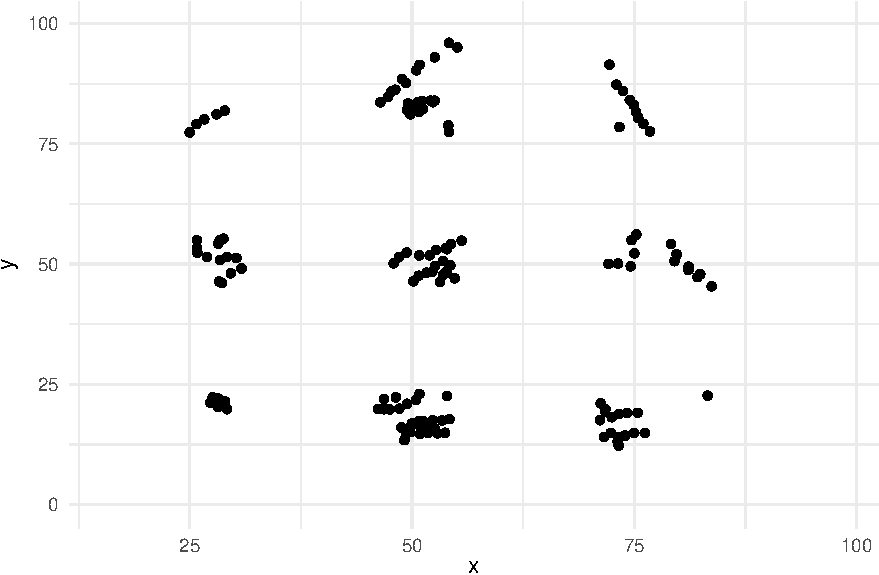
\includegraphics[keepaspectratio]{Hatakeda_Chap03_files/figure-pdf/unnamed-chunk-17-30.pdf}}

\pandocbounded{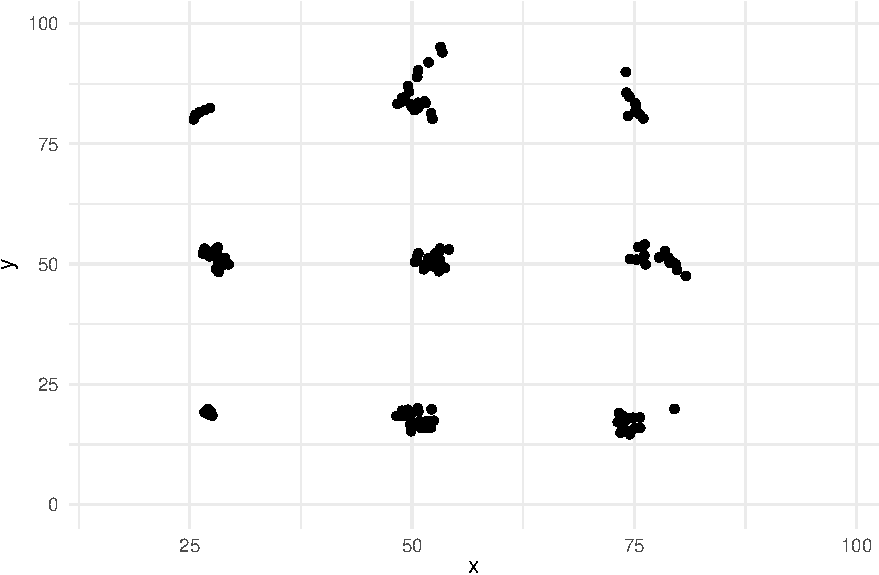
\includegraphics[keepaspectratio]{Hatakeda_Chap03_files/figure-pdf/unnamed-chunk-17-31.pdf}}

\pandocbounded{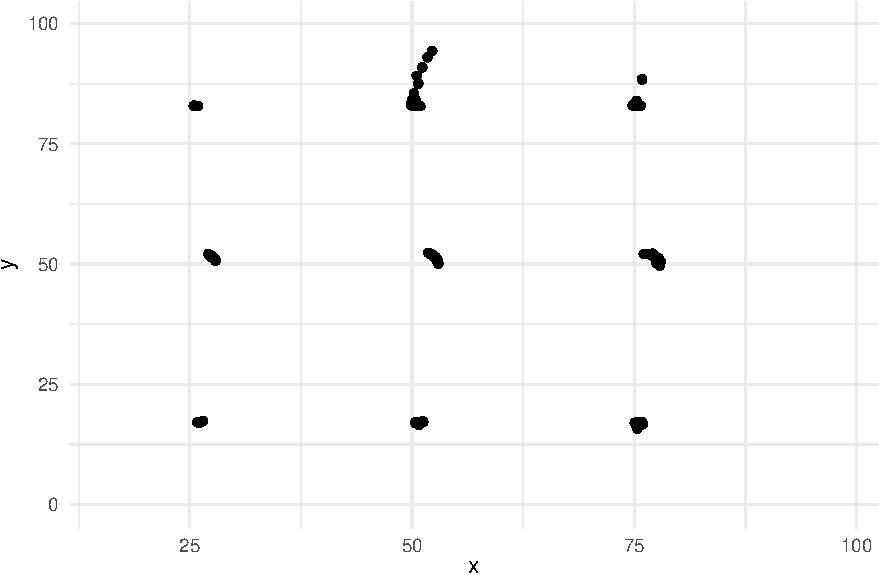
\includegraphics[keepaspectratio]{Hatakeda_Chap03_files/figure-pdf/unnamed-chunk-17-32.pdf}}

\pandocbounded{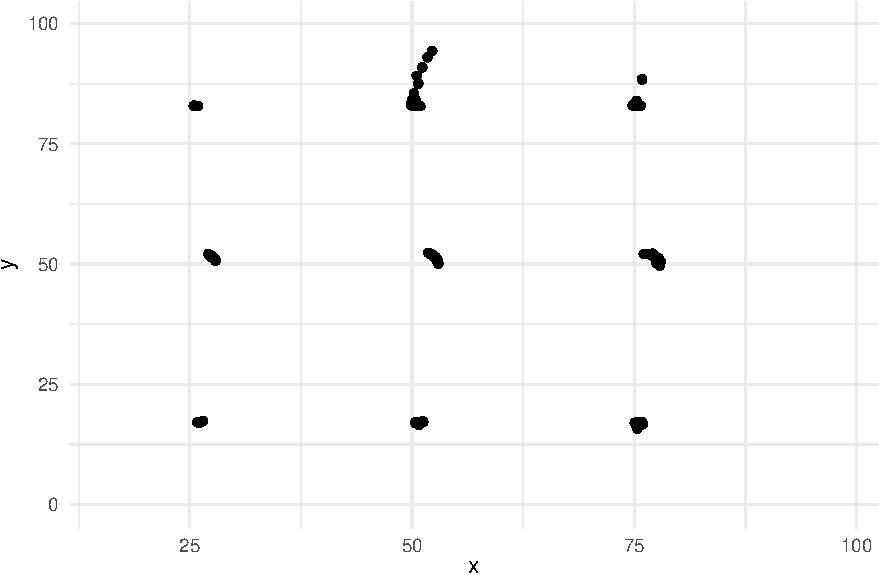
\includegraphics[keepaspectratio]{Hatakeda_Chap03_files/figure-pdf/unnamed-chunk-17-33.pdf}}

\pandocbounded{\includegraphics[keepaspectratio]{Hatakeda_Chap03_files/figure-pdf/unnamed-chunk-17-34.pdf}}

\pandocbounded{\includegraphics[keepaspectratio]{Hatakeda_Chap03_files/figure-pdf/unnamed-chunk-17-35.pdf}}

\pandocbounded{\includegraphics[keepaspectratio]{Hatakeda_Chap03_files/figure-pdf/unnamed-chunk-17-36.pdf}}

\pandocbounded{\includegraphics[keepaspectratio]{Hatakeda_Chap03_files/figure-pdf/unnamed-chunk-17-37.pdf}}

\pandocbounded{\includegraphics[keepaspectratio]{Hatakeda_Chap03_files/figure-pdf/unnamed-chunk-17-38.pdf}}

\pandocbounded{\includegraphics[keepaspectratio]{Hatakeda_Chap03_files/figure-pdf/unnamed-chunk-17-39.pdf}}

\pandocbounded{\includegraphics[keepaspectratio]{Hatakeda_Chap03_files/figure-pdf/unnamed-chunk-17-40.pdf}}

\pandocbounded{\includegraphics[keepaspectratio]{Hatakeda_Chap03_files/figure-pdf/unnamed-chunk-17-41.pdf}}

\pandocbounded{\includegraphics[keepaspectratio]{Hatakeda_Chap03_files/figure-pdf/unnamed-chunk-17-42.pdf}}

\pandocbounded{\includegraphics[keepaspectratio]{Hatakeda_Chap03_files/figure-pdf/unnamed-chunk-17-43.pdf}}

\pandocbounded{\includegraphics[keepaspectratio]{Hatakeda_Chap03_files/figure-pdf/unnamed-chunk-17-44.pdf}}

\pandocbounded{\includegraphics[keepaspectratio]{Hatakeda_Chap03_files/figure-pdf/unnamed-chunk-17-45.pdf}}

\pandocbounded{\includegraphics[keepaspectratio]{Hatakeda_Chap03_files/figure-pdf/unnamed-chunk-17-46.pdf}}

\pandocbounded{\includegraphics[keepaspectratio]{Hatakeda_Chap03_files/figure-pdf/unnamed-chunk-17-47.pdf}}

\pandocbounded{\includegraphics[keepaspectratio]{Hatakeda_Chap03_files/figure-pdf/unnamed-chunk-17-48.pdf}}

\pandocbounded{\includegraphics[keepaspectratio]{Hatakeda_Chap03_files/figure-pdf/unnamed-chunk-17-49.pdf}}

\pandocbounded{\includegraphics[keepaspectratio]{Hatakeda_Chap03_files/figure-pdf/unnamed-chunk-17-50.pdf}}

\pandocbounded{\includegraphics[keepaspectratio]{Hatakeda_Chap03_files/figure-pdf/unnamed-chunk-17-51.pdf}}

\pandocbounded{\includegraphics[keepaspectratio]{Hatakeda_Chap03_files/figure-pdf/unnamed-chunk-17-52.pdf}}

\pandocbounded{\includegraphics[keepaspectratio]{Hatakeda_Chap03_files/figure-pdf/unnamed-chunk-17-53.pdf}}

\pandocbounded{\includegraphics[keepaspectratio]{Hatakeda_Chap03_files/figure-pdf/unnamed-chunk-17-54.pdf}}

\pandocbounded{\includegraphics[keepaspectratio]{Hatakeda_Chap03_files/figure-pdf/unnamed-chunk-17-55.pdf}}

\pandocbounded{\includegraphics[keepaspectratio]{Hatakeda_Chap03_files/figure-pdf/unnamed-chunk-17-56.pdf}}

\pandocbounded{\includegraphics[keepaspectratio]{Hatakeda_Chap03_files/figure-pdf/unnamed-chunk-17-57.pdf}}

\pandocbounded{\includegraphics[keepaspectratio]{Hatakeda_Chap03_files/figure-pdf/unnamed-chunk-17-58.pdf}}

\pandocbounded{\includegraphics[keepaspectratio]{Hatakeda_Chap03_files/figure-pdf/unnamed-chunk-17-59.pdf}}

\pandocbounded{\includegraphics[keepaspectratio]{Hatakeda_Chap03_files/figure-pdf/unnamed-chunk-17-60.pdf}}

\pandocbounded{\includegraphics[keepaspectratio]{Hatakeda_Chap03_files/figure-pdf/unnamed-chunk-17-61.pdf}}

\pandocbounded{\includegraphics[keepaspectratio]{Hatakeda_Chap03_files/figure-pdf/unnamed-chunk-17-62.pdf}}

\pandocbounded{\includegraphics[keepaspectratio]{Hatakeda_Chap03_files/figure-pdf/unnamed-chunk-17-63.pdf}}

\pandocbounded{\includegraphics[keepaspectratio]{Hatakeda_Chap03_files/figure-pdf/unnamed-chunk-17-64.pdf}}

\pandocbounded{\includegraphics[keepaspectratio]{Hatakeda_Chap03_files/figure-pdf/unnamed-chunk-17-65.pdf}}

\pandocbounded{\includegraphics[keepaspectratio]{Hatakeda_Chap03_files/figure-pdf/unnamed-chunk-17-66.pdf}}

\pandocbounded{\includegraphics[keepaspectratio]{Hatakeda_Chap03_files/figure-pdf/unnamed-chunk-17-67.pdf}}

\pandocbounded{\includegraphics[keepaspectratio]{Hatakeda_Chap03_files/figure-pdf/unnamed-chunk-17-68.pdf}}

\pandocbounded{\includegraphics[keepaspectratio]{Hatakeda_Chap03_files/figure-pdf/unnamed-chunk-17-69.pdf}}

\pandocbounded{\includegraphics[keepaspectratio]{Hatakeda_Chap03_files/figure-pdf/unnamed-chunk-17-70.pdf}}

\pandocbounded{\includegraphics[keepaspectratio]{Hatakeda_Chap03_files/figure-pdf/unnamed-chunk-17-71.pdf}}

\pandocbounded{\includegraphics[keepaspectratio]{Hatakeda_Chap03_files/figure-pdf/unnamed-chunk-17-72.pdf}}

\pandocbounded{\includegraphics[keepaspectratio]{Hatakeda_Chap03_files/figure-pdf/unnamed-chunk-17-73.pdf}}

\pandocbounded{\includegraphics[keepaspectratio]{Hatakeda_Chap03_files/figure-pdf/unnamed-chunk-17-74.pdf}}

\pandocbounded{\includegraphics[keepaspectratio]{Hatakeda_Chap03_files/figure-pdf/unnamed-chunk-17-75.pdf}}

\pandocbounded{\includegraphics[keepaspectratio]{Hatakeda_Chap03_files/figure-pdf/unnamed-chunk-17-76.pdf}}

\pandocbounded{\includegraphics[keepaspectratio]{Hatakeda_Chap03_files/figure-pdf/unnamed-chunk-17-77.pdf}}

\pandocbounded{\includegraphics[keepaspectratio]{Hatakeda_Chap03_files/figure-pdf/unnamed-chunk-17-78.pdf}}

\pandocbounded{\includegraphics[keepaspectratio]{Hatakeda_Chap03_files/figure-pdf/unnamed-chunk-17-79.pdf}}

\pandocbounded{\includegraphics[keepaspectratio]{Hatakeda_Chap03_files/figure-pdf/unnamed-chunk-17-80.pdf}}

\pandocbounded{\includegraphics[keepaspectratio]{Hatakeda_Chap03_files/figure-pdf/unnamed-chunk-17-81.pdf}}

\pandocbounded{\includegraphics[keepaspectratio]{Hatakeda_Chap03_files/figure-pdf/unnamed-chunk-17-82.pdf}}

\pandocbounded{\includegraphics[keepaspectratio]{Hatakeda_Chap03_files/figure-pdf/unnamed-chunk-17-83.pdf}}

\pandocbounded{\includegraphics[keepaspectratio]{Hatakeda_Chap03_files/figure-pdf/unnamed-chunk-17-84.pdf}}

\pandocbounded{\includegraphics[keepaspectratio]{Hatakeda_Chap03_files/figure-pdf/unnamed-chunk-17-85.pdf}}

\pandocbounded{\includegraphics[keepaspectratio]{Hatakeda_Chap03_files/figure-pdf/unnamed-chunk-17-86.pdf}}

\pandocbounded{\includegraphics[keepaspectratio]{Hatakeda_Chap03_files/figure-pdf/unnamed-chunk-17-87.pdf}}

\pandocbounded{\includegraphics[keepaspectratio]{Hatakeda_Chap03_files/figure-pdf/unnamed-chunk-17-88.pdf}}

\pandocbounded{\includegraphics[keepaspectratio]{Hatakeda_Chap03_files/figure-pdf/unnamed-chunk-17-89.pdf}}

\pandocbounded{\includegraphics[keepaspectratio]{Hatakeda_Chap03_files/figure-pdf/unnamed-chunk-17-90.pdf}}

\pandocbounded{\includegraphics[keepaspectratio]{Hatakeda_Chap03_files/figure-pdf/unnamed-chunk-17-91.pdf}}

\pandocbounded{\includegraphics[keepaspectratio]{Hatakeda_Chap03_files/figure-pdf/unnamed-chunk-17-92.pdf}}

\pandocbounded{\includegraphics[keepaspectratio]{Hatakeda_Chap03_files/figure-pdf/unnamed-chunk-17-93.pdf}}

\pandocbounded{\includegraphics[keepaspectratio]{Hatakeda_Chap03_files/figure-pdf/unnamed-chunk-17-94.pdf}}

\pandocbounded{\includegraphics[keepaspectratio]{Hatakeda_Chap03_files/figure-pdf/unnamed-chunk-17-95.pdf}}

\pandocbounded{\includegraphics[keepaspectratio]{Hatakeda_Chap03_files/figure-pdf/unnamed-chunk-17-96.pdf}}

\pandocbounded{\includegraphics[keepaspectratio]{Hatakeda_Chap03_files/figure-pdf/unnamed-chunk-17-97.pdf}}

\pandocbounded{\includegraphics[keepaspectratio]{Hatakeda_Chap03_files/figure-pdf/unnamed-chunk-17-98.pdf}}

\pandocbounded{\includegraphics[keepaspectratio]{Hatakeda_Chap03_files/figure-pdf/unnamed-chunk-17-99.pdf}}

\pandocbounded{\includegraphics[keepaspectratio]{Hatakeda_Chap03_files/figure-pdf/unnamed-chunk-17-100.pdf}}

この散布図のデータの基本統計量はほぼ同じで,相関係数はほぼ\(0\)のデータですが,実際に散布図として可視化してみると全く異なるデータであることがわかります。
つまりは,手元のデータは一度可視化して,そのデータの特徴をつかむことが重要なのです。

\section{変数のアフィン変換}\label{ux5909ux6570ux306eux30a2ux30d5ux30a3ux30f3ux5909ux63db}

線形変換(linear transformation)とは,線形性をもつ変換で, \[
f(\boldsymbol{x}) = \boldsymbol{A}\boldsymbol{x}
\] と表し,線形変換は,

\begin{enumerate}
\def\labelenumi{\arabic{enumi}.}
\tightlist
\item
  直線を維持したまま,
\item
  原点を固定
\end{enumerate}

した変換となります。この線形変換\(f\)に平行移動\(g\)を合成した変換を\textbf{アフィン変換}(affine
transformation)といいます。

確率変数の一次変換あるいは線形変換、より一般的にはアフィン変換について学習します。
一般に確率変数\(X\)のアフィン変換は以下のように表されます。

\[
\begin{aligned}
y = f \circ g (\boldsymbol{x}) = \boldsymbol{A}\boldsymbol{x} + \boldsymbol{b}
\end{aligned}
\]

以下では,ある確率変数\(X\)に対して,行列\(\boldsymbol{A}\)がスカラー\(a\),ベクトル\(\boldsymbol{b}\)がスカラー\(b\)の場合を考えます。
つまり, \[
Y = a X + b
\] である場合について考えます。
このとき,変換後の確率変数\(Y\)の期待値と分散は以下のようになります。

\[
\begin{aligned}
\mathbb{E}[Y] &= a\mathbb{E}[X] + b \\
\mathbb{V}[Y] &= a^2 \mathbb{V}[X] \\
\mathbb{SD}[Y] &= |a| \mathbb{SD}[X]
\end{aligned}
\]

以下の例で確認してみましょう。
従業員9名の1ヶ月の労働時間\(X\)が以下の表に示されている。

\begin{Shaded}
\begin{Highlighting}[]
\NormalTok{labor }\OtherTok{\textless{}{-}} \FunctionTok{data.frame}\NormalTok{(}
\NormalTok{    従業員 }\OtherTok{=} \FunctionTok{c}\NormalTok{(}\StringTok{"A"}\NormalTok{,}\StringTok{"B"}\NormalTok{,}\StringTok{"C"}\NormalTok{,}\StringTok{"D"}\NormalTok{,}\StringTok{"E"}\NormalTok{,}\StringTok{"F"}\NormalTok{,}\StringTok{"G"}\NormalTok{,}\StringTok{"H"}\NormalTok{,}\StringTok{"I"}\NormalTok{),}
\NormalTok{    労働時間 }\OtherTok{=} \FunctionTok{c}\NormalTok{(}\DecValTok{30}\NormalTok{,}\DecValTok{45}\NormalTok{,}\DecValTok{50}\NormalTok{,}\DecValTok{35}\NormalTok{,}\DecValTok{60}\NormalTok{,}\DecValTok{70}\NormalTok{,}\DecValTok{55}\NormalTok{,}\DecValTok{60}\NormalTok{,}\DecValTok{45}\NormalTok{)}
\NormalTok{)}
\NormalTok{knitr}\SpecialCharTok{::}\FunctionTok{kable}\NormalTok{(}\FunctionTok{t}\NormalTok{(labor), }\AttributeTok{booktabs =} \ConstantTok{TRUE}\NormalTok{)}
\end{Highlighting}
\end{Shaded}

\begin{longtable}[]{@{}llllllllll@{}}
\toprule\noalign{}
\endhead
\bottomrule\noalign{}
\endlastfoot
従業員 & A & B & C & D & E & F & G & H & I \\
労働時間 & 30 & 45 & 50 & 35 & 60 & 70 & 55 & 60 & 45 \\
\end{longtable}

総賃金\(Y_2\)は毎月の固定給100千円に時間給\(Y_1\)(時給3千円)を合わせた額として支給される。
すなわち,\(Y_2 = 100 + Y_1 = 100 + 3X\)の関係が成立している。
したがって,各従業員の労働時間と賃金は以下の通りとなる。

\begin{Shaded}
\begin{Highlighting}[]
\NormalTok{labor }\OtherTok{\textless{}{-}}\NormalTok{ labor }\SpecialCharTok{\%\textgreater{}\%}
    \FunctionTok{mutate}\NormalTok{(}
\NormalTok{        時間給 }\OtherTok{=}\NormalTok{ 労働時間 }\SpecialCharTok{*} \DecValTok{3}\NormalTok{,}
\NormalTok{        総賃金 }\OtherTok{=} \DecValTok{100} \SpecialCharTok{+}\NormalTok{ 時間給}
\NormalTok{    )}
\NormalTok{knitr}\SpecialCharTok{::}\FunctionTok{kable}\NormalTok{(}\FunctionTok{t}\NormalTok{(labor), }\AttributeTok{booktabs =} \ConstantTok{TRUE}\NormalTok{)}
\end{Highlighting}
\end{Shaded}

\begin{longtable}[]{@{}llllllllll@{}}
\toprule\noalign{}
\endhead
\bottomrule\noalign{}
\endlastfoot
従業員 & A & B & C & D & E & F & G & H & I \\
労働時間 & 30 & 45 & 50 & 35 & 60 & 70 & 55 & 60 & 45 \\
時間給 & 90 & 135 & 150 & 105 & 180 & 210 & 165 & 180 & 135 \\
総賃金 & 190 & 235 & 250 & 205 & 280 & 310 & 265 & 280 & 235 \\
\end{longtable}

この表からわかることは,\(Y_1=3X\)であることから,\(Y_1\)の標本平均と標本標準偏差はともに\(X\)の標本平均と標本標準偏差の3倍になっている,ということです。
つまり,標本平均と標本標準偏差はともに比例的に変化していることがわかります。

このデータを元に,労働時間,時間給,総賃金の標本平均や標本標準偏差を計算してみましょう。

\begin{Shaded}
\begin{Highlighting}[]
\NormalTok{labor\_summary }\OtherTok{\textless{}{-}}\NormalTok{ labor }\SpecialCharTok{\%\textgreater{}\%}
    \FunctionTok{summarise}\NormalTok{(}
\NormalTok{        平均 }\OtherTok{=} \FunctionTok{c}\NormalTok{(}\FunctionTok{mean}\NormalTok{(労働時間), }\FunctionTok{mean}\NormalTok{(時間給), }\FunctionTok{mean}\NormalTok{(総賃金)),}
\NormalTok{        標準偏差 }\OtherTok{=} \FunctionTok{c}\NormalTok{(}\FunctionTok{sd}\NormalTok{(労働時間), }\FunctionTok{sd}\NormalTok{(時間給), }\FunctionTok{sd}\NormalTok{(総賃金))}
\NormalTok{    )}
\NormalTok{labor\_summary}\SpecialCharTok{$}\NormalTok{変数名 }\OtherTok{\textless{}{-}} \FunctionTok{c}\NormalTok{(}\StringTok{"労働時間"}\NormalTok{, }\StringTok{"時間給"}\NormalTok{, }\StringTok{"総賃金"}\NormalTok{)}
\NormalTok{labor\_summary }\OtherTok{\textless{}{-}}\NormalTok{ labor\_summary }\SpecialCharTok{\%\textgreater{}\%}
    \FunctionTok{select}\NormalTok{(変数名, 平均, 標準偏差)}
\NormalTok{knitr}\SpecialCharTok{::}\FunctionTok{kable}\NormalTok{(labor\_summary, }\AttributeTok{booktabs =} \ConstantTok{TRUE}\NormalTok{, }\AttributeTok{digits =} \DecValTok{2}\NormalTok{)}
\end{Highlighting}
\end{Shaded}

\begin{longtable}[]{@{}lrr@{}}
\toprule\noalign{}
変数名 & 平均 & 標準偏差 \\
\midrule\noalign{}
\endhead
\bottomrule\noalign{}
\endlastfoot
労働時間 & 50 & 12.75 \\
時間給 & 150 & 38.24 \\
総賃金 & 250 & 38.24 \\
\end{longtable}

総賃金は\(Y_2 = 100 + Y_1\)であるため,総賃金\(Y_2\)の標本平均は時間給\(Y_1\)の標本平均に\(100\)を加えたものになります。
また総賃金\(Y_2\)の標本標準偏差は、時間給\(Y_1\)と同じである。

\section{変数の線形結合}\label{ux5909ux6570ux306eux7ddaux5f62ux7d50ux5408}

より一般的に線形結合について考えてみましょう。
いま、\(k\)個の変数\(X_1,\dots ,X_k\)から一次結合\(Y = c_0 + c_1 X_1 + \cdots + c_k X_k\)で表される変数\(Y\)において(ただし\(c\)はパラメータ),データから計算される変数\(Y\)の標本平均,標本分散(標本標準偏差)に対して次の関係が成立します。

\[
\begin{aligned}
\mathbb{E}[Y] &= \mathbb{E}[c_0 + c_1 X_1 + \cdots + c_k X_k ]\\
            &= c_0 + c_1 \mathbb{E}[X_1] + \cdots + c_k\mathbb{E}[ X_k ] \\
            &= c_0 + c_1 \bar{X}_1 + \cdots + c_k\bar{X}_k \\
\mathbb{V}[Y] &= \mathbb{V}[c_0 + c_1 X_1 + \cdots + c_k X_k ]\\
&= c_0 + \mathbb{V}[c_1 X_1] + \cdots + \mathbb{V}[c_k X_k ] + \sum _{i \not = j}^k  \sum _{j \not = i}^k c_i c_j s_{ij}(X_i,X_j)\\
&= c_0 + c_1^2\mathbb{V}[X_1] + \cdots + c_k^2\mathbb{V}[X_k ] + \sum _{i \not = j}^k  \sum _{j \not = i}^k c_i c_j s_{ij}(X_i,X_j)
\mathbb{V}[Y] &= a^2 \mathbb{V}[X] \\
\mathbb{SD}[Y] &= |a| \mathbb{SD}[X]
\end{aligned}
\]

\[
\begin{aligned}
\bar Y &= c_0 + c_1 \bar X_1 + \cdots + c_k \bar X_k \\
s^2[Y] &= c_1^2 s^2[X_1] + \cdots + c_k^2 s^2[X_k] + \sum _{i \not = j}^k \sum _{j \not = i}^k c_i c_j s_{ij}(X_i,X_j)
\end{aligned}
\]

ここで,\(\bar X_i\),\(s^2[X_i]\),
\(s_{ij}(X_i,X_j)\)はそれぞれ標本平均,標本分散,標本共分散を表す。

\(k=2\)の場合,

\[
\begin{aligned}
\bar Y &= c_0 + c_1 \bar X_1 + c_2 \bar X_2 \\
s^2[Y] &= c_1^2 s^2[X_1] + c_2^2 s^2[X_2] + 2 c_1 c_2 s_{12}(X_1,X_2)
\end{aligned}
\] となる。

\begin{tcolorbox}[enhanced jigsaw, colframe=quarto-callout-warning-color-frame, breakable, rightrule=.15mm, coltitle=black, title=\textcolor{quarto-callout-warning-color}{\faExclamationTriangle}\hspace{0.5em}{例2}, colbacktitle=quarto-callout-warning-color!10!white, leftrule=.75mm, colback=white, left=2mm, arc=.35mm, opacityback=0, titlerule=0mm, toptitle=1mm, bottomtitle=1mm, bottomrule=.15mm, toprule=.15mm, opacitybacktitle=0.6]

\(k=2\)のケースで,\(Y=0.5X_1 + 0.5 X_2\)の期待値および分散を求める。
ただし,\(\bar X_1 = 0.07\),\(s^2[X_1] = 1.48\),\(\bar X _2 = -0.02\),\(s^2 [X_2] = 1.46\)である。

\begin{itemize}
\item
  無相関(\(s _{ij} (X_i,X_j) = 0\))のケース \[
    \begin{aligned}
    \bar Y   &= 0.5 \times 0.07 + 0.5 \times - 0.02 = 0.025\\
    s^2 [Y]  &= 0.5^2 \times 1.48 + 0.5^2 \times 1.46 + 2 \times 0.5 \times 0.5 \times 0 = 0.735
    \end{aligned}
    \]

  \(Y\)の分散は,\(X_1\)と\(X_2\)の分散よりも小さい。
\item
  負の相関(\$s \_\{ij\}(X\_i,X\_j) = -1.46 \$)のケース

  \[
    \begin{aligned}
    \bar Y   &= 0.5 \times 0.07 + 0.5 \times - 0.02 = 0.025\\
    s^2 [Y]  &= 0.5^2 \times 1.48 + 0.5^2 \times 1.46 + 2 \times 0.5 \times 0.5 \times -1.46 = 0.005
    \end{aligned}
    \]

  \(Y\)の分散は,\(X_1\)と\(X_2\)の分散よりも小さい。
\end{itemize}

\(X_1\)と\(X_2\)の共分散は,\(Y\)の分散に影響を与える。

\end{tcolorbox}

\bookmarksetup{startatroot}

\chapter{効用}\label{ux52b9ux7528}

いままでで、確率と統計の基礎を学習したので、つぎは効用について学習します。
次章から学ぶポートフォリオ理論では、投資家と投資対象の2つをモデル化し、最適な投資意思決定について考えます。

投資対象として株式や債券を中心に学習しますが、それらの投資対象をモデル化するさいに重要なことは、投資対象がもつリスクをどのように捉えるか、ということです。
そこでは、確率分布を用いてリスクをモデル化しました。つまり、投資対象がもたらすリターンのばらつきが大きい、つまり分散(あるいは標準偏差)が大きいとき、その投資対象はリスクが高い、とします。

つぎに投資対象に投資する主体である投資家の投資対象に対する選好をモデル化する必要があります。
ここに\textbf{効用}が登場します。

この節では,以下の項目について学習します。

\begin{itemize}
\tightlist
\item
  効用関数
\item
  リスク態度・リスク回避度
\item
  確実性等価
\item
  リスクプレミアム
\end{itemize}

ファイナンスはリスクについて考える学問といえます。そして個人が負担するリスクを考える際、個人がリスクに対してどのような態度を持っているのか、を表現する必要があります。
そこで用いられる概念が\textbf{効用}(utility)となります。

株式の例で考えてみましょう。

\begin{tcolorbox}[enhanced jigsaw, colframe=quarto-callout-warning-color-frame, breakable, rightrule=.15mm, coltitle=black, title=\textcolor{quarto-callout-warning-color}{\faExclamationTriangle}\hspace{0.5em}{例1 : 株価}, colbacktitle=quarto-callout-warning-color!10!white, leftrule=.75mm, colback=white, left=2mm, arc=.35mm, opacityback=0, titlerule=0mm, toptitle=1mm, bottomtitle=1mm, bottomrule=.15mm, toprule=.15mm, opacitybacktitle=0.6]

株式Aと株式Bの2銘柄を考えます。
将来起こりうる状態が2つ(\(g\)、\(b\))あり、それぞれの生起確率は\((0.5, 0.5)\)とします。
これらのことは投資家にとって既知であると仮定します。
つまり、将来\(g\)か\(b\)のどちらかが等確率で生じることは知っているけれど、どちらが出るのかはわからない、という状況です。
\textbf{株価は確率変数である}、ということです。

株式Aは状態\(g\)で価格が\(100\)、状態\(b\)で価格が\(50\)となります。
株式Bは状態\(g\)で価格が\(120\)、状態\(b\)で価格が\(40\)となります。

このとき、投資家はどちらの株式を購入するでしょうか?
この投資家は自己の効用が最大になる選択肢を選ぶとします。

\end{tcolorbox}

\begin{figure}[H]

{\centering \includegraphics[width=0.9\linewidth,height=\textheight,keepaspectratio]{Hatakeda_Chap04_files/figure-pdf/tikz-01-1.pdf}

}

\caption{株式投資の例}

\end{figure}%

\begin{figure}[H]

{\centering \includegraphics[width=0.9\linewidth,height=\textheight,keepaspectratio]{Hatakeda_Chap04_files/figure-pdf/tikz-02-1.pdf}

}

\caption{株式投資の例}

\end{figure}%

第3章で学習したの知識を用いて,株式\(A\)と\(B\)の期待値と標準偏差を求めてみましょう。
資産\(A\)と\(B\)の期待値は, \[
\begin{aligned}
\mathbb{E}[A] &= \frac 12 \times 100 + \frac 12 \times 50 = 75\\
\mathbb{E}[B] &= \frac 12 \times 120 + \frac 12 \times 40 = 80
\end{aligned}
\] となり,資産\(B\)の方が期待値が大きいことがわかります。
つぎに標準偏差を計算してみると, \[
\begin{aligned}
\sigma  [A] &= \sqrt{ \frac 12 \times (100  - 75)^2 + \frac 12 \times (50 - 75)^2} = 25\\
\sigma  [B] &= \sqrt{ \frac 12 \times (120  - 80)^2 + \frac 12 \times (40 - 80)^2} = 40
\end{aligned}
\] となり,資産\(B\)の方が標準偏差が大きいことがわかります。
資産価格の標準偏差や分散を,\emph{リスク}(risk)や\emph{ボラティリティ}(volatility)とよぶことがあります。
つまり,資産\(B\)は期待リターンが高いが,リスクも高い投資先であることがわかりました。

\section{効用関数}\label{ux52b9ux7528ux95a2ux6570}

例2より,株式\(A\)は\(B\)よりも期待値は低くリスクも低い,そして株式\(B\)は\(A\)より期待値が高いもののリスクも高い,ということがわかりました。
では投資家は株式\(A\)と株式\(B\)のどちらの株式(1単位)を購入するのだろうか?
このとき,投資家の\emph{リスク選好}(risk
preference)により,投資家がどちらの投資先をより好むのか,を考えることができます。

\begin{itemize}
\tightlist
\item
  リスクを回避する投資家は,株式\(A\)を購入
\item
  リスクを好む投資家は,株式\(B\)を購入
\end{itemize}

このリスク選好を表現するために,効用関数を用いる。

財を消費することで得られる満足度を\textbf{効用}(utility)と呼び,
効用\(U\)と財の消費量\(X\)の関係を記述した関数を\textbf{効用関数}(utility
function)といいます。 効用関数は実数値関数(real-valued
function),つまり消費量\(X\)を実数に写像する関数です。 \[
\begin{aligned}
U :X \mapsto \mathbb{R}
\end{aligned}
\]

効用関数の形状で,経済主体(ここでは投資家)の財\(X\)に対する\textbf{選好}(preference)を表すことができます。
ファイナンスでは,財\(X\)として,財の消費量の代わりに,富の大きさを用いることもあります(実は,富の大きさではなく,変化率(リターン)がよく利用されるのですが)。
先の例でいえば,将来の株価が50円になったときの効用水準は\(U(50)\)であり,100円になったときの効用水準は\(U(100)\)で表されます。

まず,重要な効用関数の性質について説明します。

\begin{tcolorbox}[enhanced jigsaw, colframe=quarto-callout-important-color-frame, breakable, rightrule=.15mm, coltitle=black, title=\textcolor{quarto-callout-important-color}{\faExclamation}\hspace{0.5em}{単調性(monotonicity)}, colbacktitle=quarto-callout-important-color!10!white, leftrule=.75mm, colback=white, left=2mm, arc=.35mm, opacityback=0, titlerule=0mm, toptitle=1mm, bottomtitle=1mm, bottomrule=.15mm, toprule=.15mm, opacitybacktitle=0.6]

消費財や富の量が多いほど,効用は大きくなります。
つまり効用関数は消費や富の\textbf{増加関数}(increasing function)です。

\end{tcolorbox}

効用関数が微分可能であることを仮定すると,単調性は \[
U'(X) \geq 0
\]

で表せます。

\begin{tcolorbox}[enhanced jigsaw, colframe=quarto-callout-important-color-frame, breakable, rightrule=.15mm, coltitle=black, title=\textcolor{quarto-callout-important-color}{\faExclamation}\hspace{0.5em}{限界効用の低減}, colbacktitle=quarto-callout-important-color!10!white, leftrule=.75mm, colback=white, left=2mm, arc=.35mm, opacityback=0, titlerule=0mm, toptitle=1mm, bottomtitle=1mm, bottomrule=.15mm, toprule=.15mm, opacitybacktitle=0.6]

消費財や富の量が大きくなるほど,追加的に得られる1円あたりの消費や富がもたらす効用の増分が小さくなる,という仮定します。
つまり効用関数は\textbf{凹関数}(concave
function)である,ということです。

\end{tcolorbox}

効用関数が2階微分可能であることを仮定すると,限界効用の低減は, \[
U''(X) \leq 0
\] を意味している。

\begin{tcolorbox}[enhanced jigsaw, colframe=quarto-callout-warning-color-frame, breakable, rightrule=.15mm, coltitle=black, title=\textcolor{quarto-callout-warning-color}{\faExclamationTriangle}\hspace{0.5em}{例3:性質1と性質2を満たす効用関数の例}, colbacktitle=quarto-callout-warning-color!10!white, leftrule=.75mm, colback=white, left=2mm, arc=.35mm, opacityback=0, titlerule=0mm, toptitle=1mm, bottomtitle=1mm, bottomrule=.15mm, toprule=.15mm, opacitybacktitle=0.6]

\[
\begin{aligned}
U(X)   &= 300 X - X^2\\
U'(X)  &= 300 - 2X \geq 0  \quad \mathrm{for } \quad x \leq 150\\
U''(X) &= -2 < 0
\end{aligned}
\]

\end{tcolorbox}

これをグラフにすると以下のようになります。

\begin{Shaded}
\begin{Highlighting}[]
\FunctionTok{library}\NormalTok{(tidyverse)}
\FunctionTok{library}\NormalTok{(ggthemes)}
\FunctionTok{library}\NormalTok{(patchwork)}
\FunctionTok{require}\NormalTok{(fontregisterer)}
\FunctionTok{require}\NormalTok{(systemfonts)}
\NormalTok{mystyle }\OtherTok{\textless{}{-}} \FunctionTok{list}\NormalTok{ (}\CommentTok{\#  ggplotのテーマ}
  \FunctionTok{theme\_few}\NormalTok{(),}
  \FunctionTok{theme}\NormalTok{(}
    \AttributeTok{text =} \FunctionTok{element\_text}\NormalTok{(}
      \AttributeTok{size=}\DecValTok{16}\NormalTok{,  }\CommentTok{\#  フォントサイズ}
     \AttributeTok{family =} \StringTok{"HiraKakuProN{-}W3"} \CommentTok{\# ヒラギノフォント}
\NormalTok{    )}
\NormalTok{  )}
\NormalTok{)}
\end{Highlighting}
\end{Shaded}

\begin{Shaded}
\begin{Highlighting}[]
\NormalTok{df }\OtherTok{\textless{}{-}} \FunctionTok{data.frame}\NormalTok{(}
\NormalTok{    X }\OtherTok{\textless{}{-}} \FunctionTok{seq}\NormalTok{(}\DecValTok{0}\NormalTok{, }\DecValTok{300}\NormalTok{, }\DecValTok{1}\NormalTok{),}
\NormalTok{    U }\OtherTok{\textless{}{-}} \DecValTok{300}\SpecialCharTok{*}\NormalTok{X }\SpecialCharTok{{-}}\NormalTok{ X}\SpecialCharTok{\^{}}\DecValTok{2}
\NormalTok{)}
\FunctionTok{ggplot}\NormalTok{(df) }\SpecialCharTok{+} \FunctionTok{aes}\NormalTok{(}\AttributeTok{x =}\NormalTok{ X, }\AttributeTok{y =}\NormalTok{ U) }\SpecialCharTok{+} \FunctionTok{geom\_path}\NormalTok{() }\SpecialCharTok{+} \FunctionTok{xlim}\NormalTok{(}\DecValTok{0}\NormalTok{,}\DecValTok{140}\NormalTok{)}\CommentTok{\# + mystyle}
\end{Highlighting}
\end{Shaded}

\pandocbounded{\includegraphics[keepaspectratio]{Hatakeda_Chap04_files/figure-pdf/unnamed-chunk-1-1.pdf}}

\subsection{期待効用最大化原理}\label{ux671fux5f85ux52b9ux7528ux6700ux5927ux5316ux539fux7406}

数学者フォン・ノイマン(Von
Neumann)と経済学者オスカー・モルゲンシュテルン(Oskar
Morgenstern)によれば,一定の前提条件の下において,合理的な投資家は複数の投資案件からの選択にあたって\textbf{最大の期待効用をもたらす}投資案件を選択する,行動原理を構築しています。
このような期待効用に基づく投資家の選択行動を\textbf{期待効用最大化原理}とよんでいます。

\begin{tcolorbox}[enhanced jigsaw, colframe=quarto-callout-warning-color-frame, breakable, rightrule=.15mm, coltitle=black, title=\textcolor{quarto-callout-warning-color}{\faExclamationTriangle}\hspace{0.5em}{例4}, colbacktitle=quarto-callout-warning-color!10!white, leftrule=.75mm, colback=white, left=2mm, arc=.35mm, opacityback=0, titlerule=0mm, toptitle=1mm, bottomtitle=1mm, bottomrule=.15mm, toprule=.15mm, opacitybacktitle=0.6]

効用関数が\(U(X)=300X-X^2\)である場合,先の数値例に基づいて期待効用を計算する。

\[
\begin{aligned}
\mathbb{E}[U(A)] &= \frac 12 \times U(100) + \frac 12 \times U(50)\\
          &= \frac 12 \times 20,000 + \frac 12 \times 12,500 = 16,250\\
\mathbb{E}[U(B)] &= \frac 12 \times U(120) + \frac 12 \times U(40)\\
          &= \frac 12 \times 21,600 + \frac 12 \times 10,400 = 16,000
\end{aligned}
\] したがって, \[
\mathbb{E}[U(A)] \geq \mathbb{E}[U(B)]
\] であるため,投資家は株式\(A\)を購入する。

\end{tcolorbox}

\section{効用関数とリスク回避}\label{ux52b9ux7528ux95a2ux6570ux3068ux30eaux30b9ux30afux56deux907f}

確実なリターンを見込める債券投資とリターンが不確実な株式投資の2つの投資先について考えてみます。

\begin{tcolorbox}[enhanced jigsaw, colframe=quarto-callout-warning-color-frame, breakable, rightrule=.15mm, coltitle=black, title=\textcolor{quarto-callout-warning-color}{\faExclamationTriangle}\hspace{0.5em}{例1の株式}, colbacktitle=quarto-callout-warning-color!10!white, leftrule=.75mm, colback=white, left=2mm, arc=.35mm, opacityback=0, titlerule=0mm, toptitle=1mm, bottomtitle=1mm, bottomrule=.15mm, toprule=.15mm, opacitybacktitle=0.6]

例1の株式\(A\)がもたらす利益の期待値は、 \[
\mathbb{E}[A] = \frac 12 \times 100 + \frac 12 \times 50 = 75
\] でした。
株式\(A\)の利益の期待値である\(75\)を\textbf{確実に}得られる債券\(Z_A\)の(期待)効用は、
\[
U( \mathbb{E}[A]) ] = U(75) = 300 \times 75 - 75^2 = 16875
\] となります。 利益が不確実な株式\(A\)の期待効用は,

\[
\begin{aligned}
\mathbb{E}[ U (A)] &= \frac 12 U(100) + \frac 12 U(50)\\
            &= \frac 12 \times 20000 + \frac 12 \times 12500\\
            &= 16250
\end{aligned}
\] となります。
つまり債券投資がもたらす期待値の効用\(U(\mathbb{E}[A])\)よりも,株式投資がもたらす期待効用\(\mathbb{E}[U(A)]\)の方が小さいため,
期待効用最大化の原理より,投資家は(不確実な)資産\(A\)よりも確実な債権\(Z_A\)を購入する、ということになります。

\end{tcolorbox}

期待値が同じなら,投資家はリスクの少ない投資先を選択するのです。
効用関数が性質2を満たす限り,どのような投資資産\(X\)を考えても,

\[
\begin{aligned}
\mathbb{E}[U(X)] \leq U(\mathbb{E}[X])
\end{aligned}
\]

が成立する。この不等式を\textbf{イェンセンの不等式}(Jensen's
inequality)とよび、非常に重要な性質となります。
このような効用関数を持つ投資家を\textbf{リスク回避的}(risk
averse)な投資家とよびます。

\begin{tcolorbox}[enhanced jigsaw, colframe=quarto-callout-important-color-frame, breakable, rightrule=.15mm, coltitle=black, title=\textcolor{quarto-callout-important-color}{\faExclamation}\hspace{0.5em}{イェンセンの不等式}, colbacktitle=quarto-callout-important-color!10!white, leftrule=.75mm, colback=white, left=2mm, arc=.35mm, opacityback=0, titlerule=0mm, toptitle=1mm, bottomtitle=1mm, bottomrule=.15mm, toprule=.15mm, opacitybacktitle=0.6]

イェンセンの不等式は,凸関数の性質を表しています。 凸関数(convex
function)とは,2点を結んだ線分が関数のグラフよりも上にあるような関数のことです。
実数値関数\(f\)が凸関数であるとは,任意の\(x_1, x_2 \in \mathbb{R}\)と任意の\(\lambda \in [0,1]\)に対して,
\[
f(\lambda x_1 + (1-\lambda)x_2) \leq \lambda f(x_1) + (1-\lambda)f(x_2)
\] が成立することをいいます。 図にすると、次のようになります。

\begin{Shaded}
\begin{Highlighting}[]
\NormalTok{df }\OtherTok{\textless{}{-}} \FunctionTok{data.frame}\NormalTok{(}
\NormalTok{    X }\OtherTok{\textless{}{-}} \FunctionTok{seq}\NormalTok{(}\DecValTok{0}\NormalTok{, }\DecValTok{300}\NormalTok{, }\DecValTok{1}\NormalTok{),}
\NormalTok{    U }\OtherTok{\textless{}{-}} \DecValTok{300}\SpecialCharTok{*}\NormalTok{X }\SpecialCharTok{{-}}\NormalTok{ X}\SpecialCharTok{\^{}}\DecValTok{2}
\NormalTok{)}
\NormalTok{x1 }\OtherTok{\textless{}{-}} \DecValTok{30}
\NormalTok{x2 }\OtherTok{\textless{}{-}} \DecValTok{130}
\NormalTok{g }\OtherTok{\textless{}{-}} \FunctionTok{ggplot}\NormalTok{(df) }\SpecialCharTok{+} \FunctionTok{aes}\NormalTok{(}\AttributeTok{x =}\NormalTok{ X, }\AttributeTok{y =}\NormalTok{ U) }\SpecialCharTok{+} \FunctionTok{geom\_path}\NormalTok{() }\SpecialCharTok{+} \FunctionTok{xlim}\NormalTok{(}\DecValTok{0}\NormalTok{,}\DecValTok{140}\NormalTok{)}\CommentTok{\# + mystyle}
\NormalTok{g }\OtherTok{\textless{}{-}}\NormalTok{ g }\SpecialCharTok{+} \FunctionTok{geom\_segment}\NormalTok{(}\FunctionTok{aes}\NormalTok{(}\AttributeTok{x =}\NormalTok{ x1, }\AttributeTok{y =}\NormalTok{ U[x1], }\AttributeTok{xend =}\NormalTok{ x2, }\AttributeTok{yend =}\NormalTok{ U[x2]), }\AttributeTok{color =} \StringTok{"red"}\NormalTok{, }\AttributeTok{size =} \DecValTok{1}\NormalTok{)}
\NormalTok{g }\OtherTok{\textless{}{-}}\NormalTok{ g }\SpecialCharTok{+} \FunctionTok{geom\_point}\NormalTok{(}\FunctionTok{aes}\NormalTok{(}\AttributeTok{x =}\NormalTok{ x1, }\AttributeTok{y =}\NormalTok{ U[x1]), }\AttributeTok{color =} \StringTok{"red"}\NormalTok{, }\AttributeTok{size =} \DecValTok{1}\NormalTok{)}
\NormalTok{g }\OtherTok{\textless{}{-}}\NormalTok{ g }\SpecialCharTok{+} \FunctionTok{geom\_point}\NormalTok{(}\FunctionTok{aes}\NormalTok{(}\AttributeTok{x =}\NormalTok{ x2, }\AttributeTok{y =}\NormalTok{ U[x2]), }\AttributeTok{color =} \StringTok{"red"}\NormalTok{, }\AttributeTok{size =} \DecValTok{1}\NormalTok{)}
\FunctionTok{print}\NormalTok{(g)}
\end{Highlighting}
\end{Shaded}

\pandocbounded{\includegraphics[keepaspectratio]{Hatakeda_Chap04_files/figure-pdf/unnamed-chunk-2-1.pdf}}

\end{tcolorbox}

効用関数の形状が投資家のリスクに対する選好を表します。
リスク回避的な投資家は,平均的に同じ消費(富)を得るならば,確実なものを選好します。

上の「例1の株式」の例を図示すると以下のようになります。
この株式Aがもたらす利益の期待値は\(75\)でした。 この投資家の効用関数は,

\[
U(X) = 300X - X^2
\]

でした。
上で計算したとおり,好景気時の利益100を得た場合の効用\(U(100) = 20,000\)で,不景気の利益50を得た場合の効用\(U(50)\)は\(12500\)です。それぞれ確率50%で生じるので,期待効用\(\mathbb{E}(U(X)]\)は\(16250\)でした。

この株式の期待利益\(75\)を確実に得ることができる場合の効用\(U(75)\)は\(16875\)となり,期待効用\(\mathbb{E}(U(X)]\)よりも大きくなります。つまりこの投資家はリスク(つまり結果のばらつき)を回避する傾向があるということです。

\includegraphics[width=0.9\linewidth,height=\textheight,keepaspectratio]{Hatakeda_Chap04_files/figure-pdf/tikz-03-1.pdf}

次に,\textbf{リスク愛好型}(risk
lover)の効用関数をもつ投資家について考えてみましょう。
リスク愛好的な投資家とは,どのような株式投資\(X\)を考えても,

\[
\begin{aligned}
\mathbb{E}[U(X)] \geq U(\mathbb{E}[X])
\end{aligned}
\]

が成立する投資家をいいます。
先のリスク回避的な投資家とは対照的に,リスク愛好的な投資家は,同じ消費(富)を得るならば,不確実なものを選好します。
つまり,確実にもらえる100万円より,当たると200万,外れると0円といったギャンブルを好む投資家のことです。
このような投資家を想定することはほとんど無いため,ここでは詳細な説明は省略します。

\includegraphics[width=0.9\linewidth,height=\textheight,keepaspectratio]{Hatakeda_Chap04_files/figure-pdf/tikz-04-1.pdf}

\textbf{リスク中立的}(risk-neutral)な効用関数をもつ投資家は,どのような株式投資\(X\)を考えても,
\[
\begin{aligned}
\mathbb{E}[U(X)] = U(\mathbb{E}[X])
\end{aligned}
\] が成立します。
このような効用関数をもつ投資家を\textbf{リスク中立的}な投資家と呼びます。
リスク中立的な投資家は,確実なものと不確実なものの選好に関して無
差別となり,リスクプレミアムがゼロとなります。

\includegraphics[width=0.9\linewidth,height=\textheight,keepaspectratio]{Hatakeda_Chap04_files/figure-pdf/tikz-05-1.pdf}

\section{確実性等価とリスク割引額}\label{ux78baux5b9fux6027ux7b49ux4fa1ux3068ux30eaux30b9ux30afux5272ux5f15ux984d}

次に,確実性等価について説明します。

\begin{tcolorbox}[enhanced jigsaw, colframe=quarto-callout-important-color-frame, breakable, rightrule=.15mm, coltitle=black, title=\textcolor{quarto-callout-important-color}{\faExclamation}\hspace{0.5em}{確実性等価}, colbacktitle=quarto-callout-important-color!10!white, leftrule=.75mm, colback=white, left=2mm, arc=.35mm, opacityback=0, titlerule=0mm, toptitle=1mm, bottomtitle=1mm, bottomrule=.15mm, toprule=.15mm, opacitybacktitle=0.6]

確実性等価(certainty equivalent)とは,確率変数\(X\)に対して, \[
\begin{aligned}
\mathbb{E}[U(X)] = U ( \hat X)
\end{aligned}
\] を満たす\(\hat X\)を確率変数\(X\)の確実性等価(certainty
equivalent)とよびます。

\end{tcolorbox}

つまり,効用の期待値が\(\mathbb{E}[U(X)]\)であるとき,確実に得られる値\(\hat X\)の効用\(U ( \hat X)\)が\(\mathbb{E}[U(X)]\)と等しくなるような\(\hat X\)の値を確実性等価とよびます。
リスク回避的な投資家は,

\[
\begin{aligned}
\mathbb{E}[U(X)] \leq U(\mathbb{E}[X]) \Leftrightarrow CE \leq \mathbb{E}[X]
\end{aligned}
\]

と言い換えることができます。

\begin{tcolorbox}[enhanced jigsaw, colframe=quarto-callout-warning-color-frame, breakable, rightrule=.15mm, coltitle=black, title=\textcolor{quarto-callout-warning-color}{\faExclamationTriangle}\hspace{0.5em}{例6:株式Aのケース}, colbacktitle=quarto-callout-warning-color!10!white, leftrule=.75mm, colback=white, left=2mm, arc=.35mm, opacityback=0, titlerule=0mm, toptitle=1mm, bottomtitle=1mm, bottomrule=.15mm, toprule=.15mm, opacitybacktitle=0.6]

例1で登場した株式\(A\)の期待効用は, \[
\begin{aligned}
\mathbb{E}[U(A)]  = 16250
\end{aligned}
\] でした。
株式\(A\)の期待値が\textbf{確実に}得られる証券\(Z_A\)の効用は

\[
\begin{aligned}
U(Z_A)  = U(\mathbb{E}[A]) = 16875
\end{aligned}
\]

となります。
ここで,\(\mathbb{E}[U(A)] = 16250\)の効用を得るためには,\(Z_A = \hat A\)をいくらに設定すればよいのかを考えてみましょう。
\[
\begin{aligned}
\mathbb{E}[U(A)] = 16250 &= U(\hat A)\\
16250 &= 300 \hat A - \hat A^2\\
\hat A & \cong 70.94
\end{aligned}
\]

\end{tcolorbox}

確実性等価の解釈として,\textbf{不確実な値をとる資産を確実な値をとる資産で評価}したときの値,というものがあります。
つまり,不確実な値をとる資産の売価(selling price)とも解釈できます。

次に,リスク・ディスカウント額(risk discount)を考えてみましょう。

\begin{tcolorbox}[enhanced jigsaw, colframe=quarto-callout-important-color-frame, breakable, rightrule=.15mm, coltitle=black, title=\textcolor{quarto-callout-important-color}{\faExclamation}\hspace{0.5em}{リスク・ディスカウント}, colbacktitle=quarto-callout-important-color!10!white, leftrule=.75mm, colback=white, left=2mm, arc=.35mm, opacityback=0, titlerule=0mm, toptitle=1mm, bottomtitle=1mm, bottomrule=.15mm, toprule=.15mm, opacitybacktitle=0.6]

確率変数\(X\)の期待値\(\mathbb{E}[X]\)と確実性等価\(\hat X\)の差を\emph{リスク・ディスカウント額}(\(RD\))と呼ぶ。
\[
\begin{aligned}
RD = \mathbb{E}[X] - \hat X
\end{aligned}
\]

\end{tcolorbox}

\begin{tcolorbox}[enhanced jigsaw, colframe=quarto-callout-warning-color-frame, breakable, rightrule=.15mm, coltitle=black, title=\textcolor{quarto-callout-warning-color}{\faExclamationTriangle}\hspace{0.5em}{例7}, colbacktitle=quarto-callout-warning-color!10!white, leftrule=.75mm, colback=white, left=2mm, arc=.35mm, opacityback=0, titlerule=0mm, toptitle=1mm, bottomtitle=1mm, bottomrule=.15mm, toprule=.15mm, opacitybacktitle=0.6]

例1の株式\(A\)のリスク・ディスカウント額\(RD_A\)は, \[
\begin{aligned}
RD_A = 75 - 70.94 = 4.06
\end{aligned}
\] となります。

\end{tcolorbox}

\begin{tcolorbox}[enhanced jigsaw, colframe=quarto-callout-warning-color-frame, breakable, rightrule=.15mm, coltitle=black, title=\textcolor{quarto-callout-warning-color}{\faExclamationTriangle}\hspace{0.5em}{例8}, colbacktitle=quarto-callout-warning-color!10!white, leftrule=.75mm, colback=white, left=2mm, arc=.35mm, opacityback=0, titlerule=0mm, toptitle=1mm, bottomtitle=1mm, bottomrule=.15mm, toprule=.15mm, opacitybacktitle=0.6]

例1の株式\(B\)のリスク・ディスカウント額\(RD_B\)は, \[
\begin{aligned}
RD_B = 80 - 69.38 = 10.62
\end{aligned}
\] となります。

\end{tcolorbox}

次のこの株式\(A\)と株式\(B\)からなるポートフォリオ\(P\)を考えてみましょう。

\begin{tcolorbox}[enhanced jigsaw, colframe=quarto-callout-warning-color-frame, breakable, rightrule=.15mm, coltitle=black, title=\textcolor{quarto-callout-warning-color}{\faExclamationTriangle}\hspace{0.5em}{例9}, colbacktitle=quarto-callout-warning-color!10!white, leftrule=.75mm, colback=white, left=2mm, arc=.35mm, opacityback=0, titlerule=0mm, toptitle=1mm, bottomtitle=1mm, bottomrule=.15mm, toprule=.15mm, opacitybacktitle=0.6]

例1の株式\(A\)を\(1/2\)単位,株式\(B\)を\(1/2\)単位ずつ投資するとします。
この投資家の効用関数は\(U(X)=300X - X^2\)であるとします。

\includegraphics[width=0.9\linewidth,height=\textheight,keepaspectratio]{Hatakeda_Chap04_files/figure-pdf/tikz-06-1.pdf}

\end{tcolorbox}

\includegraphics[width=0.9\linewidth,height=\textheight,keepaspectratio]{Hatakeda_Chap04_files/figure-pdf/tikz-07-1.pdf}

\section{効用関数の曲率とリスク回避度}\label{ux52b9ux7528ux95a2ux6570ux306eux66f2ux7387ux3068ux30eaux30b9ux30afux56deux907fux5ea6}

曲率が大きいほど,リスク回避度が高いといえます。
たとえば,投資家の効用関数を\(V(X) = 500 X - X^2\)とします。

このとき,株式Aと株式Bがもたらす期待効用は, \[
\begin{aligned}
\mathbb{E}[V(A)] &= \frac 12 V(100) + \frac 12 V(50)\\
& = \frac 12 \times 40000 + \frac 12 \times 22500\\
& = 31250\\
\mathbb{E}[V(B)] &= \frac 12 V(120) + \frac 12 V(40)\\
& = \frac 12 \times 45600 + \frac 12 \times 18400\\
& = 32000
\end{aligned}
\]
となり,この効用関数\(V()\)をもつ投資家は,\(\mathbb{E}[V(A)]  < \mathbb{E}[V(B)]\)となり,株式Bを選択します。

では次に確実性等価を計算してみます。
確実性等価は,期待効用が\(\mathbb{E}[V(A)]\)と等しくなるような確実な利益の量を計算します。

\bookmarksetup{startatroot}

\chapter{ポートフォリオ理論}\label{ux30ddux30fcux30c8ux30d5ux30a9ux30eaux30aaux7406ux8ad6}

この章では,ファイナンスの主要分野の1つである\textbf{ポートフォリオ理論}(portfolio
theory)について説明します。

\begin{Shaded}
\begin{Highlighting}[]
\NormalTok{pacman}\SpecialCharTok{::}\FunctionTok{p\_load}\NormalTok{(tidyverse, ggthemes, patchwork)}
\end{Highlighting}
\end{Shaded}

\section{投資のリターン}\label{ux6295ux8cc7ux306eux30eaux30bfux30fcux30f3}

\begin{tcolorbox}[enhanced jigsaw, colframe=quarto-callout-important-color-frame, breakable, rightrule=.15mm, coltitle=black, title=\textcolor{quarto-callout-important-color}{\faExclamation}\hspace{0.5em}{リターンの定義}, colbacktitle=quarto-callout-important-color!10!white, leftrule=.75mm, colback=white, left=2mm, arc=.35mm, opacityback=0, titlerule=0mm, toptitle=1mm, bottomtitle=1mm, bottomrule=.15mm, toprule=.15mm, opacitybacktitle=0.6]

\(t=0\)で金額\(X_0\)の投資を行い,\(t=1\)で\(X_1\)のペイオフを得るとき,
\[
\begin{aligned}
R \equiv \frac{X_1 - X_0}{X_0} = \frac{X_1}{X_0} -1
\end{aligned}
\]

を\textbf{投資収益率}(リターン)とよびます。

\end{tcolorbox}

\(X_1\)は利子・配当などの\textbf{インカムゲイン}と資産価格の上昇(下落)から生じる\textbf{キャピタル・ゲイン(ロス)}との合計額からなります。

\begin{tcolorbox}[enhanced jigsaw, colframe=quarto-callout-note-color-frame, breakable, rightrule=.15mm, coltitle=black, title=\textcolor{quarto-callout-note-color}{\faInfo}\hspace{0.5em}{例1:リターン}, colbacktitle=quarto-callout-note-color!10!white, leftrule=.75mm, colback=white, left=2mm, arc=.35mm, opacityback=0, titlerule=0mm, toptitle=1mm, bottomtitle=1mm, bottomrule=.15mm, toprule=.15mm, opacitybacktitle=0.6]

90万円の資産を購入し,1年後117万円で売却できるなら,その投資収益率はいくらか?
\[
R = \frac{117-90}{90} = \frac{117}{90}-1 =0.3
\]

\end{tcolorbox}

Rで計算すると

\begin{Shaded}
\begin{Highlighting}[]
\NormalTok{R }\OtherTok{=}\NormalTok{ (}\DecValTok{117} \SpecialCharTok{{-}} \DecValTok{90}\NormalTok{) }\SpecialCharTok{/} \DecValTok{90}
\FunctionTok{print}\NormalTok{(R)}
\end{Highlighting}
\end{Shaded}

\begin{verbatim}
[1] 0.3
\end{verbatim}

\begin{tcolorbox}[enhanced jigsaw, colframe=quarto-callout-note-color-frame, breakable, rightrule=.15mm, coltitle=black, title=\textcolor{quarto-callout-note-color}{\faInfo}\hspace{0.5em}{例2 : 株式}, colbacktitle=quarto-callout-note-color!10!white, leftrule=.75mm, colback=white, left=2mm, arc=.35mm, opacityback=0, titlerule=0mm, toptitle=1mm, bottomtitle=1mm, bottomrule=.15mm, toprule=.15mm, opacitybacktitle=0.6]

\(X_{t-1}\) は時点 \(t-1\) の株価 \(P_{t-1}\) , \(X_t\)
はその株式が時点 \(t\) でもたらすペイオフとなる。
ここで,時点\(t\)でもたらすペイオフとは,株式を保有することで得られる配当\(D_t\)と時点\(t\)における株式の価値(配当落ち株価\(P_t\))の合計となる。
したがって,時点\(t-1\)から時点\(t\)にかけて実現した株式の投資リターン\(R_t\)は,
\begin{equation}\phantomsection\label{eq-3}{
R_t \equiv \frac{X_t}{X_{t-1}} - 1 = \frac{D_t + P_t}{P_{t-1}} -1
}\end{equation}
ここで\(D\)は一株当りの配当で,\(P\)は一株当りの株価である。

日時リターンを(Equation~\ref{eq-3}) 式に従って計算する場合は,年間配当額
\(D_{i,t}\)
を365で割ることで日次配当を計算することになるが,ほとんどの場合無視できるほど小さいので,株式\(i\)の日時リターン\(R_{i,t}\)は,
\[
R_{i,t} = \frac{P_{i,t}}{P_{i,t-1}} - 1
\]

で計算される。

\end{tcolorbox}

資金を資産1と資産2に分けて運用するポートフォリオを想定する。 企業を
\(i\) , 時点を \(t\) で表し,投資時点を \(t=0\)
,ペイオフが実現する時点を \(t=1\) で表す。

\begin{itemize}
\tightlist
\item
  \(X_0\):ポートフォリオへの投資額
\item
  \(X_{i,0}\):各資産\(i\),\(i = 1,2\)への投資金額
\item
  \(X_1\):ポートフォリオから総ペイオフ
\item
  \(X_{i,1}\):資産\(i\)からのペイオフ
\end{itemize}

このとき,各資産 \(i \in \{1,2\}\) のリターンは,

\[
R_t \equiv \frac{X_{i,0}}{X_{i,1}} -1,% \quad \text{ for } i=1,2
\]

となる。 ここで,以下の条件が成立していることに留意せよ。 \[
\begin{aligned}
X_{1,0}  + X_{2,0} &= X_0\\
X_{1,1}  + X_{2,1} &= X_1
\end{aligned}
\]

\textbf{ポートフォリオの投資収益率}を\(R_p\)とすると,

\[
\begin{aligned}
R_p &\equiv  \frac{X_1}{X_0} -1 \\
    &= \frac{X_{1,1} + X_{2,1}}{X_0} -1\\
    &= \frac{X_{1,1}}{X_0} + \frac{X_{2,1}}{X_0} -1 \\
    &= \frac{X_{1,0}}{X_0} \times \frac{X_{1,1}}{X_{1,0}} + \frac{X_{2,0}}{X_0} \times \frac{X_{2,1}}{X_{2,0}} -1
\end{aligned}
\]

である。 ここで,\(\omega _i \equiv \frac{X_{i,0}}{X_0}\) を資産 \(i\)
への投資率,ただし \(\omega _1 + \omega_2 =  1\)
とすると,次式が求められる。

\[
\begin{aligned}
R_p &= \omega _1 \left ( \frac{X_{1,1}}{X_{1,0}} -1 \right )  + \omega _2 \left ( \frac{X_{2,1}}{X_{2,0}} -1 \right ) \nonumber \\
&= \omega _1 R_1 + \omega _2 R_2
\end{aligned}
\]

一般に,資金を資産1,資産2, \(\cdots\)
,資産\(n\)に分けて運用するポートフォリオを想定する。 \(X_0\)
をポートフォリオへの投資額,資産 \(i \in \{1,\dots , n \}\)
への投資金額を \(X_{i,0}\) とする。 また \(X_1\)
をポートフォリオからの総ペイオフ,\(X_{i,1}\) を資産
\(i \in \{1,\dots , n \}\) からのペイオフとする。
このとき,ポートフォリオの投資収益率は,

\[
R_p = \sum_{i=1}^{n} \omega _i R_i
\]

ここで, \[
R_i \equiv \frac{X_{i,1}}{X_{i,0}} - 1, \qquad  \omega _i \equiv \frac{X_{i,0}}{X_0} \quad  \text{ for } i=1,\dots,n
\] ただし\(\sum \omega _i = 1\)である。

投資のポジションは次の2つに分けられる。

\begin{itemize}
\tightlist
\item
  \(\omega _i >0\):資産に対して買いポジション(\textbf{ロングポジション})
\item
  \(\omega _i <0\):資産に対して\textbf{空売り}(\textbf{ショートポジション})
\end{itemize}

\begin{tcolorbox}[enhanced jigsaw, colframe=quarto-callout-note-color-frame, breakable, rightrule=.15mm, coltitle=black, title=\textcolor{quarto-callout-note-color}{\faInfo}\hspace{0.5em}{例3}, colbacktitle=quarto-callout-note-color!10!white, leftrule=.75mm, colback=white, left=2mm, arc=.35mm, opacityback=0, titlerule=0mm, toptitle=1mm, bottomtitle=1mm, bottomrule=.15mm, toprule=.15mm, opacitybacktitle=0.6]

資産10億円をもつ投資家が,資産1に8億円,資産2に2億円投資する場合, \[
\omega _1 = 0.8, \quad \omega _2 = 0.2
\]

\end{tcolorbox}

\begin{tcolorbox}[enhanced jigsaw, colframe=quarto-callout-note-color-frame, breakable, rightrule=.15mm, coltitle=black, title=\textcolor{quarto-callout-note-color}{\faInfo}\hspace{0.5em}{例4}, colbacktitle=quarto-callout-note-color!10!white, leftrule=.75mm, colback=white, left=2mm, arc=.35mm, opacityback=0, titlerule=0mm, toptitle=1mm, bottomtitle=1mm, bottomrule=.15mm, toprule=.15mm, opacitybacktitle=0.6]

資金10億円をもつ投資家が,資産2を2億円相当分空売り,空売りで入手した資金を自己資金を12億円を,資産1に投資する場合
\[
\omega _1 = 1.2, \quad  \omega _2 = -0.2
\]

\end{tcolorbox}

\(\omega _i\) を資産 \(i \in \{ 1,2\}\)
の投資率とするとき,ポートフォリオの期待リターンは, \[
\mathrm{E}[R_p ] \equiv \mu _p = \omega _1 \mu_1 + \omega _2 \mu _2
\] となる。 ここで,\(\mathrm{E}[R_i]=\mu _i\),
\(\omega _1 + \omega _2 =1\) となる。
\(\omega_1 + \omega _2 = 1\)より,以下のように書き直せる。

\[
\mathrm{E}[R_p ] \equiv \mu _p = \omega _1 \mu_1 + (1-\omega _1) \mu _2
\]

\begin{tcolorbox}[enhanced jigsaw, colframe=quarto-callout-tip-color-frame, breakable, rightrule=.15mm, coltitle=black, title=\textcolor{quarto-callout-tip-color}{\faLightbulb}\hspace{0.5em}{例5}, colbacktitle=quarto-callout-tip-color!10!white, leftrule=.75mm, colback=white, left=2mm, arc=.35mm, opacityback=0, titlerule=0mm, toptitle=1mm, bottomtitle=1mm, bottomrule=.15mm, toprule=.15mm, opacitybacktitle=0.6]

各資産の投資率\((\omega _1, \omega_2) = (0.4,0.6)\),各資産の期待リターン\((\mu_1, \mu_2)=(0.12,0.06)\)のとき,
ポートフォリオの期待リターンは, \[
\mu _p = 0.4 \times 0.12 + 0.6 \times 0.06 = 0.084
\]

\end{tcolorbox}

投資比率\(\omega_1\)とポートフォリオの期待収益率\(\mu _p\)との関係は次のように表される。

\includegraphics[width=0.9\linewidth,height=\textheight,keepaspectratio]{Hatakeda_Chap05_files/figure-pdf/tikz-example1-1.pdf}

この図からわかるように,投資率とポートフォリオの期待リターンの間には\textbf{線形関係}が成立する。

\section{ポートフォリオのリスク}\label{ux30ddux30fcux30c8ux30d5ux30a9ux30eaux30aaux306eux30eaux30b9ux30af}

資産1がもたらすリターンの分散を \(\sigma^2 _1\)
,資産2のリターンの分散を \(\sigma^2 _2\) ,資産1と資産2の収益の共分散を
\(\sigma _{12}\) とする。 このときポートフォリオのリターンの分散は,
\begin{equation}\phantomsection\label{eq-11}{
\mathrm{Var} [R_p] \equiv \sigma ^2_p = \omega _1^2 \sigma ^2_1 + \omega_2^2 \sigma ^2_2 + 2 \omega _1 \omega_2 \sigma _{12}
}\end{equation}

となる(第2回講義資料の(23)式と(25)式を参照)。

相関係数を \(\rho\) で表すとき,(Equation~\ref{eq-11}) 式は,
\begin{equation}\phantomsection\label{eq-12}{
\mathrm{Var} [R_p] \equiv \sigma ^2_p = \omega _1^2 \sigma ^2_1 + \omega_2^2 \sigma ^2_2 + 2 \omega _1 \omega_2  \textcolor{red}{\rho \sigma _1 \sigma _2}
}\end{equation}

ここで相関係数 \(\rho\) の定義は次式となる。

\[
\rho = \frac{\sigma _{12}}{\sigma ^1 \sigma ^2} \Longleftrightarrow  \sigma _{12} = \rho \sigma _1 \sigma _2
\]

\begin{tcolorbox}[enhanced jigsaw, colframe=quarto-callout-tip-color-frame, breakable, rightrule=.15mm, coltitle=black, title=\textcolor{quarto-callout-tip-color}{\faLightbulb}\hspace{0.5em}{例6}, colbacktitle=quarto-callout-tip-color!10!white, leftrule=.75mm, colback=white, left=2mm, arc=.35mm, opacityback=0, titlerule=0mm, toptitle=1mm, bottomtitle=1mm, bottomrule=.15mm, toprule=.15mm, opacitybacktitle=0.6]

各資産の投資率が\((\omega _1, \omega _2) =(0.4, 0.6)\),各資産のリターンの分散が\((\sigma^2_1, \sigma ^2_2) =(0.18^2, 0.12^2)\),相関係数\(\rho =0\)のとき,ポートフォリオのリターンの分散は,(\ref{eq:12})式より,
\[
\begin{aligned}
\sigma ^2_p &= 0.4^2 \times 0.18^2 + 0.6^2 \times 0.12^2 + 2 \times 0.4 \times 0.6 \times 0 \times 0.18 \times 0.12\\
            &= 0.010368 \nonumber \\
\sigma _p   &= \sqrt{0.010368} = 0.102 \nonumber
\end{aligned}
\]

\end{tcolorbox}

一般に,\(n\) 種ある資産 \(i \in \{1,2,\dots , n\}\) への各投資割合を
\(\omega _i\) で表し,投資割合の合計が1,つまり \(\sum \omega _1 =1\)
の投資率とするとき,

\begin{itemize}
\item
  ポートフォリオの期待リターン:\(\mu _p\) \[
    \mathrm{E} [R_p] \equiv \mu _p = \sum _{i=1}^n \omega _i \mu _i \tag{14-1}
    \]

  ここで,\(\mathrm{E}[R_i] = \mu _i\)
\item
  ポートフォリオのリターンの分散:\(\sigma ^2_p\) \[
    \mathrm{V}[R_p] \equiv \sigma ^2_p =\sum _{i=1}^n \omega _i^2 \sigma ^2_i + 2\sum _{i \not = j}^n \sum _{j\not = i}^n \omega _i \omega _j \sigma _{i,j} \tag{14-2}
    \] ここで,\(\mathrm{V}[R_i] = \sigma^2_i\) ,
  \(\mathrm{Cov}[R_i,R_j] \equiv \sigma_{i,j}\) for \(i \not = j\)
\end{itemize}

(14-2)式に関しては,第2回の講義資料(23)式と(25)式を参照

投資率\(\omega _1\)とポートフォリオのリターンの標準偏差\(\sigma _p\)の関係

\pandocbounded{\includegraphics[keepaspectratio]{Hatakeda_Chap05_files/figure-pdf/unnamed-chunk-3-1.pdf}}

リスク低減効果の源泉について考える。

\[
\begin{aligned}
\sigma _p^2 &= \omega _1^2 \sigma ^2_1 + \omega_2^2 \sigma ^2_2 + 2 \omega _1 \omega _2 \rho \sigma _1 \sigma_2\\
            &= (\omega _1 \sigma_ 1 + \omega _2 \sigma _2)^2  -2 (1-\rho )\omega _1 \omega _2 \sigma _1 \sigma _2
\end{aligned}
\]

\(\omega _1\) と \(\omega _2\) が非負ならば,
\((1-\rho)\omega _1 \omega _2 \sigma _1 \sigma _2\) も非負 \[
\sigma _p \geq \omega _1 \sigma _1 + \omega _2 \sigma _2
\]

ポートフォリオの総リスクは,\textbf{個別資産の総リスクの加重和以下}になる。
\(\rho = 1\) でない限り,\textbf{厳密な不等号が成立}する。

\(\rho = 1\) のとき, \[
\begin{aligned}
\sigma _p^2 &= \omega _1^2 \sigma ^2_1 + \omega_2^2 \sigma ^2_2 + 2 \omega _1 \omega _2 \rho \sigma _1 \sigma_2 = (\omega _1 \sigma_1 + \omega _2 \sigma _2)^2\\
\sigma _p &= \omega _1 \sigma_ 1 + \omega _2 \sigma _2
\end{aligned}
\]

リスク分散効果への相関係数のインパクトについて見ていく。
リスク分散の効果は,\(\rho\) の大きさに依存している。

\begin{Shaded}
\begin{Highlighting}[]
\KeywordTok{\textbackslash{}begin}\NormalTok{\{}\ExtensionTok{tikzpicture}\NormalTok{\}[domain=0:1,yscale = 20, xscale=10]}\CommentTok{\%, samples=100, very thick] \% 定義域、点の数、線幅}
\CommentTok{\% \textbackslash{}draw (0,0) node[below left]\{O\}; \% 原点、0でも、above, below, left, rightで位置指定}
 \CommentTok{\% 位置指定はanchor=north, south, east, westでも可能}
\FunctionTok{\textbackslash{}draw}\NormalTok{[thick, {-}\textgreater{}] ({-}0.02,0) {-}{-} (1.1,0) node[right] \{}\SpecialStringTok{$}\SpecialCharTok{\textbackslash{}omega}\SpecialStringTok{ \_1$}\NormalTok{\}; }\CommentTok{\% x軸、[{-}\textgreater{}]で矢印、他に[{-}stealth]等}
\FunctionTok{\textbackslash{}draw}\NormalTok{[thick, {-}\textgreater{}] (0,{-}0.01) {-}{-} (0,0.20) node[above] \{}\SpecialStringTok{$}\SpecialCharTok{\textbackslash{}sigma}\SpecialStringTok{ \_p$}\NormalTok{\}; }\CommentTok{\% y軸}
\FunctionTok{\textbackslash{}foreach} \FunctionTok{\textbackslash{}x}\NormalTok{ in \{0.10,0.20,0.30,0.40,0.50,0.60,0.70,0.80,0.90,1.00\} \{}
    \FunctionTok{\textbackslash{}draw}\NormalTok{ (}\FunctionTok{\textbackslash{}x}\NormalTok{,0) {-}{-} (}\FunctionTok{\textbackslash{}x}\NormalTok{, {-}0.01);}
    \FunctionTok{\textbackslash{}draw}\NormalTok{ (}\FunctionTok{\textbackslash{}x}\NormalTok{,{-}.01) node[below]\{}\SpecialStringTok{$}\SpecialCharTok{\textbackslash{}x}\SpecialStringTok{$}\NormalTok{\};}
\NormalTok{    \}}
\FunctionTok{\textbackslash{}foreach} \FunctionTok{\textbackslash{}y}\NormalTok{ in \{0.02,0.04,0.06,0.08,0.10,0.12,0.14,0.16,0.18\} \{}
    \FunctionTok{\textbackslash{}draw}\NormalTok{ (0,}\FunctionTok{\textbackslash{}y}\NormalTok{) {-}{-} ({-}0.01,}\FunctionTok{\textbackslash{}y}\NormalTok{);}
    \FunctionTok{\textbackslash{}draw}\NormalTok{ (0,}\FunctionTok{\textbackslash{}y}\NormalTok{) node[left]\{}\SpecialStringTok{$}\SpecialCharTok{\textbackslash{}y}\SpecialStringTok{$}\NormalTok{\};}
\NormalTok{\}}

\FunctionTok{\textbackslash{}draw}\NormalTok{ [magenta,thick] plot(}\FunctionTok{\textbackslash{}x}\NormalTok{, \{ sqrt(}\FunctionTok{\textbackslash{}x}\NormalTok{\^{}2*0.18\^{}2 + (1{-}}\FunctionTok{\textbackslash{}x}\NormalTok{)\^{}2*0.12\^{}2) \});}\CommentTok{\% rho =0}
\FunctionTok{\textbackslash{}draw}\NormalTok{ [cyan,thick] plot(}\FunctionTok{\textbackslash{}x}\NormalTok{, \{ }\FunctionTok{\textbackslash{}x}\NormalTok{ *0.18 + (1{-}}\FunctionTok{\textbackslash{}x}\NormalTok{)*0.12 \});}\CommentTok{\% rho=1}
\CommentTok{\% \textbackslash{}draw [orange,thick] plot(\textbackslash{}x, \{ sqrt( \textbackslash{}x\^{}2 * 0.18\^{}2 + ( 1 {-} \textbackslash{}x)\^{}2 * 0.12\^{}2 {-} 2*\textbackslash{}x*(1{-}\textbackslash{}x)*0.18*0.12) \});\% rho=1}
\FunctionTok{\textbackslash{}draw}\NormalTok{ [orange,thick] plot(}\FunctionTok{\textbackslash{}x}\NormalTok{, \{ sqrt(0.014400000 {-} 0.072000000*}\FunctionTok{\textbackslash{}x}\NormalTok{ + 0.0900000000*}\FunctionTok{\textbackslash{}x}\NormalTok{\^{}2)\});}\CommentTok{\% rho=1}

\CommentTok{\% \textbackslash{}draw [magenta,thick] plot(\textbackslash{}x, \{ sqrt(\textbackslash{}x\^{}2*0.18\^{}2 + (1{-}\textbackslash{}x)\^{}2*0.12\^{}2) \});\% node at(5.5,2) \{$\textbackslash{}mu \_p = \textbackslash{}omega\_1 \textbackslash{}times  0.12 + (1{-}\textbackslash{}omega \_1 )\textbackslash{}times 0.06$\}; \% atでnodeの位置指定}
\CommentTok{\% \textbackslash{}draw (0,0.6) node[left]\{$0.06$\};}
\CommentTok{\% \textbackslash{}draw (5.5,1) node \{$\textbackslash{}phantom\{\textbackslash{}mu \_p \}= \textbackslash{}omega\_1 0.06 + 0.06$\}; \% atでnodeの位置指定}
\KeywordTok{\textbackslash{}end}\NormalTok{\{}\ExtensionTok{tikzpicture}\NormalTok{\}}
\end{Highlighting}
\end{Shaded}

\includegraphics[width=0.9\linewidth,height=\textheight,keepaspectratio]{Hatakeda_Chap05_files/figure-pdf/tikz-example3-1.pdf}

\section{2資産の最適化問題の解法}\label{ux8cc7ux7523ux306eux6700ux9069ux5316ux554fux984cux306eux89e3ux6cd5}

株式と安全資産の2資産を考える。

\begin{itemize}
\tightlist
\item
  \(R_s\): 株式リターン
  \(\mathrm{E}[R_s]=\mu_s, \quad \mathrm{V}[R_s] = \sigma ^2_s\)
\item
  \(r_f\): 安全資産リターン
  \(\mathrm{E}[r_f]=r_f, \quad \mathrm{V}[r_f] = 0\)
\item
  \(R_p\): ポートフォリオの期待リターン
  \(\mathrm{E}[R_p]=\mu_p, \quad \mathrm{V}[R_p] = \sigma ^2_p\)
\end{itemize}

次のような投資家の期待効用関数を仮定する。
\begin{equation}\phantomsection\label{eq-17}{
\mathrm{E}[U] = \mu _p - \frac 12 \gamma \sigma _p^2, \quad \gamma \text{は絶対的リスク回避度}
}\end{equation}

\begin{enumerate}
\def\labelenumi{\arabic{enumi}.}
\tightlist
\item
  ポートフォリオの期待リターンが上昇するほど期待効用は上昇
\item
  ポートフォリオの分散(標準偏差)が小さいほど期待効用は上昇
\end{enumerate}

投資家は,\textbf{できる限り高い期待リターン}と\textbf{標準偏差の低い}ポートフォリオを選択しようとする。

2資産の最適化問題の解法について見てみる。

投資率(\(\omega _1, \omega_ 2\))とするとき,

\begin{itemize}
\tightlist
\item
  ポートフォリオの期待リターン
  \begin{equation}\phantomsection\label{eq-18}{
    \mathrm{E}[R_p] = \omega _1 \mu_s + \omega _2 r_f
    }\end{equation}
\item
  ポートフォリオの期待リターンの分散
  \begin{equation}\phantomsection\label{eq-19}{
    \mathrm{V}[R_p] = \omega _1^2 \sigma ^2_s
    }\end{equation}
\end{itemize}

\begin{enumerate}
\def\labelenumi{(\arabic{enumi})}
\tightlist
\item
  式と (Equation~\ref{eq-19}) 式を (Equation~\ref{eq-17}) 式に代入
\end{enumerate}

\[
\mathrm{E}[U] = \mu _p - \frac{\gamma }{2} \sigma ^2_p = \omega _1 \mu_s + \omega _2 r_f - \frac{\gamma }{2}\omega ^2_1 \sigma ^2_s
\]

\(\omega _1 + \omega _2 = 1\) より,投資家の期待効用関数は,

\begin{equation}\phantomsection\label{eq-20}{
\mathrm{E}[U] = \omega _1 ( \mu_s - r_f) -\frac{\gamma }{2} \omega _1^2 \sigma ^2_s + r_f
}\end{equation}

期待効用(Equation~\ref{eq-20})
式を最大にする最適なポートフォリオとなる株式への投資率(\(\omega _1\))を求める。

\[
%f(\omega _1) \equiv
\mathrm{E}[U] = \omega _1 ( \mu_s - r_f) - \frac{\gamma }{2}\omega _1^2 \sigma^2_s + r_f
\]

と置くと,\(f(\omega _1)\)は\(\omega _1\)に関する上に凸の2次関数である。

\(\omega _1\)について,最適化の1階の条件を求め,最適\(\omega _1^*\)を計算する。
\[
\begin{aligned}
%f'(\omega _1)
\frac{\partial \mathrm{E}[U]}{\partial \omega _1} &= \mu_s -r_f - \gamma \omega _1 \sigma ^2_s =0 \\
\omega _1^* &= \frac{1}{\gamma } \frac{\mu_s - r_f}{\sigma ^2_s}, \quad \mu_s - r_f \text{はリスクプレミアム}
\end{aligned}
\]
求めた株式への最適投資率\(\omega^* _1\)について比較静学を行い,最適解の挙動を確認する。

まず,リスクプレミアムと投資率の関係は, \[
\begin{aligned}
\frac{\partial \omega _1^*}{\partial (\mu_s - r_f)} = \frac{1}{\gamma }\frac{1}{\sigma _s^2} > 0
\end{aligned}
\] となり,リスクプレミアムと投資率の間には正の関係がある。
次に,株式のリスクと投資率の関係は, \[
\frac{\partial \omega _1^*}{\partial \sigma ^2_s} = -2 \frac{1}{\gamma }\frac{\mu_s -r_f }{\sigma _s^4} < 0
\] となり,リスクと投資率の間には負の関係がある。
最後に,リスク回避度と投資率の関係は, \[
\frac{\partial \omega _1^*}{\partial \gamma} = - \frac{1}{\gamma^2 }\frac{\mu_s -r_f }{\sigma _s^2} < 0
\] となり,リスク回避度と投資率の間には負の関係がある。

まとめると,リスクプレミアム\(\mu_s-r_f\)が上昇,株式のリスク\(\sigma_s^2\)が減少,リスク回避度
\(\gamma\) が減少するとき,株式への投資割合 \(\omega _1\) が増える。

\section{投資可能集合と効率的フロンティア}\label{ux6295ux8cc7ux53efux80fdux96c6ux5408ux3068ux52b9ux7387ux7684ux30d5ux30edux30f3ux30c6ux30a3ux30a2}

リスク資産のみからなる投資対象があるとする。 例6のケース(ただし,相関係数
\(\rho =0\) , \(\omega _1\) の値は任意)では,

\begin{equation}\phantomsection\label{eq-24}{
\mu _p = \omega _1 \times 0.12 + (1-\omega _1)\times 0.06 = 0.06(1+\omega _1)
}\end{equation}

\begin{equation}\phantomsection\label{eq-25}{
\begin{aligned}
\sigma_s^2 &= \omega _1^2 \times 0.18^2 +(1-\omega _1)^2 \times 0.12^2 + 2 \omega _1(1-\omega _1) \times 0 \times 0.18 \times 0.12 \nonumber \\
           &=(0.18^2 + 0.12^2)\omega _1^2 - 2 \times 0.12 ^2 \omega _1 + 0.12^2
\end{aligned}
}\end{equation}

\begin{enumerate}
\def\labelenumi{(\arabic{enumi})}
\setcounter{enumi}{1}
\tightlist
\item
  式を \(\omega _1\) に関して解いて(Equation~\ref{eq-25}) 式に代入する。
\end{enumerate}

\((\mu _p , \sigma _p)\) の関係は双曲線である。
後で見るように,相関係数の大きさに依存して双曲線の形状は変化する。
以下で投資可能領域を図示する。

\begin{Shaded}
\begin{Highlighting}[]
\CommentTok{\# text p.65}
\CommentTok{\# 設定}
\NormalTok{rho }\OtherTok{=} \DecValTok{0}

\NormalTok{sigma\_A }\OtherTok{\textless{}{-}} \FloatTok{0.18}  \CommentTok{\# 資産Aの標準偏差}
\NormalTok{sigma\_B }\OtherTok{\textless{}{-}} \FloatTok{0.12}  \CommentTok{\# 資産Bの標準偏差}
\NormalTok{mu\_A }\OtherTok{\textless{}{-}} \FloatTok{0.12}     \CommentTok{\# 資産Aの期待リターン}
\NormalTok{mu\_B }\OtherTok{\textless{}{-}} \FloatTok{0.06}     \CommentTok{\# 資産Bの期待リターン}

\CommentTok{\# 保有費率}
\NormalTok{wa }\OtherTok{\textless{}{-}} \FunctionTok{seq}\NormalTok{(}\DecValTok{0}\NormalTok{,}\DecValTok{1}\NormalTok{,}\AttributeTok{by =} \FloatTok{0.01}\NormalTok{)}
\NormalTok{wb }\OtherTok{\textless{}{-}} \DecValTok{1} \SpecialCharTok{{-}}\NormalTok{ wa}

\NormalTok{df }\OtherTok{\textless{}{-}} \FunctionTok{tibble}\NormalTok{(}
  \AttributeTok{mu\_p =}\NormalTok{ wa }\SpecialCharTok{*}\NormalTok{ mu\_A }\SpecialCharTok{+}\NormalTok{ wb }\SpecialCharTok{*}\NormalTok{ mu\_B,}
  \AttributeTok{sigma\_p =} \FunctionTok{sqrt}\NormalTok{(wa}\SpecialCharTok{\^{}}\DecValTok{2} \SpecialCharTok{*}\NormalTok{ sigma\_A}\SpecialCharTok{\^{}}\DecValTok{2} \SpecialCharTok{+}\NormalTok{ wb}\SpecialCharTok{\^{}}\DecValTok{2} \SpecialCharTok{*}\NormalTok{ sigma\_B}\SpecialCharTok{\^{}}\DecValTok{2} \SpecialCharTok{+} \DecValTok{2} \SpecialCharTok{*}\NormalTok{ rho }\SpecialCharTok{*}\NormalTok{ wa }\SpecialCharTok{*}\NormalTok{ wb }\SpecialCharTok{*}\NormalTok{ sigma\_A }\SpecialCharTok{*}\NormalTok{ sigma\_B),}
  \AttributeTok{label=} \FunctionTok{c}\NormalTok{(}
  \StringTok{"0,1"}\NormalTok{, }\FunctionTok{rep}\NormalTok{(}\StringTok{""}\NormalTok{, }\DecValTok{9}\NormalTok{),}
  \StringTok{"0.1,0.9"}\NormalTok{,}\FunctionTok{rep}\NormalTok{(}\StringTok{""}\NormalTok{, }\DecValTok{9}\NormalTok{),}
  \StringTok{"0.2,0.8"}\NormalTok{,}\FunctionTok{rep}\NormalTok{(}\StringTok{""}\NormalTok{, }\DecValTok{9}\NormalTok{),}
  \StringTok{"0.3,0.7"}\NormalTok{,}\FunctionTok{rep}\NormalTok{(}\StringTok{""}\NormalTok{, }\DecValTok{9}\NormalTok{),}
  \StringTok{"0.4,0.6"}\NormalTok{,}\FunctionTok{rep}\NormalTok{(}\StringTok{""}\NormalTok{, }\DecValTok{9}\NormalTok{),}
  \StringTok{"0.5,0.5"}\NormalTok{,}\FunctionTok{rep}\NormalTok{(}\StringTok{""}\NormalTok{, }\DecValTok{9}\NormalTok{),}
  \StringTok{"0.6,0.4"}\NormalTok{,}\FunctionTok{rep}\NormalTok{(}\StringTok{""}\NormalTok{, }\DecValTok{9}\NormalTok{),}
  \StringTok{"0.7,0.3"}\NormalTok{,}\FunctionTok{rep}\NormalTok{(}\StringTok{""}\NormalTok{, }\DecValTok{9}\NormalTok{),}
  \StringTok{"0.8,0.2"}\NormalTok{,}\FunctionTok{rep}\NormalTok{(}\StringTok{""}\NormalTok{, }\DecValTok{9}\NormalTok{),}
  \StringTok{"0.9,0.1"}\NormalTok{,}\FunctionTok{rep}\NormalTok{(}\StringTok{""}\NormalTok{, }\DecValTok{9}\NormalTok{),}
  \StringTok{"1,0"}\NormalTok{)}
\NormalTok{  )}

\NormalTok{g }\OtherTok{\textless{}{-}} \FunctionTok{ggplot}\NormalTok{(df) }\SpecialCharTok{+} \FunctionTok{aes}\NormalTok{(}\AttributeTok{y =}\NormalTok{ sigma\_p, }\AttributeTok{x =}\NormalTok{ mu\_p) }\SpecialCharTok{+} \FunctionTok{geom\_line}\NormalTok{() }\SpecialCharTok{+} \FunctionTok{geom\_point}\NormalTok{(}\AttributeTok{data =} \FunctionTok{filter}\NormalTok{(df, label }\SpecialCharTok{!=} \StringTok{""}\NormalTok{), }\FunctionTok{aes}\NormalTok{(}\AttributeTok{label =}\NormalTok{ label), }\AttributeTok{size =} \DecValTok{2}\NormalTok{) }\SpecialCharTok{+} \FunctionTok{coord\_flip}\NormalTok{() }\SpecialCharTok{+} \FunctionTok{ylim}\NormalTok{(}\DecValTok{0}\NormalTok{, }\FloatTok{0.2}\NormalTok{) }\SpecialCharTok{+} \FunctionTok{xlim}\NormalTok{(}\DecValTok{0}\NormalTok{, }\FloatTok{0.14}\NormalTok{) }\SpecialCharTok{+}
  \FunctionTok{labs}\NormalTok{(}\AttributeTok{title =} \StringTok{"投資可能領域のプロット"}\NormalTok{, }\AttributeTok{x =} \StringTok{"期待リターン"}\NormalTok{, }\AttributeTok{y =} \StringTok{"リスク(標準偏差)"}\NormalTok{) }\SpecialCharTok{+} \FunctionTok{theme\_classic}\NormalTok{(}\AttributeTok{base\_family =} \StringTok{"HiraKakuPro{-}W3"}\NormalTok{) }\CommentTok{\# Add labels for clarity}
\CommentTok{\# 資産Aと資産Bの文字を追加し,hiragino Kaku Gothic ProNはMacの場合のフォント指定}
\NormalTok{g }\OtherTok{\textless{}{-}}\NormalTok{ g }\SpecialCharTok{+}
  \FunctionTok{geom\_text}\NormalTok{(}\FunctionTok{aes}\NormalTok{(}\AttributeTok{label =} \StringTok{"資産A"}\NormalTok{), }\AttributeTok{x =} \FloatTok{0.12}\NormalTok{, }\AttributeTok{y =} \FloatTok{0.19}\NormalTok{, }\AttributeTok{size =} \DecValTok{4}\NormalTok{, }\AttributeTok{family =} \StringTok{"HiraKakuPro{-}W3"}\NormalTok{) }\SpecialCharTok{+}
  \FunctionTok{geom\_text}\NormalTok{(}\FunctionTok{aes}\NormalTok{(}\AttributeTok{label =} \StringTok{"資産B"}\NormalTok{), }\AttributeTok{x =} \FloatTok{0.06}\NormalTok{, }\AttributeTok{y =} \FloatTok{0.13}\NormalTok{, }\AttributeTok{size =} \DecValTok{4}\NormalTok{, }\AttributeTok{family =} \StringTok{"HiraKakuPro{-}W3"}\NormalTok{) }\SpecialCharTok{+}
  \FunctionTok{geom\_text}\NormalTok{(}\FunctionTok{aes}\NormalTok{(}\AttributeTok{label =} \StringTok{"無相関のケース"}\NormalTok{), }\AttributeTok{x =} \FloatTok{0.09}\NormalTok{, }\AttributeTok{y =} \FloatTok{0.16}\NormalTok{, }\AttributeTok{size =} \DecValTok{4}\NormalTok{, }\AttributeTok{family =} \StringTok{"HiraKakuPro{-}W3"}\NormalTok{) }\CommentTok{\# Specify the font family for consistency}
\FunctionTok{print}\NormalTok{(g)}
\end{Highlighting}
\end{Shaded}

\pandocbounded{\includegraphics[keepaspectratio]{Hatakeda_Chap05_files/figure-pdf/diversified_investment-1.pdf}}

曲線上の点が\textbf{投資可能領域}(ポートフォリオは実現リターンと標準偏差の組み合わせとなる)。

2つのリスク資産のリターンの相関係数がリスク低減効果に与える影響を図示すると,次のようになる。
相関係数がマイナス1に近づくほど,左に弓なりになる。つまり**ポートフォリオのリスク低減効果が高いことを意味する。

\begin{Shaded}
\begin{Highlighting}[]
\CommentTok{\# 相関係数のリスト}
\NormalTok{rho\_values }\OtherTok{\textless{}{-}} \FunctionTok{c}\NormalTok{(}\SpecialCharTok{{-}}\DecValTok{1}\NormalTok{, }\DecValTok{0}\NormalTok{, }\DecValTok{1}\NormalTok{)}

\CommentTok{\# 資産の標準偏差と期待リターン}
\NormalTok{sigma\_A }\OtherTok{\textless{}{-}} \FloatTok{0.18}  \CommentTok{\# 資産Aの標準偏差}
\NormalTok{sigma\_B }\OtherTok{\textless{}{-}} \FloatTok{0.12}  \CommentTok{\# 資産Bの標準偏差}
\NormalTok{mu\_A }\OtherTok{\textless{}{-}} \FloatTok{0.12}     \CommentTok{\# 資産Aの期待リターン}
\NormalTok{mu\_B }\OtherTok{\textless{}{-}} \FloatTok{0.06}     \CommentTok{\# 資産Bの期待リターン}

\CommentTok{\# 保有比率}
\NormalTok{wa }\OtherTok{\textless{}{-}} \FunctionTok{seq}\NormalTok{(}\DecValTok{0}\NormalTok{, }\DecValTok{1}\NormalTok{, }\AttributeTok{by =} \FloatTok{0.1}\NormalTok{)}
\NormalTok{wb }\OtherTok{\textless{}{-}} \DecValTok{1} \SpecialCharTok{{-}}\NormalTok{ wa}

\CommentTok{\# データフレーム作成}
\NormalTok{df }\OtherTok{\textless{}{-}} \FunctionTok{expand.grid}\NormalTok{(}\AttributeTok{wa =}\NormalTok{ wa, }\AttributeTok{rho =}\NormalTok{ rho\_values) }\SpecialCharTok{|\textgreater{}}
  \FunctionTok{mutate}\NormalTok{(}
    \AttributeTok{wb =} \DecValTok{1} \SpecialCharTok{{-}}\NormalTok{ wa,}
    \AttributeTok{mu\_p =}\NormalTok{ wa }\SpecialCharTok{*}\NormalTok{ mu\_A }\SpecialCharTok{+}\NormalTok{ wb }\SpecialCharTok{*}\NormalTok{ mu\_B,}
    \AttributeTok{sigma\_p =} \FunctionTok{sqrt}\NormalTok{(wa}\SpecialCharTok{\^{}}\DecValTok{2} \SpecialCharTok{*}\NormalTok{ sigma\_A}\SpecialCharTok{\^{}}\DecValTok{2} \SpecialCharTok{+}\NormalTok{ wb}\SpecialCharTok{\^{}}\DecValTok{2} \SpecialCharTok{*}\NormalTok{ sigma\_B}\SpecialCharTok{\^{}}\DecValTok{2} \SpecialCharTok{+} \DecValTok{2} \SpecialCharTok{*}\NormalTok{ rho }\SpecialCharTok{*}\NormalTok{ wa }\SpecialCharTok{*}\NormalTok{ wb }\SpecialCharTok{*}\NormalTok{ sigma\_A }\SpecialCharTok{*}\NormalTok{ sigma\_B),}
    \AttributeTok{rho\_label =} \FunctionTok{factor}\NormalTok{(rho, }\AttributeTok{levels =} \FunctionTok{c}\NormalTok{(}\SpecialCharTok{{-}}\DecValTok{1}\NormalTok{, }\DecValTok{0}\NormalTok{, }\DecValTok{1}\NormalTok{), }\AttributeTok{labels =} \FunctionTok{c}\NormalTok{(}\StringTok{"相関 = {-}1"}\NormalTok{, }\StringTok{"相関 = 0"}\NormalTok{, }\StringTok{"相関 = 1"}\NormalTok{))}
\NormalTok{  )}

\CommentTok{\# waが0.1刻みのデータを抽出}
\NormalTok{label\_points }\OtherTok{\textless{}{-}}\NormalTok{ df }\SpecialCharTok{|\textgreater{}}
  \FunctionTok{filter}\NormalTok{(wa }\SpecialCharTok{\%in\%} \FunctionTok{seq}\NormalTok{(}\DecValTok{0}\NormalTok{, }\DecValTok{1}\NormalTok{, }\AttributeTok{by =} \FloatTok{0.1}\NormalTok{))}

\CommentTok{\# プロット}
\NormalTok{g }\OtherTok{\textless{}{-}} \FunctionTok{ggplot}\NormalTok{(df, }\FunctionTok{aes}\NormalTok{(}\AttributeTok{x =}\NormalTok{ mu\_p, }\AttributeTok{y =}\NormalTok{ sigma\_p, }\AttributeTok{color =}\NormalTok{ rho\_label)) }\SpecialCharTok{+}
  \FunctionTok{geom\_line}\NormalTok{(}\AttributeTok{size =} \DecValTok{1}\NormalTok{) }\SpecialCharTok{+}
  \FunctionTok{geom\_point}\NormalTok{(}\AttributeTok{data =}\NormalTok{ label\_points, }\FunctionTok{aes}\NormalTok{(}\AttributeTok{x =}\NormalTok{ mu\_p, }\AttributeTok{y =}\NormalTok{ sigma\_p, }\AttributeTok{color =}\NormalTok{ rho\_label), }\AttributeTok{size =} \DecValTok{2}\NormalTok{) }\SpecialCharTok{+}  \CommentTok{\# 凡例と色を統一}
  \FunctionTok{coord\_flip}\NormalTok{() }\SpecialCharTok{+}
  \FunctionTok{scale\_y\_continuous}\NormalTok{(}\AttributeTok{limits =} \FunctionTok{c}\NormalTok{(}\DecValTok{0}\NormalTok{, }\FloatTok{0.21}\NormalTok{), }\AttributeTok{expand =} \FunctionTok{c}\NormalTok{(}\DecValTok{0}\NormalTok{, }\DecValTok{0}\NormalTok{)) }\SpecialCharTok{+}  \CommentTok{\# 0以下の余白を削除}
  \FunctionTok{scale\_x\_continuous}\NormalTok{(}\AttributeTok{limits =} \FunctionTok{c}\NormalTok{(}\DecValTok{0}\NormalTok{, }\FloatTok{0.15}\NormalTok{), }\AttributeTok{expand =} \FunctionTok{c}\NormalTok{(}\DecValTok{0}\NormalTok{, }\DecValTok{0}\NormalTok{)) }\SpecialCharTok{+} \CommentTok{\# x軸の余白も削除}
  \FunctionTok{labs}\NormalTok{(}
    \AttributeTok{title =} \StringTok{"投資可能領域のプロット(相関の影響)"}\NormalTok{,}
    \AttributeTok{x =} \StringTok{"期待リターン"}\NormalTok{,}
    \AttributeTok{y =} \StringTok{"リスク(標準偏差)"}\NormalTok{,}
    \AttributeTok{color =} \StringTok{"相関係数"}
\NormalTok{  ) }\SpecialCharTok{+}
  \FunctionTok{theme\_classic}\NormalTok{(}\AttributeTok{base\_family =} \StringTok{"HiraKakuPro{-}W3"}\NormalTok{) }\SpecialCharTok{+}
  \FunctionTok{theme}\NormalTok{(}\AttributeTok{legend.position =} \StringTok{"bottom"}\NormalTok{)  }\CommentTok{\# 凡例を下に配置}

\CommentTok{\# 資産Aと資産B、無相関ケースのラベル追加}
\CommentTok{\# g \textless{}{-} g +}
\CommentTok{\#   geom\_text(label = "資産A", x = 0.12, y = 0.19, size = 4, family = "HiraKakuPro{-}W3") +}
\CommentTok{\#   geom\_text(label = "資産B", x = 0.06, y = 0.13, size = 4, family = "HiraKakuPro{-}W3") +}
\CommentTok{\#   geom\_text(label = "無相関のケース", x = 0.09, y = 0.19, size = 4, family = "HiraKakuPro{-}W3")}

\CommentTok{\# 描画}
\FunctionTok{print}\NormalTok{(g)}
\end{Highlighting}
\end{Shaded}

\pandocbounded{\includegraphics[keepaspectratio]{Hatakeda_Chap05_files/figure-pdf/diversified_investment2-1.pdf}}

3つのリスク資産のみのケースを考える。
リスク資産が増えれば増えるほど,左に弓なりになる。
つまりポートフォリオのリスク低減効果が大きくなる。

\begin{Shaded}
\begin{Highlighting}[]
\NormalTok{rho }\OtherTok{\textless{}{-}} \DecValTok{0}  \CommentTok{\# 相関係数(仮にすべての組み合わせで無相関とする)}

\CommentTok{\# 資産の標準偏差と期待リターン}
\NormalTok{sigma\_A }\OtherTok{\textless{}{-}} \FloatTok{0.18}  \CommentTok{\# 資産Aの標準偏差}
\NormalTok{sigma\_B }\OtherTok{\textless{}{-}} \FloatTok{0.12}  \CommentTok{\# 資産Bの標準偏差}
\NormalTok{sigma\_C }\OtherTok{\textless{}{-}} \FloatTok{0.07}  \CommentTok{\# 資産Cの標準偏差}

\NormalTok{mu\_A }\OtherTok{\textless{}{-}} \FloatTok{0.12}     \CommentTok{\# 資産Aの期待リターン}
\NormalTok{mu\_B }\OtherTok{\textless{}{-}} \FloatTok{0.06}     \CommentTok{\# 資産Bの期待リターン}
\NormalTok{mu\_C }\OtherTok{\textless{}{-}} \FloatTok{0.04}     \CommentTok{\# 資産Cの期待リターン}

\CommentTok{\# 保有比率(wa, wb の組み合わせを作成し、wc = 1 {-} wa {-} wb を計算)}
\NormalTok{wa\_wb\_grid }\OtherTok{\textless{}{-}} \FunctionTok{expand.grid}\NormalTok{(}\AttributeTok{wa =} \FunctionTok{seq}\NormalTok{(}\DecValTok{0}\NormalTok{, }\DecValTok{1}\NormalTok{, }\AttributeTok{by =} \FloatTok{0.05}\NormalTok{), }\AttributeTok{wb =} \FunctionTok{seq}\NormalTok{(}\DecValTok{0}\NormalTok{, }\DecValTok{1}\NormalTok{, }\AttributeTok{by =} \FloatTok{0.05}\NormalTok{)) }\SpecialCharTok{|\textgreater{}}
  \FunctionTok{mutate}\NormalTok{(}\AttributeTok{wc =} \DecValTok{1} \SpecialCharTok{{-}}\NormalTok{ wa }\SpecialCharTok{{-}}\NormalTok{ wb) }\SpecialCharTok{|\textgreater{}}
  \FunctionTok{filter}\NormalTok{(wc }\SpecialCharTok{\textgreater{}=} \DecValTok{0}\NormalTok{)  }\CommentTok{\# wcが負にならないように制限}

\CommentTok{\# 3資産ポートフォリオの計算}
\NormalTok{df }\OtherTok{\textless{}{-}}\NormalTok{ wa\_wb\_grid }\SpecialCharTok{|\textgreater{}}
  \FunctionTok{mutate}\NormalTok{(}
    \AttributeTok{mu\_p =}\NormalTok{ wa }\SpecialCharTok{*}\NormalTok{ mu\_A }\SpecialCharTok{+}\NormalTok{ wb }\SpecialCharTok{*}\NormalTok{ mu\_B }\SpecialCharTok{+}\NormalTok{ wc }\SpecialCharTok{*}\NormalTok{ mu\_C,}
    \AttributeTok{sigma\_p =} \FunctionTok{sqrt}\NormalTok{(}
\NormalTok{      wa}\SpecialCharTok{\^{}}\DecValTok{2} \SpecialCharTok{*}\NormalTok{ sigma\_A}\SpecialCharTok{\^{}}\DecValTok{2} \SpecialCharTok{+}\NormalTok{ wb}\SpecialCharTok{\^{}}\DecValTok{2} \SpecialCharTok{*}\NormalTok{ sigma\_B}\SpecialCharTok{\^{}}\DecValTok{2} \SpecialCharTok{+}\NormalTok{ wc}\SpecialCharTok{\^{}}\DecValTok{2} \SpecialCharTok{*}\NormalTok{ sigma\_C}\SpecialCharTok{\^{}}\DecValTok{2} \SpecialCharTok{+}
      \DecValTok{2} \SpecialCharTok{*}\NormalTok{ rho }\SpecialCharTok{*}\NormalTok{ (wa }\SpecialCharTok{*}\NormalTok{ wb }\SpecialCharTok{*}\NormalTok{ sigma\_A }\SpecialCharTok{*}\NormalTok{ sigma\_B }\SpecialCharTok{+}\NormalTok{ wb }\SpecialCharTok{*}\NormalTok{ wc }\SpecialCharTok{*}\NormalTok{ sigma\_B }\SpecialCharTok{*}\NormalTok{ sigma\_C }\SpecialCharTok{+}\NormalTok{ wc }\SpecialCharTok{*}\NormalTok{ wa }\SpecialCharTok{*}\NormalTok{ sigma\_C }\SpecialCharTok{*}\NormalTok{ sigma\_A)}
\NormalTok{    )}
\NormalTok{  )}

\CommentTok{\# プロット}
\NormalTok{g }\OtherTok{\textless{}{-}} \FunctionTok{ggplot}\NormalTok{(df, }\FunctionTok{aes}\NormalTok{(}\AttributeTok{x =}\NormalTok{ mu\_p, }\AttributeTok{y =}\NormalTok{ sigma\_p)) }\SpecialCharTok{+}
  \FunctionTok{geom\_point}\NormalTok{(}\AttributeTok{alpha =} \FloatTok{0.3}\NormalTok{, }\AttributeTok{color =} \StringTok{"blue"}\NormalTok{) }\SpecialCharTok{+}  \CommentTok{\# 3資産の投資可能領域を点でプロット}
  \FunctionTok{coord\_flip}\NormalTok{() }\SpecialCharTok{+}
  \FunctionTok{scale\_y\_continuous}\NormalTok{(}\AttributeTok{limits =} \FunctionTok{c}\NormalTok{(}\DecValTok{0}\NormalTok{, }\FloatTok{0.21}\NormalTok{), }\AttributeTok{expand =} \FunctionTok{c}\NormalTok{(}\DecValTok{0}\NormalTok{, }\DecValTok{0}\NormalTok{)) }\SpecialCharTok{+}  \CommentTok{\# 0以下の余白を削除}
  \FunctionTok{scale\_x\_continuous}\NormalTok{(}\AttributeTok{limits =} \FunctionTok{c}\NormalTok{(}\DecValTok{0}\NormalTok{, }\FloatTok{0.15}\NormalTok{), }\AttributeTok{expand =} \FunctionTok{c}\NormalTok{(}\DecValTok{0}\NormalTok{, }\DecValTok{0}\NormalTok{)) }\SpecialCharTok{+} \CommentTok{\# x軸の余白も削除}
  \FunctionTok{labs}\NormalTok{(}
    \AttributeTok{title =} \StringTok{"投資可能領域のプロット(資産A, B, C)"}\NormalTok{,}
    \AttributeTok{x =} \StringTok{"期待リターン"}\NormalTok{,}
    \AttributeTok{y =} \StringTok{"リスク(標準偏差)"}
\NormalTok{  ) }\SpecialCharTok{+}
  \FunctionTok{theme\_classic}\NormalTok{(}\AttributeTok{base\_family =} \StringTok{"HiraKakuPro{-}W3"}\NormalTok{) }\SpecialCharTok{+}
  \FunctionTok{theme}\NormalTok{(}\AttributeTok{legend.position =} \StringTok{"none"}\NormalTok{)  }\CommentTok{\# 凡例を非表示(点のプロットのため)}

\CommentTok{\# 資産A, B, Cのラベル追加}
\NormalTok{g }\OtherTok{\textless{}{-}}\NormalTok{ g }\SpecialCharTok{+}
  \FunctionTok{geom\_text}\NormalTok{(}\AttributeTok{label =} \StringTok{"資産A"}\NormalTok{, }\AttributeTok{x =} \FloatTok{0.12}\NormalTok{, }\AttributeTok{y =} \FloatTok{0.19}\NormalTok{, }\AttributeTok{size =} \DecValTok{4}\NormalTok{, }\AttributeTok{family =} \StringTok{"HiraKakuPro{-}W3"}\NormalTok{) }\SpecialCharTok{+}
  \FunctionTok{geom\_text}\NormalTok{(}\AttributeTok{label =} \StringTok{"資産B"}\NormalTok{, }\AttributeTok{x =} \FloatTok{0.06}\NormalTok{, }\AttributeTok{y =} \FloatTok{0.13}\NormalTok{, }\AttributeTok{size =} \DecValTok{4}\NormalTok{, }\AttributeTok{family =} \StringTok{"HiraKakuPro{-}W3"}\NormalTok{) }\SpecialCharTok{+}
  \FunctionTok{geom\_text}\NormalTok{(}\AttributeTok{label =} \StringTok{"資産C"}\NormalTok{, }\AttributeTok{x =} \FloatTok{0.04}\NormalTok{, }\AttributeTok{y =} \FloatTok{0.08}\NormalTok{, }\AttributeTok{size =} \DecValTok{4}\NormalTok{, }\AttributeTok{family =} \StringTok{"HiraKakuPro{-}W3"}\NormalTok{)}

\CommentTok{\# 描画}
\FunctionTok{print}\NormalTok{(g)}
\end{Highlighting}
\end{Shaded}

\pandocbounded{\includegraphics[keepaspectratio]{Hatakeda_Chap05_files/figure-pdf/three_risk_assets-1.pdf}}

3つのリスク資産への投資可能領域は,曲線上ではなく曲線に囲まれた領域(集合)となる。ただこのうち,同じリスク(同じ標準偏差)の下で最も高い期待リターンを実現するポートフォリオが最適となるため,双曲線の上半分が望ましいポートフォリオとなり,これを\textbf{効率的フロンティア}と呼ぶ。

\begin{Shaded}
\begin{Highlighting}[]
\NormalTok{rho }\OtherTok{\textless{}{-}} \DecValTok{0}  \CommentTok{\# 相関係数(仮にすべての組み合わせで無相関とする)}

\CommentTok{\# 資産の標準偏差と期待リターン}
\NormalTok{sigma\_A }\OtherTok{\textless{}{-}} \FloatTok{0.18}  \CommentTok{\# 資産Aの標準偏差}
\NormalTok{sigma\_B }\OtherTok{\textless{}{-}} \FloatTok{0.12}  \CommentTok{\# 資産Bの標準偏差}
\NormalTok{sigma\_C }\OtherTok{\textless{}{-}} \FloatTok{0.07}  \CommentTok{\# 資産Cの標準偏差}

\NormalTok{mu\_A }\OtherTok{\textless{}{-}} \FloatTok{0.12}     \CommentTok{\# 資産Aの期待リターン}
\NormalTok{mu\_B }\OtherTok{\textless{}{-}} \FloatTok{0.06}     \CommentTok{\# 資産Bの期待リターン}
\NormalTok{mu\_C }\OtherTok{\textless{}{-}} \FloatTok{0.04}     \CommentTok{\# 資産Cの期待リターン}

\CommentTok{\# 保有比率(wa, wb の組み合わせを作成し、wc = 1 {-} wa {-} wb を計算)}
\NormalTok{wa\_wb\_grid }\OtherTok{\textless{}{-}} \FunctionTok{expand.grid}\NormalTok{(}\AttributeTok{wa =} \FunctionTok{seq}\NormalTok{(}\DecValTok{0}\NormalTok{, }\DecValTok{1}\NormalTok{, }\AttributeTok{by =} \FloatTok{0.01}\NormalTok{), }\AttributeTok{wb =} \FunctionTok{seq}\NormalTok{(}\DecValTok{0}\NormalTok{, }\DecValTok{1}\NormalTok{, }\AttributeTok{by =} \FloatTok{0.01}\NormalTok{)) }\SpecialCharTok{|\textgreater{}}
  \FunctionTok{mutate}\NormalTok{(}\AttributeTok{wc =} \DecValTok{1} \SpecialCharTok{{-}}\NormalTok{ wa }\SpecialCharTok{{-}}\NormalTok{ wb) }\SpecialCharTok{|\textgreater{}}
  \FunctionTok{filter}\NormalTok{(wc }\SpecialCharTok{\textgreater{}=} \DecValTok{0}\NormalTok{)  }\CommentTok{\# wcが負にならないように制限}

\CommentTok{\# 3資産ポートフォリオの計算}
\NormalTok{df }\OtherTok{\textless{}{-}}\NormalTok{ wa\_wb\_grid }\SpecialCharTok{|\textgreater{}}
  \FunctionTok{mutate}\NormalTok{(}
    \AttributeTok{mu\_p =}\NormalTok{ wa }\SpecialCharTok{*}\NormalTok{ mu\_A }\SpecialCharTok{+}\NormalTok{ wb }\SpecialCharTok{*}\NormalTok{ mu\_B }\SpecialCharTok{+}\NormalTok{ wc }\SpecialCharTok{*}\NormalTok{ mu\_C,}
    \AttributeTok{sigma\_p =} \FunctionTok{sqrt}\NormalTok{(}
\NormalTok{      wa}\SpecialCharTok{\^{}}\DecValTok{2} \SpecialCharTok{*}\NormalTok{ sigma\_A}\SpecialCharTok{\^{}}\DecValTok{2} \SpecialCharTok{+}\NormalTok{ wb}\SpecialCharTok{\^{}}\DecValTok{2} \SpecialCharTok{*}\NormalTok{ sigma\_B}\SpecialCharTok{\^{}}\DecValTok{2} \SpecialCharTok{+}\NormalTok{ wc}\SpecialCharTok{\^{}}\DecValTok{2} \SpecialCharTok{*}\NormalTok{ sigma\_C}\SpecialCharTok{\^{}}\DecValTok{2} \SpecialCharTok{+}
      \DecValTok{2} \SpecialCharTok{*}\NormalTok{ rho }\SpecialCharTok{*}\NormalTok{ (wa }\SpecialCharTok{*}\NormalTok{ wb }\SpecialCharTok{*}\NormalTok{ sigma\_A }\SpecialCharTok{*}\NormalTok{ sigma\_B }\SpecialCharTok{+}\NormalTok{ wb }\SpecialCharTok{*}\NormalTok{ wc }\SpecialCharTok{*}\NormalTok{ sigma\_B }\SpecialCharTok{*}\NormalTok{ sigma\_C }\SpecialCharTok{+}\NormalTok{ wc }\SpecialCharTok{*}\NormalTok{ wa }\SpecialCharTok{*}\NormalTok{ sigma\_C }\SpecialCharTok{*}\NormalTok{ sigma\_A)}
\NormalTok{    )}
\NormalTok{  )}

\CommentTok{\# 効率的フロンティアを特定(sigma\_p が同じなら mu\_p が最大のものを選択)}

\CommentTok{\# プロット}
\NormalTok{g }\OtherTok{\textless{}{-}} \FunctionTok{ggplot}\NormalTok{(df, }\FunctionTok{aes}\NormalTok{(}\AttributeTok{x =}\NormalTok{ mu\_p, }\AttributeTok{y =}\NormalTok{ sigma\_p)) }\SpecialCharTok{+}
  \FunctionTok{geom\_point}\NormalTok{(}\AttributeTok{alpha =} \FloatTok{0.1}\NormalTok{, }\AttributeTok{color =} \StringTok{"blue"}\NormalTok{) }\SpecialCharTok{+}  \CommentTok{\# 3資産の投資可能領域を点でプロット}
  \CommentTok{\# geom\_point(data = efficient\_frontier, aes(x = mu\_p, y = sigma\_p), color = "red", size = 2) +  \# 効率的フロンティアの点を赤色で表示}
  \FunctionTok{coord\_flip}\NormalTok{() }\SpecialCharTok{+}
  \FunctionTok{scale\_y\_continuous}\NormalTok{(}\AttributeTok{limits =} \FunctionTok{c}\NormalTok{(}\DecValTok{0}\NormalTok{, }\FloatTok{0.21}\NormalTok{), }\AttributeTok{expand =} \FunctionTok{c}\NormalTok{(}\DecValTok{0}\NormalTok{, }\DecValTok{0}\NormalTok{)) }\SpecialCharTok{+}  \CommentTok{\# 0以下の余白を削除}
  \FunctionTok{scale\_x\_continuous}\NormalTok{(}\AttributeTok{limits =} \FunctionTok{c}\NormalTok{(}\DecValTok{0}\NormalTok{, }\FloatTok{0.15}\NormalTok{), }\AttributeTok{expand =} \FunctionTok{c}\NormalTok{(}\DecValTok{0}\NormalTok{, }\DecValTok{0}\NormalTok{)) }\SpecialCharTok{+} \CommentTok{\# x軸の余白も削除}
  \FunctionTok{labs}\NormalTok{(}
    \AttributeTok{title =} \StringTok{"投資可能領域と効率的フロンティア(資産A, B, C)"}\NormalTok{,}
    \AttributeTok{x =} \StringTok{"期待リターン"}\NormalTok{,}
    \AttributeTok{y =} \StringTok{"リスク(標準偏差)"}
\NormalTok{  ) }\SpecialCharTok{+}
  \FunctionTok{theme\_classic}\NormalTok{(}\AttributeTok{base\_family =} \StringTok{"HiraKakuPro{-}W3"}\NormalTok{) }\SpecialCharTok{+}
  \FunctionTok{theme}\NormalTok{(}\AttributeTok{legend.position =} \StringTok{"none"}\NormalTok{)  }\CommentTok{\# 凡例を非表示(点のプロットのため)}

\NormalTok{g }\OtherTok{\textless{}{-}}\NormalTok{ g }\SpecialCharTok{+}
  \FunctionTok{geom\_text}\NormalTok{(}\AttributeTok{label =} \StringTok{"資産A"}\NormalTok{, }\AttributeTok{x =} \FloatTok{0.12}\NormalTok{, }\AttributeTok{y =} \FloatTok{0.19}\NormalTok{, }\AttributeTok{size =} \DecValTok{4}\NormalTok{, }\AttributeTok{family =} \StringTok{"HiraKakuPro{-}W3"}\NormalTok{) }\SpecialCharTok{+}
  \FunctionTok{geom\_text}\NormalTok{(}\AttributeTok{label =} \StringTok{"資産B"}\NormalTok{, }\AttributeTok{x =} \FloatTok{0.06}\NormalTok{, }\AttributeTok{y =} \FloatTok{0.13}\NormalTok{, }\AttributeTok{size =} \DecValTok{4}\NormalTok{, }\AttributeTok{family =} \StringTok{"HiraKakuPro{-}W3"}\NormalTok{) }\SpecialCharTok{+}
  \FunctionTok{geom\_text}\NormalTok{(}\AttributeTok{label =} \StringTok{"資産C"}\NormalTok{, }\AttributeTok{x =} \FloatTok{0.04}\NormalTok{, }\AttributeTok{y =} \FloatTok{0.08}\NormalTok{, }\AttributeTok{size =} \DecValTok{4}\NormalTok{, }\AttributeTok{family =} \StringTok{"HiraKakuPro{-}W3"}\NormalTok{)}

\CommentTok{\# 描画}
\FunctionTok{print}\NormalTok{(g)}
\end{Highlighting}
\end{Shaded}

\pandocbounded{\includegraphics[keepaspectratio]{Hatakeda_Chap05_files/figure-pdf/unnamed-chunk-4-1.pdf}}

\begin{Shaded}
\begin{Highlighting}[]
\CommentTok{\# 変数の定義}
\NormalTok{rho }\OtherTok{\textless{}{-}} \DecValTok{0}  \CommentTok{\# 無相関}
\NormalTok{sigma\_A }\OtherTok{\textless{}{-}} \FloatTok{0.18}
\NormalTok{sigma\_B }\OtherTok{\textless{}{-}} \FloatTok{0.12}
\NormalTok{sigma\_C }\OtherTok{\textless{}{-}} \FloatTok{0.07}

\NormalTok{mu\_A }\OtherTok{\textless{}{-}} \FloatTok{0.12}
\NormalTok{mu\_B }\OtherTok{\textless{}{-}} \FloatTok{0.06}
\NormalTok{mu\_C }\OtherTok{\textless{}{-}} \FloatTok{0.04}

\CommentTok{\# 共分散行列の作成(対角行列)}
\NormalTok{cov\_matrix }\OtherTok{\textless{}{-}} \FunctionTok{matrix}\NormalTok{(}\FunctionTok{c}\NormalTok{(sigma\_A}\SpecialCharTok{\^{}}\DecValTok{2}\NormalTok{, }\DecValTok{0}\NormalTok{, }\DecValTok{0}\NormalTok{,}
                       \DecValTok{0}\NormalTok{, sigma\_B}\SpecialCharTok{\^{}}\DecValTok{2}\NormalTok{, }\DecValTok{0}\NormalTok{,}
                       \DecValTok{0}\NormalTok{, }\DecValTok{0}\NormalTok{, sigma\_C}\SpecialCharTok{\^{}}\DecValTok{2}\NormalTok{),}
                     \AttributeTok{nrow =} \DecValTok{3}\NormalTok{, }\AttributeTok{byrow =} \ConstantTok{TRUE}\NormalTok{)}

\CommentTok{\# ポートフォリオの生成}
\FunctionTok{set.seed}\NormalTok{(}\DecValTok{123}\NormalTok{)}
\NormalTok{n\_portfolios }\OtherTok{\textless{}{-}} \DecValTok{5000}
\NormalTok{weights }\OtherTok{\textless{}{-}} \FunctionTok{matrix}\NormalTok{(}\FunctionTok{runif}\NormalTok{(}\DecValTok{3} \SpecialCharTok{*}\NormalTok{ n\_portfolios), }\AttributeTok{ncol =} \DecValTok{3}\NormalTok{)}
\NormalTok{weights }\OtherTok{\textless{}{-}}\NormalTok{ weights }\SpecialCharTok{/} \FunctionTok{rowSums}\NormalTok{(weights)  }\CommentTok{\# 各行の合計を1にする}

\CommentTok{\# 期待リターンとリスクを計算}
\NormalTok{port\_returns }\OtherTok{\textless{}{-}}\NormalTok{ weights }\SpecialCharTok{\%*\%} \FunctionTok{c}\NormalTok{(mu\_A, mu\_B, mu\_C)}
\NormalTok{port\_risks }\OtherTok{\textless{}{-}} \FunctionTok{sqrt}\NormalTok{(}\FunctionTok{rowSums}\NormalTok{((weights }\SpecialCharTok{\%*\%}\NormalTok{ cov\_matrix) }\SpecialCharTok{*}\NormalTok{ weights))}

\CommentTok{\# データフレームに格納}
\NormalTok{portfolio\_data }\OtherTok{\textless{}{-}} \FunctionTok{tibble}\NormalTok{(}\AttributeTok{Return =}\NormalTok{ port\_returns, }\AttributeTok{Risk =}\NormalTok{ port\_risks)}

\CommentTok{\# 効率的フロンティアのプロット}
\FunctionTok{ggplot}\NormalTok{(portfolio\_data, }\FunctionTok{aes}\NormalTok{(}\AttributeTok{x =}\NormalTok{ Risk, }\AttributeTok{y =}\NormalTok{ Return)) }\SpecialCharTok{+}
  \FunctionTok{geom\_point}\NormalTok{(}\AttributeTok{alpha =} \FloatTok{0.5}\NormalTok{, }\AttributeTok{color =} \StringTok{"blue"}\NormalTok{) }\SpecialCharTok{+}
  \FunctionTok{labs}\NormalTok{(}\AttributeTok{title =} \StringTok{"Efficient Frontier"}\NormalTok{,}
       \AttributeTok{x =} \StringTok{"Risk (Standard Deviation)"}\NormalTok{,}
       \AttributeTok{y =} \StringTok{"Expected Return"}\NormalTok{) }\SpecialCharTok{+}
  \FunctionTok{scale\_x\_continuous}\NormalTok{(}\AttributeTok{limits =} \FunctionTok{c}\NormalTok{(}\DecValTok{0}\NormalTok{, }\FloatTok{0.21}\NormalTok{), }\AttributeTok{expand =} \FunctionTok{c}\NormalTok{(}\DecValTok{0}\NormalTok{, }\DecValTok{0}\NormalTok{)) }\SpecialCharTok{+}  \CommentTok{\# 0以下の余白を削除}
  \FunctionTok{scale\_y\_continuous}\NormalTok{(}\AttributeTok{limits =} \FunctionTok{c}\NormalTok{(}\DecValTok{0}\NormalTok{, }\FloatTok{0.15}\NormalTok{), }\AttributeTok{expand =} \FunctionTok{c}\NormalTok{(}\DecValTok{0}\NormalTok{, }\DecValTok{0}\NormalTok{)) }\SpecialCharTok{+} \CommentTok{\# x軸の余白も削除}
  \FunctionTok{theme\_minimal}\NormalTok{()}
\end{Highlighting}
\end{Shaded}

\pandocbounded{\includegraphics[keepaspectratio]{Hatakeda_Chap05_files/figure-pdf/unnamed-chunk-5-1.pdf}}

\subsection{複数資産のケース:安全資産も含む}\label{ux8907ux6570ux8cc7ux7523ux306eux30b1ux30fcux30b9ux5b89ux5168ux8cc7ux7523ux3082ux542bux3080}

安全資産(リターン \(r_f\) )と1つのリスク資産(期待リターン \(\mu _1\)
,その分散 \(\sigma ^2_1\) )か らなるポートフォリオの期待リターン
\(\mu _p\) は, \begin{equation}\phantomsection\label{eq-5-10}{
\mu _p = \omega _1 \mu _1 + (1 - \omega _1)r_f = (\mu _1 - r_f)\omega _1 + r_f
}\end{equation}

となり,その分散 \(\sigma ^2_p\) は,

\begin{equation}\phantomsection\label{eq-5-11}{
\begin{aligned}
\sigma ^2_p &= \mathrm{E}\left[ (R_p - \mu _p)^2 \right ]\\
            &= \mathrm{E}\left[ \left ( \omega _1 R_1 + (1-\omega _1)r_f - (\omega _1 \mu_1 + (1-\omega _1)r_f) \right ) ^2 \right ] \nonumber \\
            &= \mathrm{E}\left[ \left (\omega_1 ( R_1 - \mu _1) \right ) ^2 \right ]\nonumber \\
            &= \omega _1 ^2 \mathrm{E} \left [ (R_1 - \mu _1)^2 \right ] \nonumber\\
            &=\omega _1^2 \sigma_1^2 \nonumber
\end{aligned}
}\end{equation}

となる。 つぎに,(Equation~\ref{eq-5-11} ) 式を変形する。 \(\sigma_1>0\)
かつ \(\omega_1 >0\) であるため,\(\sigma _p = \omega _1 \sigma _1\)
となり,これより \(\omega_1 = \sigma _p / \sigma_1\) と変形できる。この
\(\omega_1\) を(Equation~\ref{eq-5-10} ) 式に代入し整理する。

\[
\begin{aligned}
\mu_p &= (\mu_1 - r_f) \omega _1 + r_f \\
      &= (\mu_1 - r_f) \frac{\sigma_p}{\sigma_1} + r_f \\
      &= \left ( \frac{\mu _1- r_f}{\sigma_1} \right ) \sigma _p +r_f
\end{aligned}
\] となり,ポートフォリオの期待リターン \(\mu _p\) は,無リスク利子率
\(r_f\) を切片,傾きを \(\frac{\mu _1 - r_f}{\sigma _1}\) とする
\(\sigma_p\) の線形関数となる。

以下のように,\(w_A \sigma _A = w_B \sigma_B\)となるように\(w_A\)と\(w_B\)を選べば、\(\sigma _P = 0\)となるポートフォリオを作れる。

\begin{Shaded}
\begin{Highlighting}[]
\CommentTok{\# text p.65}
\NormalTok{sigma\_A }\OtherTok{\textless{}{-}} \FloatTok{0.18}  \CommentTok{\# 資産Aの標準偏差}
\NormalTok{sigma\_B }\OtherTok{\textless{}{-}} \FloatTok{0.12}  \CommentTok{\# 資産Bの標準偏差}
\NormalTok{mu\_A }\OtherTok{\textless{}{-}} \FloatTok{0.12}     \CommentTok{\# 資産Aの期待リターン}
\NormalTok{mu\_B }\OtherTok{\textless{}{-}} \FloatTok{0.06}     \CommentTok{\# 資産Bの期待リターン}

\NormalTok{wa }\OtherTok{\textless{}{-}} \FunctionTok{seq}\NormalTok{(}\DecValTok{0}\NormalTok{,}\DecValTok{1}\NormalTok{,}\AttributeTok{by =} \FloatTok{0.01}\NormalTok{)}
\NormalTok{wb }\OtherTok{\textless{}{-}} \DecValTok{1} \SpecialCharTok{{-}}\NormalTok{ wa}


\NormalTok{df }\OtherTok{\textless{}{-}} \FunctionTok{tibble}\NormalTok{(}
  \AttributeTok{mu\_p =}\NormalTok{ wa }\SpecialCharTok{*}\NormalTok{ mu\_A }\SpecialCharTok{+}\NormalTok{ wb}\SpecialCharTok{*}\NormalTok{mu\_B,}
  \AttributeTok{sigma\_p =} \FunctionTok{abs}\NormalTok{(wa}\SpecialCharTok{*}\NormalTok{sigma\_A }\SpecialCharTok{{-}}\NormalTok{ wb}\SpecialCharTok{*}\NormalTok{sigma\_B),}
  \AttributeTok{label=} \FunctionTok{c}\NormalTok{(}
  \StringTok{"0,1"}\NormalTok{, }\FunctionTok{rep}\NormalTok{(}\StringTok{""}\NormalTok{, }\DecValTok{9}\NormalTok{),}
  \StringTok{"0.1,0.9"}\NormalTok{,}\FunctionTok{rep}\NormalTok{(}\StringTok{""}\NormalTok{, }\DecValTok{9}\NormalTok{),}
  \StringTok{"0.2,0.8"}\NormalTok{,}\FunctionTok{rep}\NormalTok{(}\StringTok{""}\NormalTok{, }\DecValTok{9}\NormalTok{),}
  \StringTok{"0.3,0.7"}\NormalTok{,}\FunctionTok{rep}\NormalTok{(}\StringTok{""}\NormalTok{, }\DecValTok{9}\NormalTok{),}
  \StringTok{"0.4,0.6"}\NormalTok{,}\FunctionTok{rep}\NormalTok{(}\StringTok{""}\NormalTok{, }\DecValTok{9}\NormalTok{),}
  \StringTok{"0.5,0.5"}\NormalTok{,}\FunctionTok{rep}\NormalTok{(}\StringTok{""}\NormalTok{, }\DecValTok{9}\NormalTok{),}
  \StringTok{"0.6,0.4"}\NormalTok{,}\FunctionTok{rep}\NormalTok{(}\StringTok{""}\NormalTok{, }\DecValTok{9}\NormalTok{),}
  \StringTok{"0.7,0.3"}\NormalTok{,}\FunctionTok{rep}\NormalTok{(}\StringTok{""}\NormalTok{, }\DecValTok{9}\NormalTok{),}
  \StringTok{"0.8,0.2"}\NormalTok{,}\FunctionTok{rep}\NormalTok{(}\StringTok{""}\NormalTok{, }\DecValTok{9}\NormalTok{),}
  \StringTok{"0.9,0.1"}\NormalTok{,}\FunctionTok{rep}\NormalTok{(}\StringTok{""}\NormalTok{, }\DecValTok{9}\NormalTok{),}
  \StringTok{"1,0"}\NormalTok{)}
\NormalTok{)}
\FunctionTok{ggplot}\NormalTok{(df) }\SpecialCharTok{+} \FunctionTok{aes}\NormalTok{(}\AttributeTok{y =}\NormalTok{ sigma\_p, }\AttributeTok{x =}\NormalTok{ mu\_p) }\SpecialCharTok{+} \FunctionTok{geom\_line}\NormalTok{() }\SpecialCharTok{+} \FunctionTok{geom\_point}\NormalTok{(}\AttributeTok{data =} \FunctionTok{filter}\NormalTok{(df, label }\SpecialCharTok{!=} \StringTok{""}\NormalTok{), }\FunctionTok{aes}\NormalTok{(}\AttributeTok{label =}\NormalTok{ label), }\AttributeTok{size =} \DecValTok{2}\NormalTok{) }\SpecialCharTok{+} \FunctionTok{coord\_flip}\NormalTok{()}
\end{Highlighting}
\end{Shaded}

\pandocbounded{\includegraphics[keepaspectratio]{Hatakeda_Chap05_files/figure-pdf/unnamed-chunk-6-1.pdf}}

\section{6. 2基金分離定理}\label{ux57faux91d1ux5206ux96e2ux5b9aux7406}

効率的フロンティアにおける特徴として,リスク回避的な投資家であるならば,効率的フロンティア上のポートフォリオを選択しようとする。
また,安全資産と多数のリスク資産に投資する場合,効率的フロンティアは\textbf{接点ポートフォリオと安全資産からなる効率的フロンティア}(直線)であり,リスク回避的な投資家は,その効率的フロンティア上にあるポートフォリオを選択しようとする。

効率的フロンティア上の点は、安全資産と接点ポートフォリオの投資比率によって決定される。
効率的フロンティア上では,接点ポートフォリオを構成するリスク資産の投資比率は同一である。

\begin{tcolorbox}[enhanced jigsaw, colframe=quarto-callout-important-color-frame, breakable, rightrule=.15mm, coltitle=black, title=\textcolor{quarto-callout-important-color}{\faExclamation}\hspace{0.5em}{2基金分離定理}, colbacktitle=quarto-callout-important-color!10!white, leftrule=.75mm, colback=white, left=2mm, arc=.35mm, opacityback=0, titlerule=0mm, toptitle=1mm, bottomtitle=1mm, bottomrule=.15mm, toprule=.15mm, opacitybacktitle=0.6]

2基金分離(Two-Fund
Separation)とは、効率的フロンティア上に存在する2つのポートフォリオに投資することで組成されるポートフォリオは、効率的フロンティア上に存在することを示した定理である。この定理より、フロンティア上の2つポートフォリオを見つけることができれば、効率的フロンティア上のすべてのポートフォリオを再現できることがわかる。投資信託定理とも呼ばれる。

\end{tcolorbox}

次のような投資家の期待効用関数を仮定する。

\begin{equation}\phantomsection\label{eq-6-1}{
\mathbb{E}{U} = \mu _p - \frac{\gamma }{2} \sigma _p^2
}\end{equation}

ここで,\(\gamma\) は絶対的リスク回避度であり,\(\gamma\)
が大きいほど,リスク回避的な投資家であることを示す。

\subsection{分離定理}\label{ux5206ux96e2ux5b9aux7406}

期待効用最大化を実現する最適なポートフォリオは,\textbf{安全資産と接点ポートフォリオの投資比率}を表しており,接点ポートフォリオを構成するリスク資産の投資率は,投資家の効用関数(投資家の選好)には依存しない。

したがって,接点ポートフォリオを見つけることができれば,投資家の決定問題は,安全資産と接点ポートフォリオの投資比率として表すことができる。
これを\textbf{分離定理}という。




\end{document}
